	\chapter{Dinamica applicata}
		Il problema dinamico diretto consiste, una volta assegnate le forze attive, nella determinazione del movimento del sistema, quindi andamento temporale delle coordinate generalizzate e delle loro derivate, che come è noto determinano posizioni (\emph{angolari e lineari}) velocità e accelerazioni di tutti i membri. Questo tipo di problema viene chiamato dinamico diretto ed è un problema differenziale e non lineare.
		
		La simulazione dinamica può essere affrontata facendo uso delle equazioni di Newton e/o di Eulero o facendo uso di metodi energetici, equazioni della potenza, equazione di Lagrange.
		
		Nel caso di macchine a 1 G.d.L. l'approccio energetico presenta un notevole vantaggio rispetto al metodo basato sulle equazioni di Newton e di Eulero.
		
		Se infatti applichiamo le equazioni di Newton-Eulero ad un sistema piano composto da \emph{n} membri mobili dobbiamo scrivere 3\emph{n} equazioni, alle quali si devono aggiungere le equazioni che esprimono il principio di azione e reazione per le forze scambiate attraverso le coppie cinematiche. Le incognite sono in numero pari alle equazioni e comprendono tutte le forze reattive e la coordinata generalizzata. Dobbiamo quindi risolvere un sistema differenziale anche se siamo interessati esclusivamente a determinare il moto del sistema e non le forze reattive.
		
		Il vantaggio dell'approccio energetico consiste proprio nel fatto che, se è lecito trascurare l'attrito Coulombiano, possiamo calcolare il movimento della macchina ad 1 G.d.L. risolvendo una sola equazione differenziale incognita (\emph{la coordinata generalizzata}) senza fare entrare in gioco forze reattive incognite.
		
		In altri termini il problema del poligono di chiusura è che ogni accoppiamento prevede una coppia di equazioni (nel piano) ed è dunque preferibile nel caso di meccanismi più complicati utilizzare approcci energetici per ricavare le equazioni del moto dalle equazioni di bilancio energetico.
		
		\section{Equazione dell'energia}
		
		\begin{minipage}{0.5\textwidth}
		\centering
		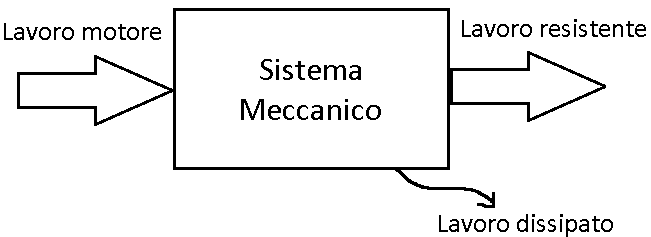
\includegraphics[width = 0.95\textwidth]{chapter05/Immagine85}
		\end{minipage}
		\hfill
		\begin{minipage}{0.5\textwidth}
			Il blocco \textbf{Sistema meccanico} rappresenta dunque l'insieme delle entità che interagiscono tra loro semplificando notevolmente il problema dinamico.
			
			Considerando un sistema meccanico generico l'equazione di bilancio dell'energia nell'intervallo \emph{dt} è data da:
			\[dL_e + dL_i = dE_C\]
		\end{minipage}
	\vspace{1mm}
	
	dove:
	\begin{itemize}
	\item $dL_e$ \hspace{2mm} Lavoro delle forze esterne applicate al sistema (\emph{motrice, resitenti, dissipative});
	\item $dL_i$ \hspace{2mm} Lavoro delle forze interne applicate al sistema (\emph{motrice, resistenti, dissipative});
	\item $dE_c$ \hspace{2mm} La variazione infinitesima di energia cinetica del sistema.
	\end{itemize}
	
	L'equazione può essere riordinata nella seguente forma, ricordando che il lavoro delle forze motrici, siano esse esterne o interne, \textbf{è sempre positivo} perché produce il moto mentre quello delle forze resistenti e dissipative, siano esse esterne o interne al sistema, \textbf{è sempre negativo} perché si oppone al moto:
	\[
	\underbrace{dL_M}_{\text{Forze motrici (>0)}} + \underbrace{dL_R}_{\text{Forze resistenti (<0)}} + \underbrace{dL_P}_{\text{Forze dissipate (<0)}} = dE_C
	\]
	
	Se rapportiamo gli scambi energetici al tempo \emph{dt}, nel quale hanno luogo, l'equazione può essere scritta in termini di potenza ($P = dL/dt$). Si ottiene in questo modo l'equazioni di bilancio della potenza, che lega le potenze delle forze applicate al sistema alla derivata temporale dell'energia cinetica:
	\[P_M + P_r + P_P = \td{E_c}{t}\]
	
	Qualora le forze interne ed esterne fossero di tipo conservativo il loro lavoro può essere espresso dall'energia potenziale $dL_e + dL_i = -dE_P$.
	L'integrazione dell'equazione dell'energia, espressa nella nuova forma, $-dE_P = dE_C$ fornisce l'integrale primo dell'energia:
	\[ E_C + E_P = cost.\]
	
	il quale mostra che la somma dell'energia potenziale e dell'energia cinetica è una costante e si verifica, in particolare, quando non v'è presenza di forze dissipative.
	
	\subsection{Esempi}
	\begin{enumerate}
	\item {\scshape{\bfseries Oscillatore armonico}}
	
	
	\begin{minipage}{.7\textwidth}
Consideriamo una massa sospesa elasticamente mediante una molla di rigidezza k.

 Poiché la forza elastica della molla è una forza conservativa, essa sarà in equilibrio con l'energia cinetica data dalla massa.
 
 Andando ad osservare gli andamenti temporali di velocità e posizione della massa rispetto alla sua posizione iniziale si possono trarre alcune conclusioni sulla configurazione di equilibrio del sistema in esame:
	\end{minipage}
	\hfill
	\begin{minipage}{.25\textwidth}
		\centering
		\includegraphics[width=.95\textwidth]{chapter05/Immagine86}
	\end{minipage}
	
	
	Procediamo dunque ad eseguire il bilancio di energia tra istanti diversi si tempo (t1 e t2).
	
	In t1: $X = 0$ e $\dot{X} = MAX$
	
	 lo spostamento è nullo e la molla è completamente rilassata.
	 
	 In t2: $X = MAX$ e $\dot{X} = 0$
	 
	  (configurazione di equilibrio tra forza peso e forza elastica della molla)	
	
	Il sistema meccanico proposto può dunque immagazzinare energia tramite due forme:
	\begin{gather*}
	 E_{pot} = \cfrac{1}{2}\,k\,x^2\qquad;\qquad E_C = \cfrac{1}{2}\,m\,\dot{x}^2
	\end{gather*}
	
	A t = $t_1$ \[E_{pot}+E_c = \cancel{\cfrac{1}{2}\,k\,x^2} + E_c = E_{c1} \]
	
	A t = $t_2$ \[E_{pot}+E_c = E_{pot} + \cancel{ \cfrac{1}{2}\,m\,\dot{x}^2} = E_{pot2}\]
	
	Poiché la legge del moto è del tipo armonico:
	
	 sia $x(t) = x_0\,\sin{(\omega\,t)}$ e il relativo andamento della velocità $\dot{x}(t) = \omega\,x_0\,\cos{(\omega\,t)}$
	
	Dal bilancio di energia tra i due istanti considerati si ottiene;
	\begin{gather*}
	E_{c1} = E_{pot2}\\
	\cancel{\cfrac{1}{2}}\,m\,(\omega^2\,\cancel{x_0^2}\,\cos^2{(\omega\,t)}) = \cancel{\cfrac{1}{2}}\,k\,\cancel{x_0^2}\,\sin^2{(\omega\,t)}\\
	m\,\omega^2\,\cos^2{(\omega\,t)}|_{t = 0}  = k\,\sin^2{\omega\,t}|_{t = \frac{2\,\pi}{\omega}\cdot\frac{1}{4}=\frac{\pi}{2\,\omega}} \\
	m\,\omega^2 = k\,\sin^2{(\cancel{\omega}\,\cfrac{\pi}{2\,\cancel{\omega}})}\\
	m\,\omega^2 = k\\
	\omega= \pm\,\sqrt{\cfrac{k}{m}}
	\end{gather*}

	\item {\scshape{\bfseries Carro contro un respingente}}

Si consideri il carrello rappresentato in figura inizialmento fermo ad una altezza \emph{h}.

	\begin{minipage}{.5\textwidth}
	
	 Nell'ipotesi di attrito nullo si voglia calcolare la velocità di arrivo, nella posizione 2 (un delta prima che il respingente sia compresso), e lo schiacciamento della molla tra le posizioni 2 e 3.
	 
	 Si può pervenire molto facilmente ad una soluzione considerando che la forza gravitazionale e la forza elastica del respingente sono di natura conservativa, per cui vale l'equazione:
	 \[E_{pot} + E_c = cost. = E_{tot}\]
	\end{minipage}
	\hfill
	\begin{minipage}{.5\textwidth}
	\centering
	\includegraphics[width=.9\textwidth]{chapter05/Immagine87}
	\end{minipage}

	L'istante/posizione 1 del carrello ha una $E_{tot} = E_{pot1}+ \cancel{E_c1} = mgh$
	
	L'istante/posizione 2 del carrello ha una $E_{tot} = \cancel{E_{pot2}} + E_{c2} = \cfrac{1}{2}\,m\,v^2$
	
	Da tali considerazioni si può ricavare la velocità del carrello, che risulta pari a:
	\begin{gather*}
	\cancel{m}gh = \cfrac{1}{2}\,\cancel{m}\,v^2\qquad\iff\qquad v = \sqrt{2gh}
	\end{gather*}
	
	L'istante/posizione 3 del carrello ha una $E_{tot} = E_{pot3} + \cancel{E_{c3}} = \cfrac{1}{2}\,k\,x_0^2$
	
	Dal bilancio energetico tra l'istante 2 e 3 si ottiene:
	
	\begin{gather*}
	\cancel{\cfrac{1}{2}}\,k\,x_0^2 = \cancel{\cfrac{1}{2}}\,m\,v^2\qquad\iff\qquad x_0 = \sqrt{\cfrac{m}{k}\,v^2} = v\,\sqrt{\cfrac{m}{k}} = \cfrac{v}{\omega}
	\end{gather*}
	
	Siamo pervenuti ad un'espressione della pulsazione naturale dell'oscillatore $\omega = \sqrt{\cfrac{k}{m}}$, grazie alla quale è possibile calcolare la forza massima che l'oscillatore/respingente deve sopportare:
	\[
	F_0 = k\,x_0 = \cfrac{kv}{\omega}
	\]

\newpage
	\item {\scshape{\bfseries Innesto di due volani}}
	
	\begin{minipage}{.5\textwidth}
	Due volani i cui momenti di inerzia sono rispettivamente $I_1$ e $I_2$ vengono collegati con un innesto a frizione.
	
	Calcolare la velocità di rotazione finale comune ai due volani e la dissipazione di energia prodotta dall'attrito.
	
	Il momento della quantità di moto di un sistema particellare è:
	\[\mathbf{K_0} = \sum_i{m_i}\cdot \mathbf{OP_i}\wedge\mathbf{v_i}\]
	\end{minipage}
	\hfill
	\begin{minipage}{.5\textwidth}
	\centering
	\includegraphics[width=.9\textwidth]{chapter05/Immagine88}
	\end{minipage}
	
		Il momento delle forze esterne rispetto ad un polo O o rispetto al baricentro del sistema, è invece:
	\[\sum{\mathbf{M_0}} = \td{\mathbf{K_0}}{t}\]
	
	All'innesto dei due dischi/volani la $\td{\mathbf{K_0}}{t} = 0$, in altri termini:
	\[\mathbf{K_0} = \mathbf{K_1}+\mathbf{K_2} = \mathbf{K_{tot}}\]
	dove: $\mathbf{K_1}$ e $\mathbf{K_2}$ sono rispettivamente i momenti della quantità di moto dei 2 volani.
	
	Tale relazione vale anche se l'energia non si conserva.
	
	Noto dunque che:
	\begin{gather*}
	K_{tot\,i} = I_1 \cdot \omega_1\qquad;\qquad K_{tot\,f} = (I_1 + I_2)\,\omega_f
	\end{gather*}
	
	Dal momento che il sistema è composto esclusivamente dai due volani e che non sono applicati al sistema momenti esterni:
	\begin{gather*}
		K_{tot\,i} = K_{tot_f}\\
		I_1\omega_1 = (I_1 + I_2)\,\omega_f\\
		\omega_f = \cfrac{I_1}{(I_1 + I_2)}\,\omega_1 
	\end{gather*}
	
	La variazione dell'energia cinetica è uguale al lavoro dissipato per attrito e trasformato in calore:
	\[ \int_i^f dL_i = \int_i^f dE_c = E_{cf} - E_{ci} = \cfrac{1}{2}\,(I_1 + I_2)\,\omega^2 - \cfrac{1}{2}I_1\omega_1^2 = -\cfrac{1}{2} \cfrac{I_1I_2}{I_1 + I_2} \omega_1^2\]
	
	Da osservare che il lavoro risulta negativo in quanto lavoro dissipato.
	\end{enumerate}
	
	\section{Equazione del moto con l'approccio energetico}
	
		Alla base di questo aproccio vi è l'equazione di bilancio della potenza:
		\[
			P = P_M + P_R + P_P = \td{E_C}{t}
		\]
		
		la potenza delle forze motrici è positiva mentre la potenza delle forze resistenti è negativa come la potenza persa dovuta alle forze di attrito. Alcune delle forze motrici e resistenti possono essere di natura conservativa, distinguiamo il contributo da quello delle forze non conservative:
		
		\[\underbrace{P_{con}}_{\text{per loro natura ammettono un potenziale}} + P_{N.\,con} = \td{E_c}{t}\]
		
		Il lavoro delle forze conservative può essere espresso in funzione delle variazioni di energia potenziale:
		
		\[dL_{con} = -dE_P\]		
		
		L'equazione della potenza può quindi essere scritta nella forma:
		
		\[P_{N.\,con} = \td{E_c}{t} + \td{E_p}{t}\]
		
		Nelle macchine ad alta velocità il termine preponderante al secondo membro è rappresentato dal tasso di variazione dell'energia cinetica, mentre nelle macchine lente e pesanti il termine preponderante può essere rappresentato dalla variazione dell'energia potenziale dovuta agli spostamenti verticali dei suoi membri.
		
		Oltre all' energia potenziale elastica immagazzinata nelle molle o in altri organi elastici può essere importante anche l'energia dissipata. La dissipazione ha luogo nei cuscinetti e nelle parti della macchina, dove le parti slittano o rotolano l'una rispetto all'altra, e negli smorzatori; i meccanismi di dissipazione sono l'attrito viscoso, l'attrito radente, l'attrito volvente. La dissipazione di energia ha come effetto il riscaldamento delle parti a contatto cui segue un flusso di calore dalla macchina all'ambiente circostante. L'energia è persa nel senso che si sottrae al possibile lavoro utile prodotto dalla macchina.
		
		Consideriamo una macchina piana ad 1 G.d.L. formata da corpi rigidi (\emph{eventuali molle hanno massa trascurabile}), ad esempio come quella rappresentata di seguito:
		
		\begin{minipage}{.5\textwidth}
		\centering
		\includegraphics[width=.95\textwidth]{chapter05/Immagine89}
		\end{minipage}
		\hfill
		\begin{minipage}{.5\textwidth}
		Determiniamo le caratteristiche della macchina, dinamicamente equivalente alla prima, costituita da una sola inerzia rotante, detta inerzia ridotta del sistema, sulla quale agisce una sola coppia, detto momento ridotto. \newline
		
		Da osservare che nel caso di movente traslante il meccanismo equivalente è costituito da una massa ridotta traslante sulla quale agisce una sola forza ridotta nella direzione del moto.
		\end{minipage}
	
	\begin{minipage}{.7\textwidth}
	Al fine di ricavare il sistema dinamicamente equivalente a quello proposto, è necessario conoscere le masse, i centri di massa, i momenti e i momenti d'inerzia di ogni singolo corpo.
	
	Nel caso di azioni di rotazione come coppie e momenti d'inerzia è preferibile definire per analogia una coordinata rotante.
	
	Il meccanismo equivalente così composto vogliamo che risponda allo stesso modo del meccanismo reale.
	\end{minipage}
	\hfill
	\begin{minipage}{.25\textwidth}
	\centering
	\includegraphics[width=.9\textwidth]{chapter05/Immagine90}
	\end{minipage}
	\vspace{1mm}
	
	Ciò è possibile imponendo l'uguaglianza delle due energie cinetiche dei membri 1 e 2 per trovare l'inerzia equivalente.
	
	\begin{align*}
	E_{c\,eq} &= \cfrac{1}{2} I^{*} \dot{q}^2\\
	&= E_{c\,G2} + E_{c\,rot} \\
	&= \sum_{i=1}^n (\cfrac{1}{2}\,m_i\,\dot{x_i}^2 + \cfrac{1}{2}\,m_i\,\dot{y_i}^2 + \cfrac{1}{2}\,I_i\,\dot{\theta_i}^2)
	\end{align*}
	
	Dove:
	\begin{itemize}
	\item i termini $\cfrac{1}{2} m_i \dot{x_i}^2$ e $\cfrac{1}{2} m_i \dot{y_i}^2$ rappresentano l'energia cinetica associata all'i-esimo centro di massa
	\item il termine $\cfrac{1}{2} I_i\dot{\theta_i}^2$ rappresenta il momento d'inerzia rispetto all'i-esimo centro di massa. 
	\end{itemize}
	
	Noto che il sistema sotto esame ha 1 G.d.L. tutte le velocità degli i-esimi centri di massa possono essere espresse come (derivanti dall'analisi cinematica del sistema):
	\begin{gather*}
	\dot{x_i} = \tau_{xi}\,\dot{q}	\qquad;\qquad	\dot{y_i} = \tau_{yi}\,\dot{q} \qquad;\qquad \dot{\theta_i} = \tau_{\theta i}\,\dot{q}
	\end{gather*}
	
	L'equazione dunque diviene:
	
	\begin{align*}
	\cancel{\cfrac{1}{2}}\,I^{*}\,\cancel{\dot{q}^2} &= \sum_{i=1}^n (\cancel{\cfrac{1}{2}}\,m_i\,\tau_{xi}^2\,\cancel{\dot{q}^2}+\cancel{\cfrac{1}{2}}m_i\,\tau_{yi}^2\,\cancel{\dot{q}^2} + \cancel{\cfrac{1}{2}}I_i\,\tau_{\theta i}^2 \cancel{\dot{q}^2})
	\end{align*}
	
	\begin{empheq}[box=%
	\fbox]{align*}
	I^{*} &= \sum_{i=1}^n(m_i\,\tau_{xi}^2 + m_i\,\tau_{yi}^2 + I_i\,\tau_{\theta i}^2) 
	\end{empheq}
	
	Il momento d'inerzia così ottenuto è detto \textbf{momento d'inerzia ridotto} e poiché contiene nella sua espressione i rapporti di velocità, i quali dipendono dalla configurazione, è anch'esso dipendente dal movente ``q'' scelto (I* = I*(q)).
	
	Le azioni della coppia Q* deve essere equivalente all'effetto delle azioni sul meccanismo reale.
	
	La potenza delle azioni coppie-forze deve essere uguale alla somma delle potenze delle azioni che agiscono sul meccanismo reale:
	\[
	P_{eq} = Q^*\,\dot{q} = \underbrace{\sum_{i=1}^{r} (F_{xi}\cdot\dot{x_i}\,+ F_{yi}\cdot\dot{y_i})}_{\text{Potenza delle forze applicate}} + \underbrace{\sum_{i=1}^{s}(M_i\,\dot{\theta_i})}_{\text{Potenza dei momenti applicati}}
		\]
	
	Si tenga presente che le potenze delle forze applicate sono moltiplicate per la velocità delle coordinate $(x_i,y_i)$ che non sono necessariamente i centri di massa, bensì i punti a cui è applicata la forza.
	
	\[
	Q^*\,\cancel{\dot{q}} = \sum_{i=1}^r (F_{xi}\tau_{xi}\cancel{\dot{q}} + F_{yi}\,\tau_{yi}\cancel{\dot{q}}) + \sum_{i=1}^s(M_i \tau_{\theta i }\cancel{\dot{q}})
	\]
	\begin{empheq}[box=%
	\fbox]{equation*}
		Q^* = \sum_{i=1}^r(F_{xi}\tau_{xi} + F_{yi}\tau_{yi}) + \sum_{i=1}^s (M_i\,\tau_{\theta i}) = Q^*(q,t)
	\end{empheq}
	
	La relazione così ottenuta esprime il momento ridotto del sistema dinamicamente equivalente con una relazione di dipendenza dalla configurazione (derivante dalla presenza dei rapporti di velocità) e temporale (F(t), M(t)).
	
	
	Una volta ricavata l'espressione del momento ridotto e del momento d'inerzia ridotto è possibile scrivere l'equazione della potenza:
	
	\begin{align*}
	Q^*\,\dot{q} &= \td{}{t}(\cfrac{1}{2}\,I^* \,\dot{q}^2)\\
	&= \cfrac{1}{2} \td{I^*}{t}\,\dot{q}^2\,+\,\cfrac{1}{2}\,I^*(\td{\dot{q}^2}{t})\\
	&= \cfrac{1}{2}\,\td{I^*}{q}\,\td{q}{t}\,\dot{q}^2 + \cfrac{1}{2}\,I^* (\td{\dot{q^2}}{\dot{q}}\,\td{\dot{q}}{t})\\
	Q^*\cancel{\dot{q}} &= \cfrac{1}{2}\,\td{I^*}{q}\,\dot{q}^{\cancelto{2}3} + \cfrac{1}{\cancel{2}}\,I^*\,\cancel{2}\,\cancel{\dot{q}}\ddot{q}
	\end{align*}
	
	\begin{empheq}[box=%
	\fbox]{align*}
		Q^*= \cfrac{1}{2}\,\td{I^*}{q}\dot{q}^2 + I^*\,\ddot{q}
	\end{empheq}
	
	Questa equazione, se sono assegnate le forze e le coppie motrici e resistenti e le condizioni iniziali, consente di calcolare l'andamento temporale di \emph{q}
.

Anche il termine \emph{dI* / dq} dipende solo dalla posizione. Infatti si può scrivere:

\begin{align*}
\cfrac{1}{2} \td{I^*}{q} &= \cfrac{1}{\cancel{2}} \sum_{i=1}^n (\cancel{2}\, m_i\,\tau_{xi}\td{\tau_{xi}}{q} + \cancel{2}\, m_i\,\tau_{yi}\td{\tau_{yi}}{q} + \cancel{2}\, I_i\,\tau_{\theta i}\td{\tau_{\theta i}}{q})\\
&= \sum_{i=1}^n (m_i\,\tau_{xi}\,\td{\tau_{xi}}{q} + m_i\,\tau_{yi}\,\td{\tau_{yi}}{q} + I_i\,\tau_{\theta i}\,\td{\tau_{\theta i}}{q})
\end{align*}
	
	I derivati dei rapporti di velocità risultano:
	\begin{align*}
		\td{\tau_{xi}}{q} = \td{\cfrac{\dot{x_i}}{\dot{q}}}{q} &= \cfrac{\ddot{x_i}\,\cancel{\cfrac{\dot{q}}{\dot{q}}}  - \dot{x_i}\,\cfrac{\ddot{q}}{\dot{q}}}{\dot{q}^2}\\
&= \cfrac{\ddot{x_i} - \dot{x_i}\,\cfrac{\ddot{q}}{\dot{q}}}{\dot{q}^2}\\
&= \cfrac{\ddot{x_i} - \tau_{xi}\ddot{q}}{\dot{q}^2}
	\end{align*}
	
	\subsection{Forze e momenti funzione della posizione}
	
	Se le forze applicate al sistema sono funzioni esplicite delle sole posizioni (e \emph{non del tempo o delle velocità}), l'equazione dell'energia può essere risolta tramite due integrazioni successive.
	
	Sia Q* = Q*(q) e I* = I*(q), allora:
	
	\begin{align*}
	Q^*\,\dot{q} &= \td{}{t}(\cfrac{1}{2}\,I^*\,\dot{q}^2) = \td{}{q}(\cfrac{1}{2}\,I^*\,\dot{q}^2) \td{q}{t}\\
	&= \td{}{q}(\cfrac{1}{2}\,I^*\,\dot{q}^2)\,\dot{q}\\
	Q^*\,\cancel{\dot{q}}\, dq &= d (\cfrac{1}{2}\,I^*\,\dot{q}^2)\,\cancel{\dot{q}}
	\end{align*}
	
	Come si può evincere dalla relazione appena ottenuta il \emph{rhs} in quanto differenziale esatto risulta essere una primitiva del \emph{lhs}, perciò alla sua integrazione dipenderà esclusivamente dagli estremi di integrazione.
	
	Definito \textbf{stato 1} lo stato iniziale del sistema indicato con la sintassi ($q_1, \,\dot{q_1}$), si vuole conoscere l'evoluzione del sistema nello stato ($q_2,\dot{q_2}$):
	
	\begin{align*}
		\int_{q_1}^{q_2} Q^*(q)\,dq &= \int_{q_1}^{q_2} d (\cfrac{1}{2}\,I^*(q)\,\dot{q}^2) = 	\Bigl(\cfrac{1}{2}\,I^*(q)\,\dot{q}^2\Bigr)\Bigr|_{q_1}^{q_2}\\
		&= \cfrac{1}{2}\,I^*(q_2)\,\dot{q_2}^2 - \cfrac{1}{2}\,I^*(q_1)\,\dot{q_1}^2 
	\end{align*}
	
	Noto dunque lo stato iniziale e la funzione Q*(q), si può determinare la rimanente incognita:
	\[
	\dot{q_2} = \cfrac{\sqrt{(\int_{q_1}^{q_2} Q^*(q)\,dq) + \cfrac{1}{2}\,I^*(q_1)\,\dot{q_1}^2}}{\cfrac{1}{2}\,I^*(q_2)}
	\]
	
	\subsection{Forze non conservative}
	
	È noto dai paragrafi precedenti che l'equazione della potenza nel caso di compresenza di forze conservative e non è pari a :
	
	\begin{align*}
	P_{N.\,con.} &= \td{E_c}{t} + \td{E_{pot.}}{t}\\
	Q^*\,\dot{q} &= \td{}{t}(\cfrac{1}{2}\,I^*\,\dot{q}^2)\,+\,\td{E_{pot}}{t}\\
	Q^*\,\dot{q} &= \cfrac{1}{2}\td{I^*}{t}\dot{q}^2 \,+\,I^*\dot{q}\ddot{q}\,+\,\td{E_{pot}}{t}\\
	Q^*\,\dot{q} - \td{E_{pot}}{t} &= \cfrac{1}{2}\td{I^*}{t}\dot{q}^2 \,+\,I^*\dot{q}\ddot{q}\\
	(Q^*\,-\,\cfrac{1}{\dot{q}}\,\td{E_{pot}}{t})\,\dot{q} &= \cfrac{1}{2}\td{I^*}{t}\dot{q}^2 \,+\,I^*\dot{q}\ddot{q}
	\end{align*}
	
	\begin{empheq}[box=%
	\fbox]{align*}
	(Q^* + Q^*_{pot})\,\dot{q} =  \cfrac{1}{2}\td{I^*}{t}\dot{q}^2 \,+\,I^*\dot{q}\ddot{q}
	\end{empheq}
	
	
	Finora non abbiamo fatto alcuna distinzione tra le forze applicate (\emph{forze conservative e non}) nel calcolo ella potenza. Vediamo ora di esplicitare la potenza nel caso di forze peso, di forze elastiche, di forze dissipative di tipo viscoso e di forze dissipative di tipo Coulombiano.
	
	\begin{enumerate}
	\item {\scshape{\bfseries Forza Peso}}
		Nel caso di forze peso l'energia potenziale dovuta all'elevazione del corpo rigido al di sopra di un certo livello di riferimento è:
		\[E_{pot} = mgh\]
		Il relativo contributo da sommare alla forza ridotta risulterà dunque essere:
		\[
		Q^*_{peso} = -\,\cfrac{1}{\dot{q}}\,(\td{E_{pot}}{t}) = -\,\cfrac{1}{\dot{q}}\,\td{(mgh)}{t} = -\,\cfrac{\dot{h}}{\dot{q}}\,mg = -\,mg\tau_h
		\]
		ed è funzione solo di q in quanto il rapporto di velocità $\tau_h$ è funzione di q.
	\item  {\scshape{\bfseries Forza Elastica}}
	L'energia potenziale di una molla lineare è data dall'espressione:
	\[
	E_{pot} = \cfrac{1}{2}\,k\,(s-s_0)^2
	\]
	dove \emph{k} è la costante elastica della molla, s è il vettore che congiunge gli estremi della molla e $s_0$ è lo stesso vettore prima della deformazione.
	
	La derivata risulta:
	\[
	\td{E_{pot}}{t} = k\,(s-s_0)\,\dot{s}
	\]
	e la forza ridotta:
	\[
	Q^*_{elastica} = -\,\cfrac{k(s-s_0)\dot{s}}{\dot{q}} =-\, k(s-s_0)\tau_s
	\]
	Essa dipende da \emph{s} che è funzione di \emph{q} e dal rapporto di velocità che è pure funzione di \emph{q}.
	
	\item  {\scshape{\bfseries Forza Viscose}}
	
	Se le forze di attrito sono schematizzabili con un modello di tipo viscoso, la forza necessaria per muovere relativamente gli elementi di uno smorzatore viscoso è data da:
	\[
	F_{viscoso} = - c\dot{s}
	\]
	dove \emph{c} è il coefficiente di smorzamento viscoso e $\dot{s}$ è il modulo della velocità relativa tra i due elementi dello smorzatore. La potenza dissipata da uno smorzatore è data da:
	\[
	P = -\,c\,\dot{s}\,\dot{s}
	\]
	La forza ridotta risulta:
	\[
	Q^*_{viscoso} = -\,\cfrac{P}{\dot{q}} = -\,\cfrac{c\,\dot{s}\,\dot{s}}{\dot{q}} = -\,c\,\dot{s}\cfrac{\dot{q}}{\dot{q}}\,\tau_s = -\,c\,\dot{q}\,\tau_s^2
	\]
	ed anche in questo caso è funzione della coordinata generalizzata e delle sue derivate.
	
	\item  {\scshape{\bfseries Attrito Coulombiano}}
	Supponiamo ora che la natura della macchina sia tale per cui non possono essere trascurate le forze di attrito di tipo Coulombiano. In generale una forza di attrito Coulombiano può scriversi nella forma:
	\[
	F_{Coulomb} = - \mu_d\,\norma{N}\,\emph{vers}(\und{\nu})
	\]
	Dove $-vers(\und{\nu})$ è un vettore che si oppone al moto, ovvero si oppone al vettore velocità
	
	La corrisponente potenza dissipata vale:
	\[
	P_{Coulomb} = -\,\mu_d\,\norma{N}\,vers(\und{\nu})\,\nu = -\,\mu_d\,\norma{N}\,vers(\und{\nu})\,\tau_{\nu}\,\dot{q}
	\]
	Ed è funzione di q e della componente della forza reattiva $\norma{N}$.
	
Pertanto, a differenza di tutti gli altri casi considerati, in questo termine compare una forza reattiva. Perciò l'equazione del moto, in presenza di attrito Coulombiano conterrebbe oltre all'incognita \emph{q} anche una seconda incognita, perciò da sola non è sufficiente a risolvere il problema.

Per risolvere il problema bisogna affiancare all'equazione del moto l'equazione di equilibrio dei vari membri; in questo caso allora può essere più vantaggioso effettuare l'analisi dinamica direttamente con l'approccio Newtoniano.
	
	\end{enumerate}
	
	\section{Analisi dinamica del manovellismo di spinta}
	\begin{minipage}{.5\textwidth}
	Consideriamo il meccanismo di spinta centrato e supponiamo che la manovella motrice sia bilanciata e che la biella abbia massa trascurabile. Manovella motrice bilanciata significa che il baricentro della manovella è coincidente con il perno di banco A. Vogliamo scrivere l'equazione del moto.
	
	Determiniamo l'inerzia ridotta, considerando trascurabile l'inerzia della biella:
	\[
	I^* =\sum (m_i\,\tau_i^2 + I_i\,\tau_{\theta i}^2) = I_A\,\tau_{\theta1}^2 + m_c\,\tau_{xi}^2
	\]
	\end{minipage}
	\hfill
	\begin{minipage}{.5\textwidth}
	\centering
	\includegraphics[width=.95\textwidth]{chapter05/Immagine91}
	\end{minipage}
	Noto che $\tau_{\theta1 = q} = \cfrac{\dot{q}}{\dot{q}} = 1$

	Il momento d'inerzia ridotto sarà pari a: $I^* = I_A + m_c\,\tau_{xi}^2$
	
	Calcoliamo a questo punto Il momento ridotto ponendo in uguaglianza le due espressioni che abbiamo ricavato:
	\begin{gather*}
		Q^* = \cfrac{1}{2}\,\td{I^*}{q}\,\dot{q}^2 + I^*\,\ddot{q}\qquad;\qquad 	Q^* = \sum_{i=1}^r(F_{xi}\tau_{xi} + F_{yi}\tau_{yi}) + \sum_{i=1}^s (M_i\,\tau_{\theta i})
	\end{gather*}
	
	
	La derivata dell'inerzia ridotta rispetto alla coordinata libera risulta:
	\[
	\cfrac{1}{2}\td{I^*}{q} = m_C\,\tau_{xi}\,\td{\tau_{xi}}{q}
	\]
	
	La coppia ridotta dipende dal momento motore applicato alla manovella e dalla forza resistente applicata al pistone:
	\[
	Q^* = M(t)\,\tau_{\theta1}\,+\,F(t)\,\tau_{xi} = M(t) + F(t)\,\tau_{xi}
	\]
	È necessario conoscere il rapporto di velocità relativo alla traslazione del pattino (\emph{punto C}) e il suo derivato.
	
	Nell'ipotesi che la biella abbia lunghezza molto maggiore della lunghezza della manovella (\emph{c/r} > 4), si sono determinate delle espressioni analitiche approssimate sia per il rapporto di velocità che per la sua derivata.
	\begin{gather*}
	\tau_{xi}\approx -\,r\,(\sin{q} + \cfrac{r}{c}\,\cfrac{\sin{(2q)}}{2})\qquad;\qquad \td{\tau_{xi}}{q} = -\,r\,(\cos{q}+\cfrac{r}{c}\,\cos{(2q)})
	\end{gather*}
	L'equazione del moto:
	\[
	I^*(q)\,\ddot{q} + \cfrac{1}{2}\td{I^*(q)}{q}\,\dot{q}^2= Q^*	
	\]
	si può quindi esplicitare in funzione della sola coordinata libera sostituendo $I^*(q), \td{I^*(q)}{q},Q^*$ con le espressioni trovate.
	
	\section{Rendimento di un sistema meccanico}
	
	\begin{minipage}{.3\textwidth}
	\centering
	\includegraphics[width=.95\textwidth]{chapter05/Immagine92}
	\end{minipage}
	\hfill
	\begin{minipage}{.7\textwidth}
	Scatola nella quale entra un lavoro motore, esce un lavoro resistente e dissipato.
	
	 Inoltre il sistema può accumulare energia sotto forma di energia cinetica.

	Consideriamo di nuovo l'equazione dell'energia applicata ad una macchina nell'intervallo $\Delta t$:
	\end{minipage}
	
	\[L_M + L_R + L_D = \Delta E_c\]	
	dove
	\begin{itemize}
	\item $L_M$ è il lavoro positivo compiuto dalle forze motrici nell'intervallo $\Delta t$;
	\item $L_R$ è il lavoro compiuto dalle forze resistenti e quindi negativo;
	\item $L_D$ è il lavoro, di valore negativo, compiuto dalle forze dissipative, sempre nell'intervallo $\Delta t$.
	\end{itemize}
	
	Se la macchina funziona \emph{in regime assoluto} la velocità di tutti i membri è costante nel tempo per cui $\Delta E_c = 0$ per ogni valore di $\Delta t$ e l'equazione si riduce a:
	\[L_M + L_R + L_P = 0\]
	Tale bilancio di energia vale quando il sistema ha finito di accumulare energia cinetica e la mantiene costante nel tempo.
	
	Essendo nulla anche la derivata dell'energia cinetica vale anche la relazione in termini di potenza:
	\[
	P_M + P_R + P_D = 0
	\]
	Se la macchina funziona \emph{in regime periodico} la velocità di tutti i membri si ripetono ad intervalli pari al periodo.
	
	$E_c(t) = E_c(t+T_F)$ dove $T_F$ è il periodo.
	
	Il bilancio energetico sotto tali ipotesi è sempre pari a:
	\[L_M + L_R + L_P = 0\]
	sia che il moto sia permanente, sia che si compia il bilancio tra due istanti in fase in un regime periodico.
	
	Tuttavia in questo caso non vale l'equazione in termini di potenza in quanto in generale $\td{E_c}{t}\ne0$ e quindi:
	\[P_M + P_R + P_D \ne 0\]
	Con riferimento ad una macchina funzionante in regime assoluto o in regime periodico, considerando in questo caso intervalli di tempo multipli del periodo, si definisce \textbf{rendimento} il rapporto tra il modulo del lavoro resistente utile e il lavoro motore:
	\[
	\eta = \cfrac{\norma{L_R}}{L_M} = \cfrac{L_M - \norma{L_D}}{L_M} = 1 - \cfrac{\norma{L_D}}{L_M} = \cfrac{\norma{L_R}}{\norma{L_R}+\norma{L_D}}  \qquad(<1)
	\]
	Il rendimento è un numero adimensionale, ed è sempre minore di 1 per la presenza nella realtà di forze resistenti passive. Se la macchina funziona in regime assoluto il rendimento può essere espresso anche in termini di potenza, nella forma:
	\[
	\eta = \cfrac{\norma{P_R}}{P_M} = \cfrac{P_M - \norma{P_D}}{P_M} = 1 - \cfrac{\norma{P_D}}{P_M} = \cfrac{\norma{P_R}}{\norma{P_R} + \norma{P_D}}
	\]
	Al rendimento può essere data anche una espressione diversa. Se supponiamo che la macchina funzioni in condizioni ideali, cioè in assenza di forze resistenti passive, e sia sottoposta alla stessa forza resistente nel caso reale, in condizioni di regime assoluto o periodico avremo:
	\[
	L_{Mi} + L_{R} = 0\qquad\Leftarrow\qquad L_{Mi} = \norma{L_R}
	\]
	dove con $L_{Mi}$ si è indicato il lavoro motore richiesto in questa situazione puramente ideale. Perciò, tenendo conto della definizione di rendimento si ottiene:
	\[
	\eta = \cfrac{\norma{L_R}}{L_M} = \cfrac{L_{Mi}}{L_M}
	\]
	Ossia il rendimento è anche dato dal rapporto tra il lavoro motore in condizioni ideali e il lavoro motore in condizioni reali, necessari per contrastare lo stesso lavoro resistente. Se la macchina funziona in regime assoluto tale relazione può essere espressa anche in termini di potenza.
	
	Queste relazioni mostrano che a causa delle resistenza passive il lavoro motore reale è sempre maggiore di quello ideale.
	
	È possibile determinare il rendimento complessivo di una macchina o di un gruppo di macchine fra loro collegate:
	
	\subsection{Rendimento di macchine disposte in serie}
	
	Nel collegamento in serie il lavoro resistente di una macchina eguaglia quello motore della macchina che la segue e con la quale scambia energia.
	\begin{center}
	\includegraphics[width=.8\textwidth]{chapter05/Immagine93}
	\end{center}
	
	Applicando la definizione, poiché $\norma{L_{R\,i}} = L_{M\,i+1}$ si ottiene:
	
	\begin{align*}
	\eta_s &= \cfrac{\norma{L_R}}{L_M} = \cfrac{L_{R\,n}}{L_{M\,n}}\cdot\cfrac{\norma{L_{R\,n-1}}}{L_{M\,n-1}}\dots\cfrac{\norma{L_{R\,2}}}{L_{M2}}\cdot\cfrac{\norma{L_{R\,1}}}{L_{M\,1}}\\
	&= \eta_n\cdot\eta_{n-1}\dots\eta_2\cdot\eta_1
	\end{align*}
	
	Perciò il rendimento globale è il prodotto dei rendimenti delle singole macchine. Se una sola macchina ha un basso rendimento tutto il sistema ha un basso rendimento.
	\begin{center}
\line(1,0){250}
\end{center}

\section{Lezione 01-04 -- Daniele Boroluzzi}

Riprendiamo alcuni concetti che abbiamo già esposto nelle sottosezioni precedenti: in paricolare partiamo dal concetto di rendimento di un sistema meccanico. Come viene solitamente diagrammato, si rappresenta il sistema tramite uno schema a blocchi in cui sono presenti:
\begin{itemize}
\item Una freccia entrante a rappresentare il lavoro motore che entra nel sistema meccanico in esame
\item Una freccia uscente a rappresentare il lavoro resistente
\item Una freccia uscente a rappresentare il lavoro dissipato
\item In generale il nostro sistema può accumulare energia nella forma cinetica, per questo tale componente di energia viene rappresentata all'interno del blocco.
\end{itemize}

Quindi, è possibile scrivere un primo bilacio di energia:
\[L_m + L_r + L_p = \Delta E_C\]
E tale bilancio deve valere in genere in virtù del pricipio di conservazione dell'energia.

Supponiamo ora di avere un funzionamento a regime, ovvero un funzionamento in cui l'energia del sistema (in forma cinetica) non varia ($\Delta E_c = 0$), il bilancio di energia si può semplicemente riscrivere come:
\[L_m + L_r + L_p = 0\] 
Tale situazione si osserva quando il sistema ha terminato di accumulare energia cinetica e la mantiene costantenel tempo. Possiamo, inoltre, pensare che tale bilancio di energia possa essere espresso anche in termini di bilancio di potenze, per cui è possibile anche scrivere che la derivata dell'equazione precedente sia comunque uguale a zero e quindi:
\[P_m + P_r + P_p = 0\]
C'è da precisare che per definizione in questo sistema la potenza (o anche il lavoro motore) è positivo, in altri termini vi è energia che entra nel nostro sistema, e che il lavoro resistente è negativo, di conseguenza dove è presente l'utenza della macchina che preleva l'energia necessaria, e il lavoro dissipato negativo che chiude il bilancio a zero.

In realtà le equazioni che abbiamo scritto, sotto l'ipotesi di $\Delta E_c = 0$, può valere anche non necessariamente quando l'energia cinetica è costante, ma vale anche in regime periodico in cui l'energia cinetica presenta una certa ciclicità che si ripete nel tempo di periodo \textbf{T} e quindi in un periodo è possibile scrivere che l'energia cinetica raggiunge lo stesso valore all'inizio e alla fine del ciclo. In altri termini $E_c(t) = E_c(t+T)$.

Una volta definito in questo modo il sistema, come cioè un oggetto che riceve energia dal lato motore e la restituisce al lato resistente dissipandone una certa parte, è utile definire il \textbf{rendimento del sistema meccanico} come un rapporto ciò che si ottiene dal sistema ($L_r$) e ciò che gli viene fornito ($L_m$).
\[\eta = \cfrac{\norma{L_R}}{L_M} = \cfrac{L_M - \norma{L_P}}{L_M} = 1\,-\,\cfrac{\norma{L_P}}{L_M} = \cfrac{\norma{L_R}}{\norma{L_R}\,+\,\norma{L_P}}\,<\,1\]
Quanto formulato in termini di lavori può essere espresso in termini di potenze, quindi in termini di flusso di energia nell'unità di tempo
\[\eta = \cfrac{\norma{P_R}}{P_M} = \cfrac{P_M - \norma{P_P}}{P_M} = 1\,-\,\cfrac{\norma{P_P}}{P_M} = \cfrac{\norma{P_R}}{\norma{P_R}\,+\,\norma{P_P}}\,<\,1\]
\newline
Pensiamo adesso al medesimo sistema meccanico in condizioni ideali, ovvero nelle condizioni in cui la potenza dissipata che è presente nel nostro sistema sia nulla ($L_P = 0$, non sono presenti perdite). Supponiamo, inoltre, che si trovi in condizioni di funzionamento dettate dallo stesso lavoro resistente o potenza resistente, quindi l'utenza della nostra macchina riceve esattamente lo stesso lavoro/potenza di quella nelle condizioni non ideali e in tali condizioni di funzionamento ideali ci chiediamo: come può funzionare il nostro sistema?

Il bilancio dei lavori suggerisce che: in condizioni ideali di assenza di lavoro dissipato basterà un lavoro motore minore per far funzionare il sistema. In altri termini il lavoro motore in condizioni ideali ($L_{M,i}$) + il lavoro resistente ($L_R$) è pari a zero, in quanto non vi è nè accumulo di energia nel nostro sistema e non è presente energia dissipata.

L'equazione, in questo caso, diventa molto semplice e intuitiva perché ci dice che il lavoro motore in condizioni ideali è uguale in valore assoluto al lavoro resistente:
\[L_{M,i} = \norma{L_R}\]
Non essendoci alcun altra forma in cui questo lavoro motore viene accumulato o dissipato, va interamente all'utenza e di conseguenza vale l'uguaglianza in forma stretta.

Possiamo a questo puto calcolare il rendimento di questo caso di riferimento ideale come:
\[\eta = \cfrac{\norma{L_R}}{L_M} = \cfrac{L_{M,i}}{L_M} = \cfrac{P_{M,i}}{P_M}\]

Ci chiediamo a questo punto cosa succede al funzionamento di un sistema di macchine, quindi di un sistema di macchine connesse tra loro una volta noto il rendimento di ciascuna di esse.
\vspace{1mm}

\begin{minipage}{.5\textwidth}
Supponiamo quindi di avere \emph{n} macchine che sono disposte in serie, per cui il flusso di lavoro che esce dalla prima macchina è interamente indirizzato verso la seconda macchina e costituisce lavoro motore di quest'ultima e così via per le successive.
\end{minipage}
\hfill
\begin{minipage}{.5\textwidth}
\centering
\includegraphics[width=.95\textwidth]{chapter05/Immagine93}
\end{minipage}
\vspace{1mm}

Ci chiediamo anche in questo caso che rendimento possa avere la disposizione in serie di queste macchine. Compiamo dunque delle semplici considerazioni chiamando in causa le definizioni che abbiamo dato precedentemente.
\[\norma{L_{R,i}} = L_{M,(i+1)}\]
Attraverso la definzione dei rendimenti delle macchine che abbiamo dato precedentemente possiamo esprimere il rendimento complessivo del sistema di macchine come:
\[\eta_S = \cfrac{\norma{L_R}}{L_M} = \cfrac{\norma{L_{Rn}}}{L_{Mn}}\cdot\cfrac{\norma{L_{R\,n-1}}}{L_{M\,n-1}}\,\dots\,\cfrac{L_{R1}}{L_{M1}} = \eta_n\,\cdot\,\eta_{n-1}\,\dots\,\eta_1\]
Abbiamo cioé sfruttata l'identità tra il lavoro motore della macchina a monte e il lavoro resistente della macchina a valle per scrivere una serie di rapporti ed esprimere il rendimento complessivo come prodotto dei singoli rendimenti di ciascuna macchina.

La considerazione più importante da fare su tale espressione è che il rendimento della serie, essendo calcolabile come prodotto di rendimenti delle singole macchina, fa sì che sia influenzato allo stesso modo dai fattori della sua espressione in egual misura: basta che uno solo dei rendimenti sia molto basso per inficciare il rendimento di tutta la serie di macchine.

\subsection{Rendimento di macchine in parallelo}

\begin{minipage}{.5\textwidth}
Ci occupiamo ora della disposizione in parallelo delle macchine; supponiamo di avere tre macchine che sono attraversate da dei flussi di energia di cui è noto il singolo rendimento ($\eta_1, \eta_2$ e $\eta_3$), ognuna di queste riceve il lavoro motore che le compete ($L_{M1}, L_{M2}$ e $L_{M3}$), complessivamente questi lavori motori sono forniti al sistema di macchine e la loro somma è $L_M$.
\end{minipage}
\hfill
\begin{minipage}{.5\textwidth}
\centering
\includegraphics[width=.95\textwidth]{chapter05/Immagine150}
\end{minipage}
\vspace{1mm}

Ciascuna delle macchine in esame avrà il suo lavoro resistente ($L_{R1}, L_{R2}$ e $L_{R3}$), la cui somma restituisce il lavoro complessivamente fornito dal sistema di macchine che risulta essere $L_R$. Applichiamo la definizione di rendimento a questo sistema di macchine:
\[\eta = \cfrac{\norma{L_{R1}}\,+\,\norma{L_{R2}}\,+\,\dots\,+\,\norma{L_{R3}}}{L_M} = \cfrac{L_{M1}\,\eta_1\,+\,L_{M2}\,\eta_2\,+\,\dots\,+\,L_{Mn}\,\eta_n}{L_M}\]
Il rendimento dunque può essere interpretato come la media pesata dei rendimenti, i coefficienti di peso sono i lavori motore delle singole macchine. Il problema caratteristico della disposizione in serie viene mitigato in quanto anche se una macchina di quelle presenti nel sistema avesse un rendimento molto basso andrebbe a influenzare il rendimento complessivo del sistema in maniera inferiore nella misura in cui il lavoro che la attraversa è limitato, di conseguenza il fatto di pesare i rendimenti con il flusso effettivo di potenza rende questa espressione meno sensibile al rendimento di ciascuna macchina in quanto è pesato sul lavoro motore effettivo che la macchina riceve.

Possiamo ora focalizzarci sulla stessa definizione di rendimento per un parallelo di macchine prendendo in esame, anziché i lavori motore di ciascuna macchina, i lavori resistenti di ciascuna macchina: stiamo cioé cercando un'espressione del rendimento in cui i coefficienti dei rendimenti non siano più i lavori motore, ma quelli resistenti.

Per fare ciò sfruttiamo la definizione alternativa del rendimento:
\[\eta = \cfrac{\norma{L_R}}{L_{M1}\,+\,L_{M2}\,+\,\dots\,+\,L_{Mn}} = \cfrac{\norma{L_R}}{\cfrac{\norma{L_{R1}}}{\eta_1}\,+\,\cfrac{\norma{L_{R2}}}{\eta_2}\,+\,\dots\,+\,\cfrac{\norma{L_Rn}}{\eta_n}}\]
Questa espressione descrive ugualmente il rendimento del parallelo di macchine in funzione dei rendimenti di ciascuna macchina, ma in questo caso lo esprime in maniera pesata su i lavori resistenti. Tale espressione, matematicamente diversa da quella sviluppata con i lavori motore, prende il nome di \textbf{media armonica pesata}. 

È una media pesata sui lavori resistenti dei rendimenti delle varie macchine; anche in questo caso è evidente che il contributo di ciascuna macchina è pesato dal lavoro (resistente) che le compete, però il concetto che esprime è sempre lo stesso: una macchina che sia attraversata da un flusso di lavoro limitato all'utenza rende il termine i-esimo del lavoro resistente poco influente sulla somma presente al denominatore.

\subsection{Moto diretto e retrogrado}
Proviamo ora a ragionare su cosa succede invertendo il ruolo dell'organo motore della nostra macchina e dell'organo resistente. Eseguiamo questo esperimento ideale di invertire il ruolo di questi due membri della stessa macchina e proviamo a caratterizzare il fatto che tale macchina possa in qualche modo funzionare con un ruolo invertito tra movente e cedente una volta noto il rendimento,

\begin{center}
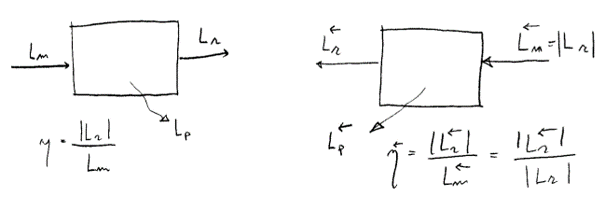
\includegraphics[width=.95\textwidth]{chapter05/Immagine151}
\end{center}

Partiamo dalla macchina generica il cui schema a blocchi è rappresentato sulla sinistra che riceve il lavoro $L_M$, fornisce il lavoro $L_R$ all'utenza e dissipa il lavoro $L_P$ a causa di fenomeni di attrito, etc...

Il rendimento, per definizione, è espresso come $\eta = \cfrac{\norma{L_R}}{L_M}$ per quanto riguarda la macchina in \textbf{moto diretto}.

Idealmente invertiamo il ruolo di movente e cedente e quindi immaginiamo che sia l'organo cedente a promuovere il moto della nostra macchina e all'organo movente vi sia l'utenza della macchina stessa, come rappresentato dallo schema a blocchi a destra. In esso i sensi delle frecce sono invertiti e il lavoro motore del \textbf{moto retrogrado} sia idealmente uguale al lavoro resistente che la macchina aveva in condizioni di moto diretto.

In altre parole il lavoro che la macchina prima forniva all'utenza diventa invece il lavoro che la macchina riceve per muoversi in senso opposto a quello che aveva inizialmente nel moto diretto.

In questo regime di funzionamento retrogrado la macchina avrà un qualche funzionamento per il quale ci sarà una certa dissipazione ($L_P$ retrogrado). Applichiamo ora la definizione di rendimento anche a questo caso:
\[\ret{\eta} = \cfrac{\norma{\ret{L_R}}}{\ret{L_M}} = \cfrac{\norma{\ret{L_R}}}{\norma{L_R}}\]
Calcoliamo alcune grandezze della macchina in moto diretto e retrogrado, in particolare la \textbf{perdita di rendimento}, che definiamo come il complemento a 1 del rendimento stesso:
\[1-\eta = 1\,-\,\cfrac{\norma{L_R}}{L_M} = \cfrac{\norma{L_P}}{L_M}\qquad;\qquad 1-\ret{\eta} = 1\,-\,\cfrac{\norma{\ret{L_R}}}{\ret{L_M}} = \cfrac{\norma{\ret{L_P}}}{\ret{L_M}}=\cfrac{\norma{\ret{L_P}}}{\norma{L_R}}\]
I lavori dissipati in moto diretto e retrogrado sono, in generale, diversi, però esprimiamo tramite in parametro K il loro rapporto:
\[K = \cfrac{\norma{\ret{L_P}}}{\norma{L_P}}\]
Proviamo sotto tale considerazioni a calcolare il rapporto tra le perdite di rendimento tra i due casi, ovvero studiamo qual è la prestazione della macchina in moto retrogrado rispetto alla prestazione in moto diretto, ricordando che la perdita di rendimento è un valore che, tanto più è piccolo, quanto meglio la macchina sta funzionando:
\[\cfrac{1-\ret{\eta}}{1-\eta} =  \cfrac{\norma{\ret{L_P}}}{\norma{L_R}}\,\cdot\,\cfrac{L_M}{\norma{L_P}} = \cfrac{K}{\eta}\]
Nell'equazione appena scritta possiamo pensare che l'incognita sia il rendimento del moto retrogrado:
\[\ret{\eta} = \cfrac{\eta\,(1+K) - K}{\eta}\]
In genere tale rendimento nel moto retrogrado è inferiore al rendimento nel moto diretto: per come , infatti, è strutturata una macchina, invertire il ruolo tra cedente e movente significa avere un rendimento degradato della macchina stessa.

La cosa interessante è che osserviamo che il numeratore, a principio, può essere nullo o addirittura negativo: come possiamo interpretare tale risultato?

Qualora il rendimento di moto retrogrado fosse negativo, sfruttando la definizione che abbiamo dato del rendimento di una macchina, comporterebbe che il laoro resistente sia positivo, ovvero il moto della nostra macchina/meccanismo è possibile solamente ricevendo lavoro anche dal lato cedente (Sia movente che cedente stanno promuovendo il moto del meccanismo anziché il cedente tenda a frenarlo).

Osserviamo inoltre che è la dissipazione all'interno del meccanismo che va ad influenzare l'equazione che abbiamo appena scritto e che quindi realizza le condizioni per le quali il numeratore è nullo o addirittura negativo.

Questa espressione del rendimento del moto retrogrado, può tuttavia aiutarci a trovare un'espressione limite per la reversibilità del moto del nostro sistema: quindi scrivendo che il numeratore del rendimento del moto retrogrado sia negativo o nullo (condizioni di irreversibilità del moto), otteniamo:
\[\eta \le \cfrac{K}{K+1}\]
Di conseguenza, conoscendo il rapporto tra i lavori dissipati (K) e il rendimento del moto diretto possiamo calcolare questa grandezza e sappiamo che se il rendimento è minore o uguale a questa soglia il moto invertito/retrogrado non è possibile.

Ad esempio, per K = 1, la soglia di rendimento $\eta$ = 0.5 (50\%) è quella critica e qualsiasi valore di rendimento pari o inferiore porta il meccanismo a non essere invertibile.\newline

Osservazioni:
\begin{enumerate}[$\rightarrow$]
\item L'invertibilità del moto, che è impedita quando il rendimento del moto retrogrado è nullo o negativo, implica che sia invertita solo quando si tenta di realizzarla solo dal lato cedente, ma non sul movente 
\item  Il fatto che il moto retrogrado non sia possibile non significa che non sia possibile invertire il senso di funzionamento della macchina, ma significa che questo sia possibile solo agendo sul movente (ad esempio il cric dell'automobile)
\item Un altro esempio di irreversibilità e di potenziale rischio per un sistema meccanico è il seguente:

\begin{minipage}{.5\textwidth}
Prendiamo un meccanismo non reversibile di rendimento ($\eta$) e immaginiamo di avere un albero sul quale sono calettati due dischi d'inerzia $I_1$ e $I_2$. Immaginiamo inoltre che il membro motore sia dal lato dell'inerzia 1 e che il cedente sia dal lato dell'inerzia 2. \newline

Supponiamo ora di azionare il meccanismo in senso inverso, ovvero azionandolo dal lato motore ($I_1$), [ciò è possibile in quanto stiamo sempre agendo dal lato motore del meccanismo] e ad un certo momento annulliamo il momento motore che stiamo applicando.

\end{minipage}
\hfill
\begin{minipage}{.5\textwidth}
\centering
\includegraphics[width=.95\textwidth]{chapter05/Immagine152}
\end{minipage}

Quello che ci aspetteremmo è che grazie all'inerzia $I_2$ il meccanismo sia mantenuto in movimento questa volta non più dal momento applicato al lato $I_1$, in quanto questo è stato annullato, ma dall'inerzia $I_2$, che tende a mantenere in moto il sistema fornendo l'energia al resto del meccanismo. Se il meccanismo non è reversibile non permette questa inversione di ruolo tra movente e cedente.

Il meccanismo, in questo caso, tenderebbe a impuntarsi e se l'inerzia $I_2$ e la sua velocità angolare sono sufficientemente alte l'opposizione del meccanismo a questo ruolo invertito di movente e cedente potrebbe provocare la rottura del meccanismo stesso, perché, per l'appunto, avendo rendimento di moto retrogrado negativo significa che il meccanismo si oppone ad un'energia entrante dal lato $I_2$.
\end{enumerate}

\begin{center}
{\scshape{\bfseries Esempio n.1: il piano inclinato}}
\end{center}

Proviamo ora a realizzare/studiare un esempio che ci permetta di comprendere meglio il concetto di moto diretto e retrogrado e reversibilità o meno del moto.

\begin{minipage}{.5\textwidth}
\centering
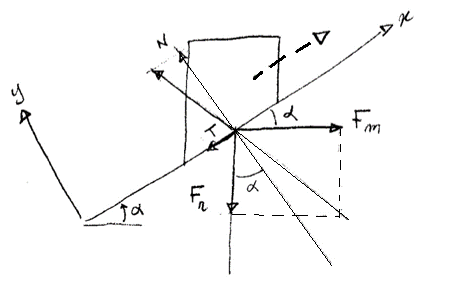
\includegraphics[width=.95\textwidth]{chapter05/Immagine153}
\end{minipage}
\hfill
\begin{minipage}{.5\textwidth}
Prendiamo una semplice massa che si muove su un piano inclinato e che è quindi soggetta ad una forza verticale $F_r$ e una forza motrice $F_m$ per mezzo della quale sale il piano inclinato, diretta lungo il piano orizzontale.

Inoltre tra massa e piano inclinato è presente dell'attrito: la reazione vincolare del piano al contatto con la massa ha una componente normale al piano stesso (N), ma anche una componente che giace sul piano (T) che è la forza d'attrito. Questo porta la risultante alla reazione vincolare a non essere normale al piano inclinato, ma ad opporsi al moto che supponiamo avvenire nella direzione di x positivo.
\end{minipage}

Proviamo a questo punto a scrivere la definizione di rendimento del sistema e a proiettare le equazioni in modo tale da trovare un'espressione che coinvolga anche il coefficiente di attrito nelle condizioni di movimento diretto e (se e come) nelle condizioni di moto retrogrado.

\begin{itemize}
\item Moto diretto: il lavoro resistente è calcolabile come il lavoro che la forza $F_r$ compie man mano che il corpo sale di una quantità positiva $\Delta x$. Analogo per il lavoro motore.
\[\eta = \cfrac{\norma{L_r}}{L_m} = \cfrac{F_r\,\sin{(\alpha)}\,\Delta x}{F_m\,\cos{(\alpha)}\,\Delta x}\]

La relazione che esiste tra le varie forze presenti sul nostro sistema ipotizzando che il sistema sia in una condizione di funzionamento a regime, ovvero sta salendo il piano inclinato con velocità costante:
\[
\begin{cases}
x:\quad\,+\,F_m\,\cos{(\alpha)}\,-\,F_r\,\sin{(\alpha)}\,-\,T = 0\\
y:\quad\,-\,F_m\,\sin{(\alpha)}\,-\,F_r\,\cos{(\alpha)}\,+\,N = 0
\end{cases}
\]
Siamo in possesso anche della relazione fornitaci dal modello Coulombiano di attrito per la quale la componente tangenziale T è proporzionale alla componente normale N, tramite un coefficiente di attrito cinetico (in quanto il sistema è in movimento):
\[T = f\,N\]
Prendiamo ora le due equazioni di bilancio dell'energia e moltiplichiamo la prima per il $\sin{(\alpha)}$ e la seconda per il $\cos{(\alpha)}$, ottenendo:
\[
\begin{dcases}
F_m\,\sin{(\alpha)}\,\cos{(\alpha)}\,-\,F_r\,\sin^2{(\alpha)}\,-\,T\,\sin{(\alpha)}=0\\
-\,F_m\,\cos{(\alpha)}\,\sin{(\alpha)}\,-\,F_r\,\cos^{(\alpha)}\,+\,N\,\cos{(\alpha)} = 0
\end{dcases}
\]
Ne facciamo la somma membro a membro, ottenendo:
\begin{gather*}
-\,F_r\,-\,T\,\sin{(\alpha)}\,+\,N\,\cos{(\alpha)} = 0\\
\begin{dcases}
F_r = N\,(\cos{(\alpha)}\,-\,f\,\sin{(\alpha)})\\
F_m = N\,(\sin{(\alpha)}\,+\,f\,\cos{(\alpha)})
\end{dcases}
\end{gather*}
Calcoliamo il rapporto:
\[\cfrac{F_r}{F_m} = \cfrac{\cos{(\alpha)}\,-\,f\,\sin{(\alpha)}}{\sin{(\alpha)}\,+\,f\,\cos{(\alpha)}}\]
Tale rapporto, se ricordiamo l'espressione trovata per il rendimento, è il rapporto che caratterizza il rendimento stesso.
\[\eta = \cfrac{\norma{L_r}}{L_m} = \cfrac{F_r\,\sin{(\alpha)}\,\Delta x}{F_m\,\cos{(\alpha)}\,\Delta x} = \cfrac{\cos{(\alpha)}\,-\,f\,\sin{(\alpha)}}{\sin{(\alpha)}\,+\,f\,\cos{(\alpha)}}\,\cdot\cfrac{\sin{(\alpha)}}{\cos{(\alpha)}} \]
\item Moto retrogrado: 

\begin{minipage}{.5\textwidth}
\centering
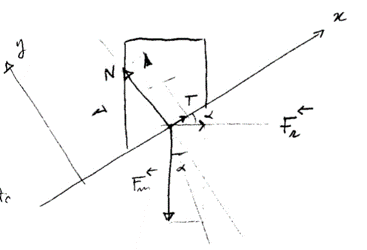
\includegraphics[width=.95\textwidth]{chapter05/Immagine154}
\end{minipage}
\hfill
\begin{minipage}{.5\textwidth}
Vediamo ora le condizioni del nostro sistema in moto retrogrado. Dal disegno del sistema possiamo osservare che la massa è posizionata sul piano inclinato, soggetto a forze orizzontali e verticali.

Il ruolo della forza verticale e della forza orizzontale ora è invertito rispetto al moto diretto: la forza verticale $\ret{F_m}$ diventa la forza motrice in quanto è quella che promuove la discesa del corpo sul piano inclinato (movimento in direzione opposta all'asse x), la forza orizzontale che prima applicavamo per far salire la massa ora diventa la forza resistente $\ret{F_r}$, dalla quale possiamo trarre lavoro utile per l'utenza di questo sistema.
\end{minipage}

Osserviamo che si suppone che il corpo stia scendendo con velocità costante lungo il piano inclinato e di conseguenza la forza di attrito T è diretta in verso positivo rispetto all'asse x, in quanto si sta opponendo alla discesa del corpo lungo il piano inclinato.

Il rendimento in questo senso è pari a:
\[\ret{\eta} = \cfrac{\norma{\ret{L_r}}}{\ret{L_m}}=\cfrac{\ret{F_r}\,\cos{(\alpha)}\,\Delta x}{\ret{F_m}\,\sin{(\alpha)}\,\Delta x}\]
Scriviamo le equazioni di equilibrio del sistema:
\[
\begin{dcases}
x:\quad + \ret{F_r}\,\cos{\alpha}\,+\,T\,-\,\ret{F_m}\,\sin{\alpha} = 0\\
y:\quad + N\,-\,\ret{F_m}\,\cos{\alpha}\,-\,\ret{F_r}\,\sin{\alpha}=0
\end{dcases}
\]
Analogamente al caso precedente possiamo scrivere T = f N e applicando considerazione analoghe ricavare il rapporto
\[\cfrac{\ret{F_r}}{\ret{F_m}}=\cfrac{\sin{\alpha}\,-\,f\,\cos{\alpha}}{\cos{\alpha}\,+\,f\,\sin{\alpha}}\]
che sostituita nell'espressione del rendimento retrogrado:
\[\ret{\eta} = \cfrac{\sin{\alpha}\,-\,f\,\cos{\alpha}}{\cos{\alpha}\,+\,f\,\sin{\alpha}}\,\cdot\,\cfrac{\cos{\alpha}}{\sin{\alpha}}\]
\end{itemize}

\subsection{Equivalenza dinamica di membri rigidi}

Sempre nell'ambito dell'analisi dinamica di sistemi ad 1 G.d.L. ci occupiamo dell'equivalenza dinamica di corpi rigidi.

Due corpi rigidi sono diamicamente equivalenti  se soggetti all'applicazione dello stesso sistema di forze si comportano in modo identico.

È utile in molte applicazioni poter scrivere le equazioni del moto di un sistema rigido in termini di sistema equivalente, quindi poter realizzare un sistema del tutto equivalente a quello di partenza per il quale però la scrittura delle equazioni del moto risultano semplificate (sta a noi trovare strategie di equivalenza più indicate per semplificare il sistema).

Dal punto di vista dinamico l'identità del comportamento tra due sistemi diversi è garantita dal fatto che quantità di moto e momento della quantità di moto siano del tutto uguali: solo in questo caso siamo assolutamente sicuri che il sistema equivalente lo sia veramente, nel senso che si comporti allo stesso modo del sistema di partenza sotto l'effetto di qualsiasi sistema di forze e momenti.

Ci occupiamo di sistemi piani, ovvero la cui dinamica è descritta dal moto in un piano: il problema si può formulare in due dimensioni.

Partiamo dalla formulazione più generale in 3 dimensioni e, in questo caso, la quantità di moto di un sistema piano (xy) proiettata nel S.d.R. fisso si può scrivere come:
\[\leftidx{^f}{\B{Q}} = m\,\,\leftidx{^f}{\B{\dot{x_G}\\\dot{y_G}\\0}}\]
Scriviamo ora il momento della quantità di moto, una volta scelto come polo (per comodità) il centro di massa del corpo:
\[\leftidx{^m}{\B{K_G}} = \leftidx{^m}{\M{I_G}}\,\,\leftidx{^m}{\B{0\\0\\\omega_z}} = \leftidx{^m}{\B{-I_{Gxz}\,\omega_z\\-I_{Gyz}\,\omega_z\\I_{Gzz}\,\omega_z}}\]
Osserviamo che se l'asse z è un'asse principale d'inerzia le prime due componenti sono nulle e quindi l'unica equazione che rimane è la terza che chiama in causa la terza componente della quantità di moto.

Se i due  momenti d'inerzia $I_{Gxz}$ e $I_{Gyz}$ non fossero nulli sono necessari due momenti lungo l'asse x e y della terna mobile per mantenere il sistema in moto piano (ad esempio un vincolo).

Possiamo quindi concludere che l'equivalenza dinamica di due sistemi è garantita da stessa massa, posizione del centro di massa e dal momento d'inerzia attorno all'asse ortogonale al piano del moto. Scriviamo ora le equazioni che ci garantiscono l'equivalenza dinamica di due sistemi: supponiamo di avere un sistema di massa m, di posizione del centro di massa ($x_G, y_G$) e momento d'inerzia attorno all'asse z baricentrico $I_{Gzz}$.

Possiamo pensare che la sua dinamica sia equivalente a quella di una distribuzione di masse che però soddisfi l'equivalenza delle grandezze appena elencate.
\[
\begin{cases}
\sum_i m_i = m\\
\sum_i m_i\,x_i = m\,x_G = 0 \qquad\text{se terna è baricentrica (mobile)}\\
\sum_i m_i\,y_i = m\,y_G = 0 \qquad\text{se terna è baricentrica (mobile)}\\
\sum_i m_i\,(x_i^2\,+\,y_i^2) = I_{Gzz}
\end{cases}
\]
Osserviamo che abbiamo potuto scrivere un sistema di 4 equazioni: quindi volendo abbiamo la possibilità di trovare 4 incognite. Il primo esempio che possiamo fare è che, fissando le posizioni x,y di 4 masse, è possibile ricavare i valori delle masse che rendono tale distribuzioni di corpi equivalente a quella di partenza.

In alternativa potremmo allineare tutte le masse lungo un'asse baricentrico (ad esempio x), in questo modo tutte le coordinate y delle masse sono nulle e, essendo la terza equazione identicamente soddisfatta, mi permette di trovare tre valori di massa che garantisca l'equivalenza del sistema.

\begin{center}
{\scshape{\bfseries Esempio n.1: biella}}
\end{center}

\begin{minipage}{.5\textwidth}
\centering
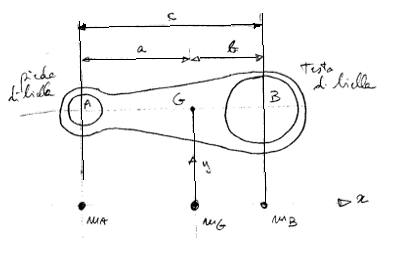
\includegraphics[width=.95\textwidth]{chapter05/Immagine155}
\end{minipage}
\hfill
\begin{minipage}{.5\textwidth}
Prendiamo un corpo rigido esteso, ad esempio la biella di un motore a combustione interna, e ci chiediamo se possiamo scrivere un sistema dinamicamente equivalente che semplifichi la scrittura delle equazioni del moto della dinamica di questo sistema.

Ipotizziamo che il moto avvenga in un sistema piano e scegliamo tre masse localizzate ne punto A,B e G per descrivere un sistema dinamicamente equivalente, allineate lungo l'asse baricentrico.

Le uniche tre incognite che rimangono, avendo scelto la posizione delle tre massse, sono i valori stessi delle masse ($m_A, m_B, m_G$).
\end{minipage}

Scriviamo le tre equazioni di equivalenza:
\[
\begin{dcases}
m_A + m_B + m_G = m\\
-\,a\,m_A\,+\,b\,m_B = 0\\
a^2\,m_A\,+\,b^2\,m_B = I_{Gzz}
\end{dcases}
\]
Il sistema ottenuto è un sistema di tre equazioni in tre incognite che risolto permette di trovare i valori delle tre masse:
\[
m_A = \cfrac{I_{Gzz}}{a\,c}\qquad;\qquad m_B = \cfrac{I_{Gzz}}{b\,c}\qquad;\qquad m_G = m\,-\,m_A\,-\,m_B
\]
Ogni volta che in un qualunque meccanismo ci sia una biella in moto piano possiamo sostituirla con tre masse localizzate nei punti A,B e G. Tale semplificazione è particolarmente efficace in quanto le masse A e B sono posizionate nelle coppie rotoidali e quindi la descrizione del loro moto è particolarmente semplice, mentre il moto del punto G va per forza calcolato.

Per questo stesso sistema possiamo sceglierlo con un sistema dinamicamente equivalente che è formato da solo due masse ($m_A$ e $m_B$) che risulteranno diverse da quelle trovate precedentemente e da un momento di inerzia puto ($I_0$), che è un momento d'inerzia fittizio la cui proprietà è quella di far tornare la dinamica complessiva del sistema equivalente con quella del sistema di partenza.

Sciviamo le equazione di equivalenza dinamica:
\[
\begin{dcases}
m_A\,+\,m_B = m\\
-\,a\,m_A\,+\,b\,m_B = 0\\
a^2\,m_A\,+\,b^2\,m_B\,+I_0=I_{Gzz}
\end{dcases}
\]
Anche questo sistema ha tre equazioni in tre incognite:
\[
m_A = m\,\cfrac{b}{c}\qquad;\qquad m_B = m\,\cfrac{a}{c}\qquad;\qquad I_0 = I_{Gzz}\,-\,m\,a\,b
\]
Questo momento d'inerzia ha un significato matematico e fisico in quanto riequilibria la dinamica del sistema rispetto al sistema di partenza tant'è che tale momento d'inerzia può, in principio, anche essere negativo.

Ogni qualvolta scriveremo l'equazione di Eulero della distribuzione di masse equivalente dovremmo ricordarci di legare la dinamica rotazionale della biella descritta semplicemente dalle due masse con la presenza di un momento d'inerzia $I_0$

\section{Lezione 08-04 -- Daniele Bortoluzzi}

\subsection{Irregolarità e stabilità del moto}

Sempre nell'ambito dell'analisi dinamica di sistema ad 1 G.d.L. affrontiamo una problematica piuttosto comune nelle macchine e nei meccanismi che è la condizione di funzionamento di un sistema descritto da 1 G.d.L.

L'esempio che viene proposto è l'accoppiamento motore-utilizzatore.

Questo sistema è piuttosto semplice in termini di descrizione della sua dinamica in quanto avendo un unico grado di libertà è possibile scriverla con un'unica equazione differenziale però è un caso di studio particolarmente utile e frequente nell'ambito dei meccanismi.

Riprendiamo dunque l'equazione differenziale che genericamente descrive la dinamica di un sistema ad 1 G.d.L.
\[I^*(q)\,\ddot{q}\,+\,\cfrac{1}{2}\,\td{I^*}{q}\,\dot{q}^2 = Q^*\]
Questa equazione differenziale richiede il calcolo del momento d'inerzia ridotto I* e del momento esterno ridotto Q* equivalente a tutte le azioni esterne al meccanismo proiettate lungo la coordinata generalizzata q.

Tale sistema può avere diverse condizioni di funzionamento che dipendono dalla sua natura che dalle condizioni di funzionamento (aka forze e momenti a lui applicati): il primo tipo di condizioni di funzionamento per un sistema di questo tipo sono quelle di \emph{regime assoluto}.

Un sistema ad 1 G.d.L. è in regime assoluto se tutte le velocità dei diversi membri sono costanti nel tempo; questa definizione ci fa capire che è una condizione piuttosto particolare che non è detto si possa realizzare per tutti i meccanismi: ad esempio il meccanismo di spinta (per la descrizione di un compressore volumetrico), se anche la manovella in moto con velocità angolare costante non è vero che gli altri membri del meccanismo sono mantenuti con velocità costante.

Se noi utilizziamo l'equazione differenziale per capire quali sono possibili condizioni di funzionamento di un meccanismo in regime assoluto, ricordando che il momento d'inerzia generalizzato è un momento di'inerzia tale per cui produce un'energia cinetica equivalente del sistema ridotto rispetto al sistema reale e che il momento generalizzato è il momento equivalente che applicato al sistema semplificato esercita la stessa potenza delle azioni effettivamente presenti sul sistema reale, dovremmo imporre $\ddot{q} = 0$.
\[\cfrac{1}{2}\,\td{I^*}{q}\,\dot{q}^2=Q^*\]
Una possibile condizione che verifica tale equazione è che $I^* = cost.$ e che $Q^* = 0$.

L'equazione sotto tale ipotesi è verificata sotto ogni configurazione e abbiamo una condizione di regime assoluto.

Cosa significa che $I^*$ sia costante? Significa che, presa la sua espressione, dovremmo garantire che non vari nel tempo e non vari rispetto alla configurazione.

L'espressione di I* è
\[I^* = \sum_{i=1}^n\,(m_i\,\tau_{xi}^2\,+\,m_i\,\tau_{yi}^2\,+\,I_i\,\tau_{\theta i}^2)\]
La sommatoria è la somma di termini che prevedono massa per il quadrato dei rapporti di velocità tra coordinata generalizzata e velocità del centro di massa del corpo i-esimo e il momento d'inerzia del corpo i-esimo che moltiplica il rapporto di velocità tra la sua rotazione e la coordinata generalizzata. È possibile che tale momento d'inerzia ridotto sia costante se, ad esempio, tutti i rapporti di velocità siano costanti. Questo, tuttavia, non è sempre possibile.\newline

L'altra condizione necessaria è che Q* = 0, ovvero che non ci siano forze nette che agiscono sul nostro sistema (o sono tutte nulle o tutte le forze attive compensano in ogni istante e in ogni configurazione quelle dissipative). Anche questa situazione non è detto che sia verificata per il generico meccanismo.\newline

Premesso ciò per il regime assoluto, che risulta piuttosto restrittivo per il funzionamento di un meccanismo definiamo un nuovo tipo di regime: \emph{il regime periodico}. In esso viene a cadere la richiesta che le velocità di tutti i membri siano costanti nel tempo e ciò che si richiede è che vi sia una certa regolarità, cioè che le velocità di tutti i membri, se non costanti, siano almeno periodiche con periodo pari a T.

Sotto queste ipotesi definiamo una grandezza utile per caratterizzare la natura di variabilità del regime nelle condizioni di periodicità, che risulta essere il valore medio della coordinata libera q:
\[\dot{q}_{med} = \cfrac{1}{T}\,\int_{t_0}^{t_0\,+\,T}\,\dot{q}(t)\,dt\]
Questa definizione non dipende dalla scelta dell'istante $t_0$.

La grandezza derivata dalla definizione di $\dot{q}_{med}$ è il \textbf{Grado di irregolarità periodica}, che quantifica quanto è irregolare il nostro moto prendendo come riferimento il regime assoluto che ha la regolarità più alta:
\[\delta = \cfrac{\dot{q}_{max}\,-\,\dot{q}_{min}}{\dot{q}_{med}}\]
 Tanto maggiore è $\delta$ quanto più è irregolare il moto.
 
L'irregolarità eccessiva del regime periodico può causare alcuni problemi, e sono riconducibili a tre principali problematiche:
\begin{itemize}
\item Un'elevata irregolarità è associata a elevate accelerazioni (lineari e angolari) dei membri del meccanismo, che comportano elevati carichi inerziali agenti sul meccanismo. In condizioni di funzionamento reali significa sollecitare eccessivamente le coppie cinematiche che assemblano il meccanismo.
\item Innesco di oscillazioni dovute ad elevate irregolarità. I carichi inerziali che ne conseguono, in presenza, di flessibilità di organi e accoppiamenti (cedevolezze distribuite o localizzate nel meccanismo), possono innescare oscillazioni e vibrazioni dei membri, le quali possono costituire una non idealità di funzionamento (si discosta dal funzionamento previsto in fase di progettazione), ma anche mettere a repentaglio l'integrità.
\item Un'elevata irregolarità del meccanismo può mettere a repentaglio la qualità stessa del compito che la macchina sta svolgendo.
\end{itemize}

Vengono proposti alcuni esempi di gradi di irregolarità ($\delta$) che siano tollerati in diverse applicazioni:

\begin{itemize}
\item macchine sollevamento, pompe e ventilatore \hfill 1/20 --- 1/30
\item macchine per la tessitura o lavorazione carta \hfill 1/50 --- 1/100
\item moto di automobili \hfill 1/100 --- 1/200
\item alternatori \hfill 1/300
\end{itemize}

Se l'andamento della forma d'onda che descrive la velocità della coordinata generalizzata non è troppo assimetrico è spesso comodo scrivere il valore della velocità media come la media tra il massimo e il minimo della derivata:
\[\dot{q}_{med} \approx \cfrac{\dot{q}_{max}\,+\,\dot{q}_{min}}{2}\]

Possiamo ora studiare più a fondo il problema della regolarità di un meccanismo andando a studiare come un meccanismo si comporta in regime periodico.

Supponiamo che le leggi orarie della coordinata libera e delle sue derivate siano note (ad esempio perché abbiamo risolto le equazioni differenziali o perché abbiamo misurato l'andamento temporale di queste tre grandezze), supponiamo anche di conoscere il momento d'inerzia ridotto ($I^*(q(t)) = I^*(t)$).

Una volta noto I*(t) e la derivata temporale della coordinata libera possiamo calcolare l'andamento temporale dell'energia cinetica come:
\[E_c(t) = \cfrac{1}{2}\,I^*(q(t))\,\dot{q}(t)^2\]
\begin{minipage}{.5\textwidth}
Possiamo a questo punto diagrammare l'andamento dell'energia cinetica e il momento d'inerzia ridotto in funzione del tempo: il loro andamento sarà ciclico del tipo rappresentato in figura di periodo uguale a quello della coordinata libera (o eventualmente un suo sottomultiplo).

Il motivo per cui sono stati rappresentati nel modo rappresentato è perché vogliamo intersecare le due curve in un luogo dei punti (diagramma parametrico nel tempo) in cui abbiamo in ascissa il momento d'inerzia ridotto e in ordinata l'energia cinetica.

In questo caso, gli andamento periodici generano una curva chiusa nel diagramma parametrico che può essere interpretata come una ellisse percorsa in senso orario. 
\end{minipage}
\hfill
\begin{minipage}{.5\textwidth}
\centering
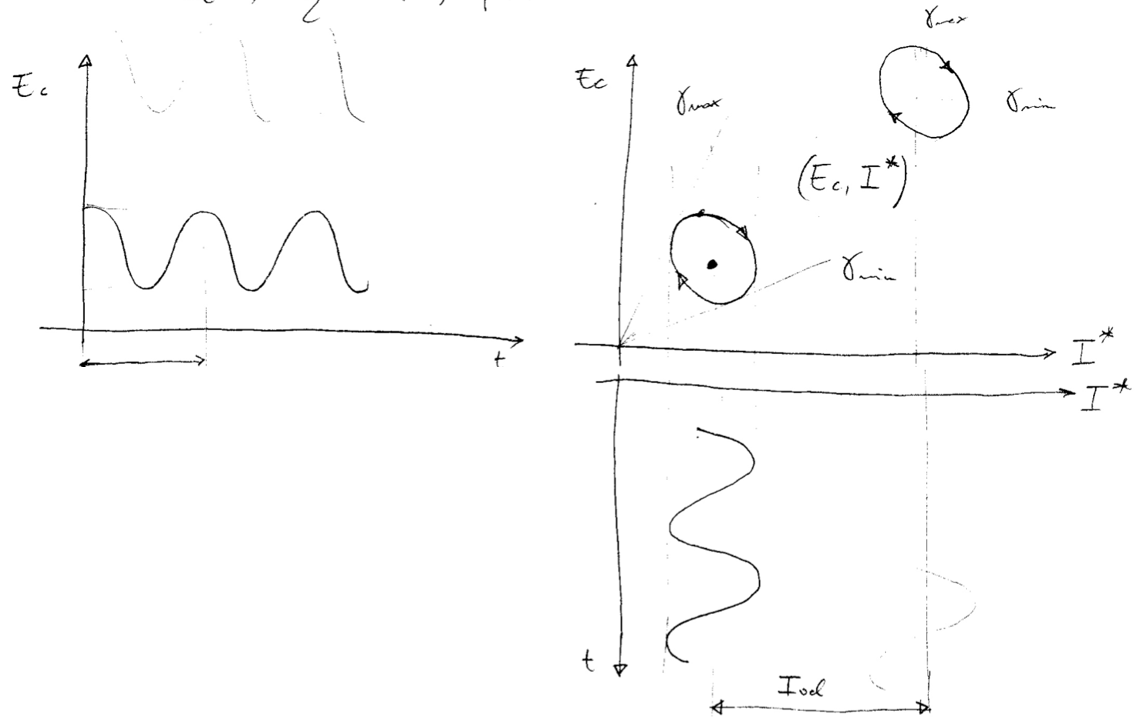
\includegraphics[width=.95\textwidth]{chapter05/Immagine156}
\end{minipage}

Questo diagramma sintetizza in un unico grafico le due grandezze principali e tramite questo possiamo calcolare la grandezza $\gamma$, che altro non è che l'angolo sotteso dalla congiungente del generico punto dl grafico con l'origine verso l'asse orizzontale.
\[\tan{\gamma} = \cfrac{E_c(t)}{I^*(t)} = \cfrac{\cfrac{1}{2}\,I^*(q(t))\,\dot{q}(t)^2}{I^*(q(t))} = \cfrac{1}{2}\,\dot{q}(t)^2\]
Dato un generico punto ($E_c(t),I^*(q(t))$), la tangente dell'angolo ($\gamma$) è indicativa della metà della velocità al quadrato della coordinata libera, nell'istante che compete al punto considerato.

Richiamando la definizione di $\delta = \cfrac{\dot{q}_{max}\,-\,\dot{q}_{min}}{\dot{q}_{med}}$, essendo $\dot{q}$ una grandezza legata alla pendenza della congiungente del punto con l'origine possiamo associare la pendenza di questa retta con la velocità.

Data un'orbita, come quella descritta nel diagramma in alto a destra, le velocità massima e minima saranno raggiunti nei punti in cui la pendenza della retta è massima o minimo ($\gamma_{max},\gamma_{min}$).

La differenza delle due pendenza è un indicatore dell'escursione di velocità che si ha nel funzionamento della macchina per cui l'orbita è stata tracciata, di conseguenza possiamo già visualizzare il grado di regolarità di una macchina andando a osservare l'escursione di $\gamma$ rispetto al $\gamma_{med}$, ovvero la pendenza della retta passante per l'origine e il centro dell'orbita che descrive il ciclo del meccanismo di riferimento.

Quale può essere una strategia per migliorare la regolarità di questa macchina osservando il suo comportamento nel diagramma di interesse?

La soluzione che è spesso adottata è quella di aggiungere un volano all'albero motore, mantenendo il meccanismo così com'è, in questo modo si aggiunge un momento d'inerzia che va ad alterare i due diagrammi di momento d'inerzia ridotto e energia cinetica.

Proviamo a osservare come sia possibile quantificare il beneficio dell'introduzione di un momento d'inerzia costante sul nostro sistema:

Calcoliamo in primo luogo l'andamento dell'energia cinetica del nostro meccanismo applicando il teorema delle forze vive: sappiamo, infatti, che la variazione di energia cinetica è pari al lavoro esercitato da tutte le azioni esterne al sistema (che sono descritte da Q*) tra due configurazioni generiche.
\[\int_{q_1}^{q_2}\,Q^*(q)\,dq = E_{C2}\,-\,E_{C1}\]
Possiamo sfruttare questa equazione, in cui l'energia cinetica è scritta in forma di funzione integrale, per trovare quando essa sia stazionaria:
\[\td{}{q}\,\int_{q_1}^{q_2}\,Q^*(q)\,dq = Q^* = Q^*_m\,+\,Q^*_r\,+\,Q^*_P = 0\]
Si osserva infatti che la funzione integranda contiene i contributi delle forze/coppie motrici, resistenti e dissipative.

Quando tale equazione sarà  pari a zero si potrà osservare un punto di massimo relativo o minimo relativo.

Chiamiamo queste configurazioni Q in cui l'energia cinetica assume valore massimo o minimo rispettivamente $q_{max}$ e $q_{min}$.

Possiamo a questo punto riscrivere che:
\[\int_{q_{min}}^{q_{max}}\,Q^*(q)\,dq = E_{c\,max}\,-\,E_{c\,min} = \cfrac{1}{2}\,I^*(q_{max})\,\dot{q}_{max}^2\,-\,\cfrac{1}{2}\,I^*(q_{min})\,\dot{q}_{min}^2\]
Supponiamo ora che la nostra espressione del momento d'inerzia ridotto contenga un termine costante aggiuntivo che abbiamo introdotto nel sistema aggiungendo un volano all'albero motore. Esprimeremo questo concetto nel seguente modo:
\[=\cfrac{1}{2}\,(I^*_{cost}\,+\,I^*_{var}(q_{max}))\,\dot{q}_{max}^2\,-\,\cfrac{1}{2}\,(I^*_{cost}\,+\,I^*_{var}(q_{min}))\,\dot{q}_{min}^2\]
Osserviamo come da questa relazione sia possibile estrarre una equazione significativa del grado di regolarità del meccanismo in presenza del volano aggiuntivo.

Definiamo $\Delta$ la quota di escursione di energia cinetica associato all'inerzia costante aggiunta al sistema, essa è possibile calcolarla come:
\[\Delta = \cfrac{1}{2}\,I^*_{cost}\,(\dot{q}_{max}^2\,-\,\dot{q}_{min}^2)= \int_{q_{min}}^{q_{max}}\,Q^*(q)\,dq\,-\,\cfrac{1}{2}\,I^*_{var}(q_{max})\,\dot{q}_{max}^2\,-\,\cfrac{1}{2}\,I^*_{var}(q_{min})\,\dot{q}_{min}^2 \]
 Ricordiamo che esiste l'espressione approssimata della $\dot{q}_{med} \approx \cfrac{\dot{q}_{max}\,-\,\dot{q}_{min}}{2}$ e, noto ciò, possiamo scrivere il grado di regolarità del nostro sistema in presenza del momento di inerzia aggiuntivo costante:
 \[\delta = \cfrac{\dot{q}_{max}\,-\,\dot{q}_{min}}{\dot{q}_{med}} \approx \cfrac{(\dot{q}_{max}\,-\,\dot{q}_{min})}{\dot{q}_{med}} \cdot\cfrac{(\dot{q}_{max}\,+\,\dot{q}_{min})}{2\,\dot{q}_{med}} = \cfrac{\dot{q}^2_{max}\,-\,\dot{q}^2_{min}}{2\,\dot{q}^2_{med}} = \cfrac{\Delta}{I^*_{cost}\,\dot{q}^2_{med}}\]
Questa relazione quantifica il grado di regolarità del sistema una volta che sia stato aggiunto l'inerzia costante e mostra come un'aumento di tale valore aggiuntivo porti ad una diminuzione del grado di irregolarità del nostro sistema.

La cosa può essere visualizzata nel diagramma ($I^*, E_c$), osservando che aggiungendo un'inerzia costante, i grafici dell'energia cinetica nel tempo e del momento d'inerzia ridotto nel tempo vengono aumentati e, di conseguenza, la traiettoria chiusa generata nel piano si allontana dall'origine mantenendo il suo centro sulla stessa retta che passa per l'origine e il centro della traiettoria originale (poiché $\dot{q}_{med}$ non viene alterato). Tuttavia la nuova orbita descritta vedrà le due pendenza ($\gamma_{max}$ e $\gamma_{min}$) si saranno avvicinate alla retta di pendenza $\gamma_{med}$ il ché implica un aumento del grado di regolarità del nostro sistema.

Ovviamente le controindicazioni di questa scelta sono legate al fatto che il sistema soggetto alle stesse azioni motrici e resistenti impiegherà più tempo ad arrivare a regime e richiederà dei tempi transitori più lunghi per arrivare alla condizione di funzionamento presa a riferimento nel grafico.

Inoltre quello che è utile al fine di questo calcolo è l'inerzia del volano ridotta alla coordinata di riferimento q; in particolare in presenza di diversi alberi che hanno diverse velocità di rotazione è opportuno installare, se possibile, il volano sull'albero di velocità angolare maggiore dal momento che l'inerzia ridotta all'albero di riferimento è il momento del volano moltiplicato per il rapporto di velocità al quadrato:
\[I^*_{vol} = I_{vol}\,\tau^2\]
In questo modo l'installazione del volano sull'albero con velocità angolare maggiore beneficia in termini quadratici del rapporto di velocità tra l'albero in cui è installato e l'albero la cui rotazione è la coordinata generalizzata di riferimento per il calcolo.

\subsection{Stabilità del funzionamento delle macchine}

C'è un altro aspetto interessante che caratterizza le condizioni di funzionamento di un sistema meccanico in cui accoppiamo un motore ad un sistema resistente: la stabilità del funzionamento del sistema accoppiato.

Supponiamo di avere un diagramma in cui è presente, in funzione della derivata della coordinata generalizzata ($\dot{q}$), l'andamento del momento generalizzato motore $\mathbf{Q^*_m}$, messo a disposizione dal motore alla coordinata $\dot{q}$, e resistente $\mathbf{Q^*_r}$, che l'utenza richiede alla coordinata generalizzata q.

\begin{center}
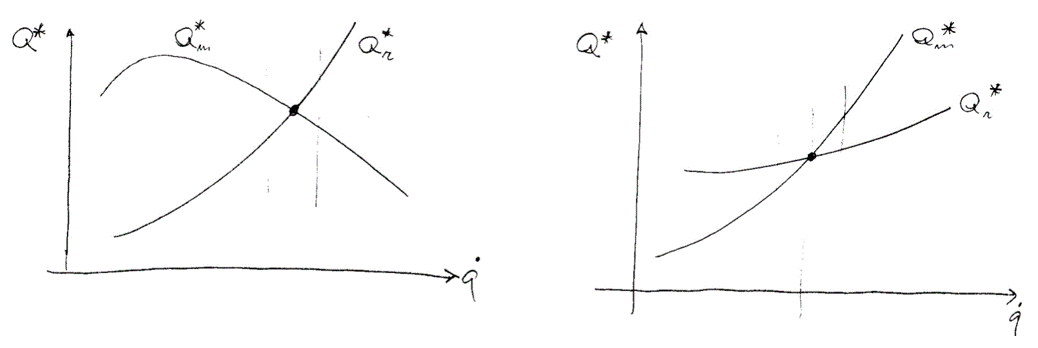
\includegraphics[width=.8\textwidth]{chapter05/Immagine157}
\end{center}

Si possono presentare diversi casi:
\begin{itemize}
\item Il momento motore è una funzione decrescente della coordinata $\dot{q}$, perché, ad esempio, è un motore elettrico o a combustione interna in regime di funzionamento normale, e che l'andamento del momento resistente sia una funzione crescente come quella diagrammata a sinistra.

Il punto di funzionamento in cui il sistema funzionerà con velocità angolare costante è individuato dall'intersezione delle due curve in cui il momento motore eguaglierà quello resistente.

Se le condizioni del nostro sistema sono quelle rappresentate in figura, ovvero in cui la pendenza della curva motrice è negativa e la pendenza della curva resistente è positiva, vale la disuguaglianza:
\[\td{Q_m^*}{\dot{q}}\,<\,\td{Q_r^*}{\dot{q}}\]
Si dice che questa configurazione di funzionamento è una configurazione stabile, e di conseguenza il punto di funzionamento è stabile, in quanto, immaginando di perturbarlo, osserviamo che il sistema reagisce cercando di portare il punto di funzionamento al punto di riferimento

Entro i limiti di mantenimento della precedente disuguaglianza il sistema tende ad opporsi a qualsiasi perturbazione che alteri il funzionamento dell'accoppiamento motore-carico caratterizzato da quel punto di equilibrio
\item Un'altra situazione è descritta dalla disuguaglianza opposta:
\[\td{Q^*_m}{\dot{q}}\,>\,\td{Q_r^*}{\dot{q}}\]
Le due curve possono, ad esempio, essere entrambe crescenti, dove tuttavia la curva motrice ha una pendenza maggiore di quella resistente nell'intorno del punto di riferimento in cui il sistema è in equilibrio.

Immaginando di perturbare il sistema nell'intorno del punto di equilibrio, osserviamo una situazione opposta a quella che si verificava nel caso precedente, per questa ragione tale condizione/sistema è detto instabile.

L'allontanamento dal punto di equilibrio crea uno squilibrio di azioni che promuove l'allontanamento stesso dal punto di riferimento, questo finché si verificheranno le condizioni descritte dall'uguaglianza precedentemente presentata.
\end{itemize}

\subsection{Componenti meccanici: le coppie cinematiche}

Le coppie cinematiche costituiscono degli elementi particolarmente critici dei meccanismi, sono infatti quegli organi che garantiscono l'accoppiamento tra due organi meccanici in movimento relativo, e di conseguenza il loro comportamento deve avvicinarsi il più possibile a quello delle coppie ideali, ovvero garantire il vincolo relativo tra i membri che sono componenti del meccanismo assicurando che la cinematica e la dinamica dello stesso si svolgano secondo le prestazioni di progetto.

Abbiamo già visto che le coppie cinematiche si possono classificare secondo vari criteri:
\begin{itemize}
\item Classificazione sulla base del tipo di moto relativo che si realizza all'accoppiamento. Esistono, infatti:
\begin{enumerate}
\item \textbf{Coppie a strisciamento} quando le superfici relative dei due membri vincolati reciprocament avviene per strisciamento, ovvero con parti direttamente a contatto e con velocità relative diverse da zero.

Questo può causare una serie di problematiche che vengono limitate dalla presenza di lubrificante: interponendo tra le superfici in moto relativo un fluido con opportune proprietà. Talvolta questo non si fa e si progettano le superfici in maniera tale che possano sostenere le condizioni di esercizio anche in assenza di lubrificante.
\item \textbf{Coppie a rotolamento}: il moto relativo tra gli elementi cinematici della coppia è mediato dalla presenza di corpi che rotolando permettono di mantenere in movimento le superfici relative in assenza (idealmente) di strisciamento.

Quindi, si frappongo tra gli elementi cinematici della coppia dei corpi volventi come, ad esempio, sfere, rulli, coni, etc... e questo comporta una serie di vantaggi, ma anche delle implicazioni costruttive e di prestazione della coppia cinematica.
\item \textbf{Coppie speciali}: realizzano il moto relativo tra i due organi che devono essere vincolati reciprocamente mediante corpi elastici.

Queste hanno una serie di vantaggi legati all'assenza di discontinuità di materiale (o comunque è presente unicità di comportamento) tra i due corpi vincolati, però permettono una mobilità limitata.
\end{enumerate}
\item Classificazione sulla base dei G.d.L. lasciati liberi nel moto relativo tra un corpo e l'altro. Per meccanismi piani esistono:
\begin{enumerate}
\item \textbf{Coppie di classe inferiore} o di classe $c_1$, ad esempio la coppia rotoidale e la coppia prismatica, chiamate in questo modo in quanto permettono una mobilità relativa tra un corpo e l'altro di 1 G.d.L. (basta una coordinata per descrivere la posizione di un corpo rispetto all'altro).
\item \textbf{Coppie di classe superiore} o di classe $c_2$, ad esempio la coppia a camma, che permettono una mobilità relativa dei due corpi vincolati di 2 G.d.L. (sono necessarie 2 coordinate per descrivere la configurazione relativa).
\end{enumerate}
\item Classificazione geometrica, che distingue se i contatti degli elementi cinematici della coppia sono lineari o puntiformi. Si focalizzano sul tipo a livello microscopico del contatto tra gli elementi cinematici. Pensiamo ad esempio il contatto tra un cilindro e un piano che è sostanzialmente un segmento, tra una sfera e un piano c'è un contatto che è idealmente un punto.
\item Classificazione di natura fisico chimica che si focalizza sulla interposizione di un lubrificante di una natura fluida o solida
\item Classificazione dal punto di vista cinematico individuando il tipo di moto relativo tra gli elementi cinematici (strisciamento, rotolamento o presenza di urti).
\end{itemize}

La meccanica del contatto è quella disciplina che si occupa di analizzare come nascono le interazioni reciproche al contatto con due corpi. Ci sono diverse teorie che si applicano a diversi tipi di contatto e in diverse condizioni al contorno, ma c'è una disciplina specifica che si occupa dei fenomeni che avvengono tra superfici in moto relativo e quindi studiano dei modelli che possano descrivere a diversi livelli (da macroscopico a microscopico) come si realizzano le interazioni al contatto tra due corpi.

Tra gli argomenti di interesse che vengono indagati all'interno della \textbf{tribologia} si hanno sia gli studi sull'attrito, ovvero su come nascono e come si comportano le componenti di sforzo di natura dissipativa al contatto tra due superfici in moto relativo, che gli studi sull'usura, ovvero come si generano le particelle di usura e di come le superfici vengano degradate dal proseguire del moto relativo in presenza di specifici carichi tra le superfici in contatto.

Ciò che succede al contatto tra due superfici è un effetto di moltissimi elementi/caratteristiche dei corpi e delle superfici, ad esempio: le proprietà dei materiali che caratterizzano la coppia cinematica sono di fondamentale importanza; si parla dell'effetto dell'elasticità, della plasticità, della curva sforzo-deformazione, dell'isteresi, della durezza, etc...

Tra queste richiamiamo una caratteristica del materiale che è la durezza Brinell, che è una grandezza che caratterizza la durezza del materiale mediante una prova specifica, la quale prevede di forzare una superficie sferica al contatto con una superficie piana; dopo l'applicazione di un carico (forza F) si va a misurare l'area dell'impronta che è rimasta sulla superficie in prova.

La superficie sferica che viene forzata contro la superficie in prova, di conseguenza, lascierà un'impronta che verrà misurata e la durezza Brinell è esattamente il rapporto tra la forza applicata (F) e l'area della superficie dell'impronta che è stata generata. ($HB = F/A$)

Per vari materiali di interesse ingegneristico, per quanto riguarda le coppie cinematiche, una relazione che è piuttosto comune, anche se un po' approssimata, è che la durezza Brinell $HB \approx 3\,\sigma_{ys}$. Questa relazione ci permette di fare calcoli interessanti sui fenomeni che avvengono al contatto tra due superfici.

Ci sono molte altre proprietà fisico-chimiche che vengono coinvolte nel comportamento del contatto tra due superfici, ad esempio:
\begin{itemize}
\item Proprietà termiche: generazione e smaltimento di calore che viene sviluppato localmente al contatto;
\item Proprietà chimiche: capacità di trattenere lubrificanti o alterare o garantire alcune proprietà chimiche superficiali coinvolte nel comportamento delle coppie cinematiche;
\item Rugosità (finitura della superfici), etc...
\end{itemize}

Proviamo ad analizzare al livello microscopico, con un modello molto approssimato, quello che succede al contatto tra due superfici.
\vspace{1mm}

\begin{minipage}{.5\textwidth}
Supponendo di avere due superfici in contatto si può individuare un'area apparente di contatto, che è la superficie nominale interessata dal contatto; tuttavia queste due superfici, dal punto di vista microscopico, non sono superfici piane (nonostante lo possano apparire), ma quello che si realizza è un contatto tra asperità che caratterizzano entrambe le superfici.
\end{minipage}
\hfill
\begin{minipage}{.5\textwidth}
\centering
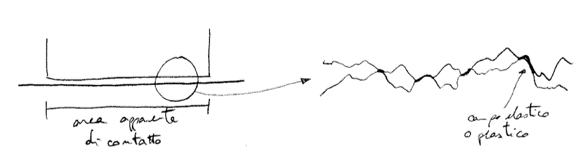
\includegraphics[width=.95\textwidth]{chapter05/Immagine158}
\end{minipage}
\vspace{1mm}

La vera interazione tra le due superfici poste a contatto dipende dalla natura microscopica della finitura delle due superfici coinvolte.

Se guardiamo nel grafico proposto, si osserva che, per loro natura, essendo le superfici reali di natura frattale, l'area reale di contatto è molto minore dell'area apparentemente coinvolta nel contatto: per questo motivo i contatti che sono realizzati a livello microscopico si possono trovare in condizioni locali di sforzo molto maggiore dello sforzo nominale che si può ricavare dal rapporto tra la forza/carico imposto sull'area apparente di contatto.

Quello che succede a livello microscopico può essere una condizione di plasticizzazione anche se la superficie apparente sembra più che sufficiente a garantire un funzionamento in regime elastico del contatto.

\begin{minipage}{.5\textwidth}
Possiamo provare a interpretare i contatti superficiali come una serie di prove Brinell, le quali portano per loro natura il materiale a condizioni di plasticità e quindi in condizioni di subire una deformazione permanente che viene quantificata con l'area A presente nella definizione della durezza stessa.
\end{minipage}
\hfill
\begin{minipage}{.5\textwidth}
\centering
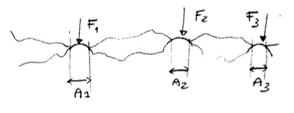
\includegraphics[width=.95\textwidth]{chapter05/Immagine159}
\end{minipage}

Se proviamo a ingrandire la superficie di contatto tra due corpi e interpretare i vari contatti come delle piccole prove Brinell, possiamo scrivere, per ciascuna di esse, che l'area del contatto locale ($A_i$) è pari al rapporto tra la forza esercitata sul contatto locale ($F_i$) e la durezza Brinell (HB).

Le forze che si esercitano al contatto tra ciascuna asperità sono forze più piccole della risultante, tuttavia la loro somma è la forza che, dal punto di vista macroscopico, viene esercitata su un corpo contro l'altro.

Dunque, se scriviamo che l'area locale di contatto è approssimabile come:
\[A_i \approx \cfrac{F_i}{HB}\]
Nell'ipotesi che tutto il materiale sia uniforme e quindi tutte le asperità siano caratterizzate dalla stessa durezza HB, possiamo calcolare l'area reale di contatto come la somma delle singole aree di contatto:
\[A_r \approx \sum_i\,\cfrac{F_i}{HB} = \cfrac{F}{HB}\]
L'area reale si può approssimare come il rapporto tra la forza totale che viene esercitata tra le due superfici e la durezza Brinell; in questo modo si ha una stima dell'area reale di contatto che, secondo questo modello, risulta proporzionale alla forza applicata dall'esterno.

Si tratta chiaramente di un modello approssimato, ma studi più approfonditi confermano che l'area reale di contatto è notevolmente più piccola dell'area apparente fino, ad esempio, ad arrivare a valori di area reale pari a 1/1000 di quella apparente.

Possiamo anche scrivere, osservando la relazione, che l'area reale è il rapporto tra la forza complessivamente applicata e una pressione $P_m$, che altro non è che la pressione a cui corrisponde nel materiale più tenero dell'accoppiamento in esame lo stato triassiale al limite della plasticità.

Tale pressione è grossomodo pari alla durezza Brinell.\newline

Abbiao visto che una possibile classificazione dei contatti è \textbf{di natura geometrica}, il che significa che possiamo caratterizzare i contatti tra due corpi sulla base della natura della superficie di contatto ideale e reale.

Ci sono vari modelli per studiare il contatto da questo punto di vista, ma quello più utilizzato è il \textbf{modello di Hertz} che si preoccupa di determinare stato tensionale e deformazioni dei solidi in prossimità del punto di contatto nell'ipotesi che tali solidi siano omogenei e isotropi, che le deformazioni siano elastiche (nel limite di elasticità lineare del materiale), che le dimensioni dei corpi siano piccole rispetto ai raggi di curvature (ovvero che si abbia un'analisi localizzata al punto di contatto).

Tale teoria permette di:
\begin{enumerate}
\item Descrivere l'andamento delle pressioni (quindi l'andamento locale degli sforzi sulle superfici di contatto);
\item Trovare la geometria delle superfici di contatto;
\item Mettere in relazione tra loro caratteristiche macroscopiche (come la forza risultante al contatto e la deformazione elastica dei corpi).
\end{enumerate}

\begin{center}
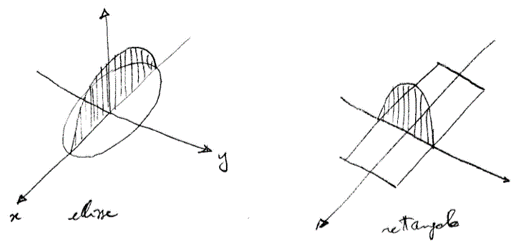
\includegraphics[width=.75\textwidth]{chapter05/Immagine160}
\end{center}

Nell'immagine sono risportati due casi di riferimento: il contatto su una superficie ellittica e rettangolare con l'andamento qualitativo delle pressioni sull'area di contatto.

Ci sono per l'appunto i modelli che descrivono lo stato tensionale in termini di tensore degli sforzi; tuttavia ci basta sapere che alla fine è possibile trovare nelle grandezze di interesse, per quanto riguarda lo studio della coppia cinematica, la relazione tra la forza di contatto e gli assi principali dell'ellisse che descrive l'impronta di contatto in funzione della forza stessa di contatto, dei raggi di curvatura dei corpi posti a contatto, del modulo di elasticità e del modulo di Poisson.

Ad esempio nel caso di un contatto sfera-piano la relazione tra la forza (F) e il cedimento (d) è una relaizone non lineare: si osserva che il comportamento tra forza e deformazione locale è descritto dalla legge 
\[F = c\,\sqrt{d^3}\]
A questo corrisponde un comportamento caratteristico del contatto sfera-piano, che può essere utilizzato per descrivere la pressione di corpi volventi o cuscinetti, non lineare che richiede una serie di strategie per limitarne gli effetti (come ad esempio im precarico dato ai cuscinetti con corpi volventi).\newline

La classificazione dei contatti può avvenire anche sulla base della presenza o assenza di interposizioni di sostanze estranee a quelle dei due elementi cinematici della coppia (classificazione dal punto di vista chimico-fisico).

Distinguiamo dunque tra:
\begin{enumerate}
\item Il \textbf{contatto diretto}, che avviene nominalmente in assenza di interposizione di sostanze estranee. Nonostante questa ssenza di sostanze si possa pensare che sia sempre presente a meno che non si introduca intenzionalmente lubrificante, in realtà non è vero: una superficie metallica è comunque caratterizzata da una serie di strati che separano le due superfici propriamente metalliche, quando esse vengono messe in contatto.

Analizzando dal punto di vista microscopico una superficie metallica partendo dal substrato metallico (dove sono presenti i grani metallici nella loro configurazione nominale) e avvicinandosi alla superficie si osserva uno strato di materiale metallico che è stato incrudito dalla lavorazione metallica che la superficie ha subito.

Le caratteristuche della superficie metalliche vengono alterate rispetto a quello del substrato (lo strato incrudito può essere di uno spesso dell'ordine del micron).

Al di sopra dello strato incrudito è presente, quasi sempre, uno strato di ossido: a causa dell'esposizione all'atmosfera, gran parte dei metalli sviluppa una superficie di ossida di spessore dell'ordine di grandezza del centesimo di micron.

Al di sopra dello strato di ossido molto spesso si osservano altri strati, che sono ad esempio il contaminante (uno strato dell'ordine di grandezza del nanometro, di sostanze contaminanti come grassi o sostanza provenienti dall'atmosfera e dalle manipolazioni subite dal materiale) e gas absorbiti dalla superfici stessa (ossigeno o vapor d'acqua).
\item \textbf{Contatti mediati}, in cui viene intenzionalmente interposto il lubrificante a limitare il contatto tra le due superfici. Il lubrificante ha l'effetto di limitare il più possibile l'interazione tra le due superfici in moto relativo.

Diverse possilbità sono disponibili per la lubrificazione delle superfici in moto relativo: la \textbf{lubrificazione limite}, che si realizza quando il movimento relativo tra le due superfici non riesce a impedire il contatto tra alcune asperità (nonostante questo l'uso del lubrificante riesce a ridurre l'attrito se confrontato con la situazione di contatto diretto); la \textbf{lubrificazione fluida}, che impedisce il contatto tra le superfici.

Per quanto riguarda la lubrificazione fluida esistono due possilbità:
\begin{enumerate}
\item La lubrificazione idrodinamica, in cui lo strato di lubrificante riesce a mantenere separate le due superfici in virtù del moto stesso delle due superfici (il moto relativo delle due superfici promuove la loro separazione grazie alla presenza del lubrificante); 
\item La lubrificazione idrostatica, in cui la separazione tra le due superfici è promossa dall'immissione forzata dell'olio o lubrificante. Il lubrificante viene immesso con una pressione tale da garantire la separazione delle due superfici, limitando (o annullando del tutto) le interazioni indesiderate tra le stesse.
\end{enumerate}
\end{enumerate}

\section{Lezione 15-04 -- Daniele Bortoluzzi}

Proseguiamo a parlare delle coppie cinematiche nell'ambito dei componenti meccanici.

\subsection{Richiamo sui vincoli}

Un vincolo è un dispositivo che limita i G.d.L. di un corpo tramite l'esercizio di forze. Un vincolo ideale, tuttavia, esercita delle forze/azioni anche lungo i G.d.L. che si presuppone siano stati lasciati liberi e questo è legato ai fenomeni di attrito che cerchiamo di formalizzare di seguito:
\vspace{1mm}

\begin{minipage}{.5\textwidth}
\centering
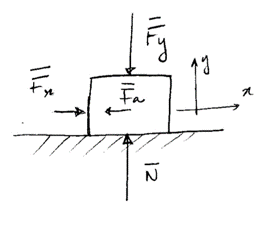
\includegraphics[width=.95\textwidth]{chapter05/Immagine161}
\end{minipage}
\hfill
\begin{minipage}{.5\textwidth}
Consideriamo due corpi a contatto le cui azioni saranno descritte prendendo un S.d.R. i cui assi corrispondono a: \textbf{x} la direzione in cui il corpo dovrebbe essere libero di muoversi, \textbf{y} la direzione vincolata dal vincolo.

Osserviamo che pur essendo il vincolo in grado di equilibrare, mediante la componente N di reazione vincolare, le forze esterne	$\mathbf{F_x}$ e $\mathbf{F_y}$, nella direzione in cui il corpo dovrebbe essere libero di muoversi, il vincolo esercita un'azione/forza non nulla.\newline

Quello che si osserva sperimentalmente è che la componente $F_y$ è equilibrata da N, mentre la presenza di una componente x ($F_x$) non sempre è in grado di causare il movimento del corpo. 
\end{minipage}

Questo è un fenomeno che si realizza a soglia: fintanto che questa componente di forza non supera una certa soglia, il corpo rimane fermo (il vincolo esercita una forza sufficiente a mantenere il corpo in quiete anche lungo la direzione x).

\begin{minipage}{.5\textwidth}

La forza che il vincolo esercita per equilibrare l'azione esterna $F_x$ è detta \textbf{forza d'attrito statico}.

Una volta superato un certo valore soglia, il corpo invece si muove.

Si dice che finché non si raggiunge la condizione di movimento la reazione vincolare che il vincolo esercita non è nota, ed è indeterminata all'interno di un cono, detto \textbf{cono di attrito}, la cui ampiezza è anche definita \textbf{angolo di attrito}.

Ricordiamo che la reazione vincolare finché non vi è movimento è indeterminata nel senso che non sappiamo quale sia la forza esercitata dal vincolo.
\end{minipage}
\hfill
\begin{minipage}{.5\textwidth}
\centering
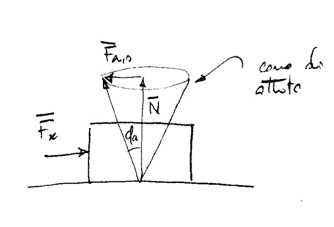
\includegraphics[width=.95\textwidth]{chapter05/Immagine162}
\end{minipage}

Questo fenomeno a soglia si rivela sperimentalmente proporzionale alla componente di reazione vincolare normale (ovvero nella direzione ideale che si sta realizzando), cioé la forza massima che il vincolo può esercitare nella direzione in cui non dovrebbe farlo è proporzionale alla forza che lo stesso vincolo sta esercitando nella direzione ideale di funzionamento del vincolo.

Ha senso dunque definire il \textbf{coefficiente di aderenza} (o attrito statico) $\mathbf{f_a}$, che è calcolato come il rapporto:
\[f_a = \cfrac{F_{a,s}}{N}\]
dove:
\begin{itemize}
\item $F_{a,s}$ è la massima forza che il vincolo può esercitare nella direzione che dovrebbe lasciare libera
\item N è forza che il vincolo esercita nella direzione in cui si presuppone che reagisca
\end{itemize}

Il fenomeno di aderenza descrive il fatto che il corpo e il vincolo rimangono in equilibrio entro le condizioni descritte dal cono di attrito statico.

Un'altra grandezza di interesse è l'angolo di aderenza:
\[\varphi_a = \arctan{\cfrac{F_{a,s}}{N}} = \arctan{f_a}\]

 Quando la soglia di forza è superata, sappiamo che il corpo comincia a muoversi e le condizioni che si realizzano al contatto cambiano: la resistenza che il corpo incontra nella direzione in cui avviene il moto non è più quella che si era realizzata in condizioni statiche. La soglia varcata per produrre il moto del corpo vincolato non è più valida come riferimento per la forza che si oppone al moto.
 
 In particolare, la forza che ora si oppone al moto risulta più bassa della forza di soglia varcata per causare il moto: le condizioni che si hanno in moto relativo sono diverse e richiedono la definizione di un coefficiente di attrito (\textbf{radente o cinetico}) dedicato a questa situazione.
 
 In movimento la $F_a \ne F_{a,s}$, ma è un nuovo valore $F_{a,c} (< F_{a,s})$. Il nuovo coefficiente di \textbf{attrito radente o cinetico} è calcolato come:
 \[f_c = \cfrac{F_{a,c}}{N}\qquad;\qquad f_c < f_a\]
 Sempre relativamente alle condizioni cinetiche (ovvero di strisciamento relativo) definiamo un nuovo angolo di attrito:
 \[\varphi_c = \arctan{\cfrac{F_{a,c}}{N}}=\arctan{f_c}\]
 Possiamo identificare ora due coni che caratterizzano le condizioni di interazione tra corpo e vincolo che risultano essere coassiali (con asse la normale alla superficie di vincolo), e il cono di attrito cinetio è più stretto del cono di attrito statico.
 
 Nelle condizioni cinetiche abbiamo la conoscenza dell'attrito perché sappiamo che questo è esercitato dal vincolo nella direzione opposta al moto, cosa che invece non sapevamo quando il sistema era in equilibrio in quanto non era nota a priori la forza che il vincolo sta esercitando.
 
 In sintesi:
 \vspace{1mm}
 
 \begin{tabular}{llcr}
 In condizioni statiche&:&$F_a \le f_a\,N$&\\
 In condizioni limite&:&$F_{a} = F_{a,s}= f_a\,N$&\\
 In condizioni cinetiche&:&$F_a = F_{a,c} = f_c\,N$&$f_c < f_a$
 \end{tabular}

Motivo per cui può essere utile definire l'angolo di attrito, e non solo il coefficiente di attrito, è mostrato nei tre casi presentati di seguito:
\begin{center}
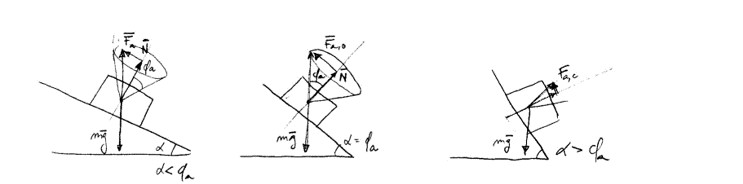
\includegraphics[width=.7\textwidth]{chapter05/Immagine163}
\end{center}

Supponendo di avere un corpo appoggiato su un piano inclinato e al contatto tra i due è presente un certo attrito:
\begin{itemize}
\item Quando l'angolo di inclinazione del piano inclinato è inferiore all'angolo di aderenza osseviamo che l'unica forza esterna presente (la forza peso), giace nel cono di attrito e di conseguenza la reazione vincolare che il vincolo può esercitare è descritta da un cono che contiene la forza peso del corpo.
\item Aumentando l'inclinazione del piano inclinato si raggiungerà una condizione in cui l'angolo $\alpha$ raggiunge l'angolo di aderenza e la forza peso del corpo viene equilibrata da una forza vincolare che giace esattamente sul cono di attrito statico. (Condizione limite in cui il vincolo può ancora garantire l'equilibrio, ma come condizione limite).
\item Aumentando, anche di poco, l'inclinazione del piano inclinato osserviamo che la forza che il vincolo può esercitare non è più sufficiente a equilibrare la forza esterna, quindi si avrà moto incipiente. La nuova interazione al contatto sarà descritta dal cono di attrito dinamico.
\end{itemize}

Approfondiamo cosa succede nell'istante di transizione tra quiete e moto: sappiamo, infatti, che il sistema è in quiete fino a che la forza tangenziale applicata è all'interno del valore soglia dettato dalla condizione di aderenza tra i due corpi.

Se pensiamo di superare questo valore limite, raggiungendo le condizioni che promuovono il moto del sistema possiamo scrivere l'equazione differenziale che governa il moto del corpo vincolato in questa transizione:
\[m\,\ddot{x} = f_a\,P - f_c\,P = (f_a - f_c)\,P \]
dove:
\begin{itemize}
\item $f_a\,P$ è la forza che stiamo applicando nell'istante in cui varchiamo la soglia (quindi sarebbe questo valore più un infinitesimo che però trascuriamo)
\item $f_c\,P$ è la forza che si oppone al superamento della soglia
\end{itemize}

Possiamo osservare la presenza di uno squilibrio netto di forza lungo la direzione del moto che è quello che fa varcare la condizione di aderenza e porta il sistema in movimento.

In conclusione all'istante in cui il sistema varca la condizione soglia di equilibrio, la forza che si oppone al moto istantaneamente cala al valore $f_c\,P$ e quindi la forza che stiamo applicando ha un certo eccesso rispetto alla forza che si oppone al moto.

Se la forza he applichiamo è ancora $f_a\,(P\,+ infinitesimo)$ il sistema si trova ad eccelerare con un'accelerazione pari a :
\[\ddot{x} = (f_a - f_c)\,\cfrac{P}{m}\]
Quello che possiamo fare, se ci interessa mantenere il moto del sistema a velocità costante, è ridurre la forza che stiamo applicando dall'esterno al valore $f_c\,P$ in quanto strettamente sufficiente a mantenere il sistema in moto senza accelerazione, quindi equilibrando la forza resistente dettata dall'attrito cinetico.

Riducendo ulteriormente la forza al di sotto di tale valore, si avrà un eccesso di forza frenente e la legge del moto prevederà un'accelerazione negativa che porterà il sistema a fermarsi nuovamente; a quel punto si ripartirà con una condizione di aderenza che deve essere nuovamente varcata per rimettere in moto il sistema.

Il modello che è stato descritto è un modello semplificato di Coulomb che consiste in un'approssimazione idealizzata di un comportamento molto più complesso:

 \begin{minipage}{.5\textwidth}
 \centering
 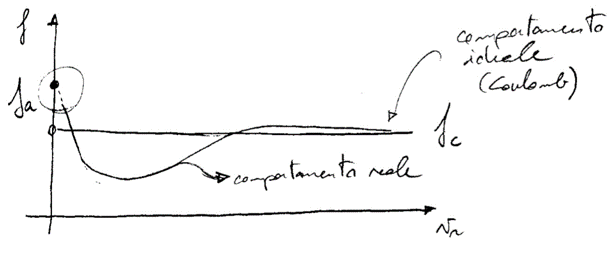
\includegraphics[width=.95\textwidth]{chapter05/Immagine164}
 \end{minipage}
 \hfill
 \begin{minipage}{.5\textwidth}
  Il coefficiente di attrito f definito come forza di attrito fratto la componente normale di reazione vincolare è una funzione della velocità di strisciamento che non si comporta esattamente come abbiamo modellato: il nostro modello prevede che fintanto che $v_r = 0$ il coefficiente $f = f_a$; nel momento in cui la velocità sia diversa da zero, tale coefficiente scatta istantaneamente $f = f_c$ che rimane costante per ogni valore della velocità di striasciamento.
\end{minipage}
\vspace{1mm}

 Nella realtà, invece, si ha che l'andamento di questo coefficiente f in funzione della velocità è inizialmente decrescente, può poi presentare una parte nuovamente crescente e avvicinarci al valore $f_c$, che noi associamo in maniera univoca alle condizioni cinetiche.

Il modello che abbiamo seguito fino ad ora per descrivere l'interazione di due corpi a contatto (ovvero con aderenza o strisciamento relativo) è il modello di Coulomb, che è un modello fenomenologico: non si preoccupa di descrivere il fenomeno dal punto di vista microscopico, ma si focalizza sulla descrizione delle componenti risultanti di forza, che però nascono da dei fenomeni microscopici talvolta molto complessi.

Il modello Coulombiano arriva alla definizione di un coefficiente di attrito cinetico definito come il rapporto tra la componente di reazione vincolare tangenziale ($T_c$) e la componente normale N. Alcune semplificazioni vengono proposte dal modello di Coulomb:
\begin{itemize}
\item  Il coefficiente d'attrito $f_c$ non dipende da:
\begin{enumerate}
\item Il carico normale N: il rapporto $f_c$ infatti è una costante;
\item La velocità relativa tra i corpi (velocità di strisciamento);
\item L'area apparente delle superfici a contatto;
\end{enumerate}
\item Il coefficiente d'attrito $f_c$ dipende da:
\begin{enumerate}
\item La natura dei materiali a contatti;
\item Lo stato delle superfici (rugosità, finitura superficiale, puliza e contaminazione);
\end{enumerate}
\end{itemize}

La ricerca in questo campo ha portato delle conclusioni un po' diverse dal modello Coulombiano che estendono e rendono più efficacie il modello di attrito. L'attrito infatti dipende da:
\begin{enumerate}
\item La natura e le caratteristiche delle superfici a contatto hanno una forte influenza sull'attrito
\item Lo stato delle superfici hanno una forte influenza sull'attrito
\item La temperatura
\item La pressione di contatto governata dall'area apparente (più che dall'area di contatto)
\item La velocità di strisciamento
\item Il tempo di contatto
\end{enumerate}
che il modello Coulombiano non considera.

Secondo un'interpretazione più moderna dei fenomeni di attrito la componente tangenziale, che giace nel piano del vinolo, è somma di alcuni contributi che nascono a livello microscopico: più in particolare la componente \textbf{T} può essere scritta come somma di 4 contributi principali.
\[T = T_1 + T_2 + T_3 + T_4\]
Vediamo brevemente il comportamento di ciascuno di questi contributo all'attrito totale che si verifica tra le due superfici.
\begin{enumerate}
\item $\mathbf{T_1}$ è il contributo legato alla rottura delle microgiunzioni.

Se riprendiamo il modello di contatto tra due superfici a livello microscopico sappiamo che il contatto avviene tra delle asperità che costituiscono una frazione piuttosto piccola dell'area apparente di contatto. In queste asperità a contatto reciproco nascono delle microgiunzioni: il materiale ricrea la continuità e quindi crea delle saldature che si oppongono al movimento relativo di un corpo rispetto all'altro.

Se proviamo a proporre un modello semplificato di questo fenomeno possiamo scrivere che la forza di attrito che nasce dall'esigenza di rompere le microgiunzioni ($T_1$) può essere espressa come la somma della resistenza a taglio delle microgiunzioni stesse.
\[T_{1,i} = \tau_s\,A_i\]
dove:
\begin{itemize}
\item $\tau_s$ è la sollecitazione a taglio che porta alla rottura della microgiunzione (Forza/superficie). Se pensiamo che il materiale sia uniforme sulla superficie di contatto la $\tau_s$ è comune a tutti gli i-esimi contributi e può essere raccolta nella sommatoria.
\item $A_i$ è la superficie i-esima che si realizza alla saldatura/giunzione tra due asperità
\end{itemize}
Il valore di sollecitazione complessivo:
\[T_1 = \sum_i\,T_{1,i} = \tau_s\,\sum_i\,A_i = \tau_s\,A_r\]
Sappiamo anche che l'area reale $A_r$ è calcolabile come la forza normale alla superficie fratto la durezza Brinell ($A_r = F / HB$), che risulta essere una discreta approssimazione dell'andamento dell'area reale.

Facendo tale espressione si trova che:
\[T_1 = \cfrac{\tau_s}{HB}\,F\]
Questa relazione, seppur in maniera approssimata ci propone la proporzionalità tra $T_1$ (ovvero lo sforzo per la rottura delle microgiunzioni) e F (ovvero la forza normale complessivamente sopportata dal contatto a strisciamento).

Si può calcolare, a questo punto, il coefficiente di attrito cinetico come:
\[f_c = \cfrac{T_1}{F} = \cfrac{\tau_s}{HB}\]
Per i metalli esistono delle relazioni approssimate che legano queste grandezze alla $\sigma_{ys}$: $\tau_s\,\approx 0.5 \sigma_{ys}$ e $HB \approx 3\,\sigma_{ys}$.
Questo porterebbe il valore atteso di $f_c$ ad essere pari a 1/6.

Si osserva sperimentalmente però che questo valore non è seguito nemmeno dai metalli da questo modello predittivo, in quanto ci sono alcune condizioni che il modello ha trascurato, ad esempio: al contatto tra due superfici si frappone una serie di contaminanti che sono quasi sempre presenti e dipendono quasi sempre dalla lavorazione o manipolazione delle superfici. 

Ci sono una serie di proprietà locali del materiale che sono differenti rispetto alle proprietà del metallo prese a riferimento per il calcolo. 

\begin{minipage}{.5\textwidth}
Quello che ci si attende è che all'aumentare del livello di contaminazione, l'area apparente di contatto rimane grosso modo la stessa, ma quello che cambia è la resistenza a taglio della giunzione ($\tau_s$).

Dal punto di vista sperimentale osserviamo infatti che il coefficiente $f_c$, è fortemente dipendente dalla contaminazione: al diminuire della contaminazione in generale aumenta $f_c$ sia per i materiali metallici che non; all'aumentare della contaminazione il comportamento dei materiali metallici e non metallici tende a convergere.
\end{minipage}
\hfill
\begin{minipage}{.5\textwidth}
\centering
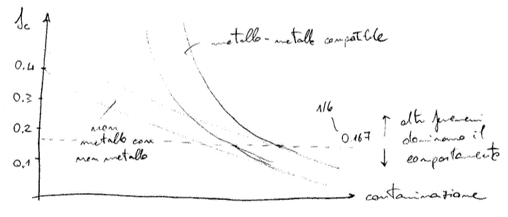
\includegraphics[width=.95\textwidth]{chapter05/Immagine165}
\end{minipage}

\item $\mathbf{T_2}$ è il contributo legato alla deformazione delle asperità.

Essa rappresenta la forza necessaria per provocare la deformazione anelastica delle asperità che localmente, singole coppie di asperità, si verifica: il materiale si distribuisce e nel fare ciò assorbe dell'energia.
\item $\mathbf{T_3}$ è il contributo legato al taglio e all'asportazione delle asperità. La differenza con $T_2$ è che in questo caso ci si riferisce a quelle asperità che a causa del moto relativo vengano tagliate e asportate: il meccanismo non è più solo una ridristibuzione locale del materiale, ma anche la creazione di nuova superficie a cui è associata una forma di energia che deve essere fornita al sistema.

Tale meccanismo inoltre può prevedere la formazione di corpi terzi rispetto ai due corpi nominalmente presenti al contatto strisciante.
\item $\mathbf{T_4}$ è il contributo legato al meccanismo di solcatura.

Esso è connesso alla deformazione elastica del materiale, ma in questo caso non più a livello microscopico, ma a livello macroscopico, con una scala di spostamenti che sia confrontabile con l'entità dello spostamento relativo tra le due superfici.
\end{enumerate}

\subsection{Principali fattori che influenzano l'attrito}
Senza andare nel dettaglio a livello microscopico ci sono delle conclusioni abbastanza generali che si possono trarre e descrivere anche solo con dei grafici
\begin{enumerate}
\item \textbf{Rugosità superficiale}:

Si verifica sperimentalmente che lo stato di finitura delle superfici ha una certa influenza sul coefficiente di attrito e, prendendo la rigosità come parametro che quantifica il livello di finitura superficiale, bassi valori di rugosità implicano superfici dalla finitura molto spinta mentre alte valori di rugosità indicano superfici molto grezze.

Quando la finitura è molto spinta si ossserva che il coefficiente di attrito cinetico tende ad aumentare e questo è dovuto al fatto che livelli di finitura alti portano ad aumentare l'area reale di contatto rispetto al valore ipotetico quantificato come il rapporto tra la forza normale alla superficie di contatto e la durezza Brinell ($A_r = F/HB$).

\begin{center}
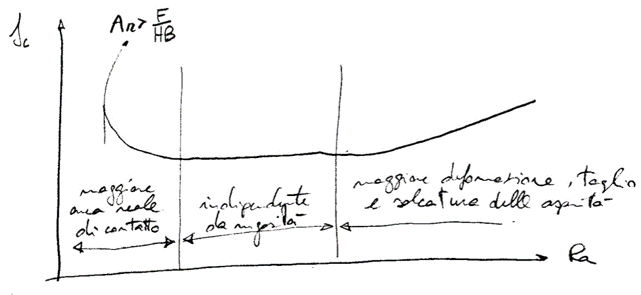
\includegraphics[width= .7\textwidth]{chapter05/Immagine166}
\end{center}

L'aumento dell'area reale di contatto promossa dal fatto che lo stato superficiale è molto rifinito porta ad aumentare il coefficiente di attrito rispetto a questo valore di riferimento.

È presente un range intermedio di rugosità per il quale il coefficiente di attrito cinetico è in grosso modo indipendente dalla rugosità: non sono presenti variazioni significative dei fenomeni che abbiamo elencato rispetto alla rugosità stessa.

Tuttavia, superata una certa soglia, la rugosità torna ad influire sul coefficiente di attrito: in particolare aumentando la rugosità ciò che si ottiene è che si ha un aumento del coefficiente di attrito. Si fanno infatti a potenziare quei fenomeni di deformazione delle asperità, taglio delle asperità e solcatura.

Tanto più grezza la superficie tanto più si ha che si creino interazioni di tipo anelastico tra la superficie e corpi esterni alla sola coppia di superfici nominali: questo porta ad un potenziamento dell'interazione tra le due superfici secondo questi meccanismi e un conseguente aumento del coefficiente di attrito cinetico.
\item \textbf{Velocità relativa}:

Sappiamo che nel modello semplificato, è presente un  coefficiente di attrito statico che vale per strisciamento nullo e un passaggio a coefficiente di attrito cinetico che vale per velocità diverse da zero.

Nella realtà tale transizione avviene in un intervallo di velocità molto ristretto dopodiché si ha un comportamento del coefficiente di attrito cinetico che è più complesso di quanto si evidenzia nel modello di Coulomb: in particolare si ha che per velocità di trasciamento molto piccole il coefficiente di attrito tende ad aumentare (si pensa che questo sia legato al fatto che le microgiunzioni presentano una resistenza crescente in questo range di velocità con la velocità stessa); si raggiunge un valore di massimo del coefficiente di attrito cinetico e un calo del coefficiente stesso che porta il suo valore a quello assunto come riferimento attorno a velocità di striasciamento del metro al secondo.

\begin{center}
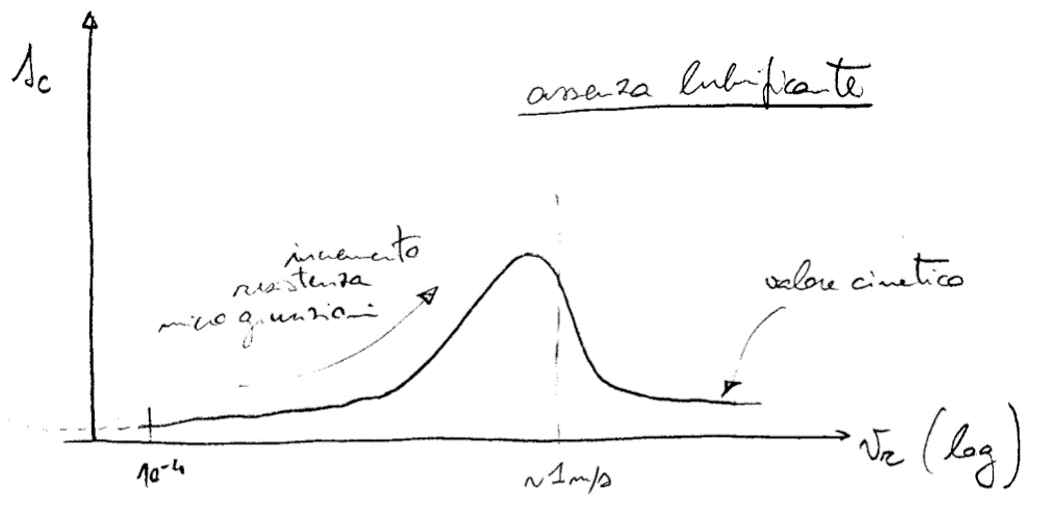
\includegraphics[width= .7\textwidth]{chapter05/Immagine167}
\end{center}

Si è quindi realizzata la transizione tra attrito statico e cinetico e da questo punto in poi è più corrispondente alla realtà il modello semplificato di Coulomb (in condizioni di assenza di lubrificante).

Se invece la coppia cinematica è lubrificata (inserimento di lubrificante al contatto tra i due corpi), si parla di lubrificazione idrodinamica: il lubrificante in questa condizione è interposto in maniera passiva tra i due corpi e viene trascinato in movimento, dove si crea una pressione al meato fluido che promuove la separazione delle due superfici limitando il contatto diretto.

\begin{center}
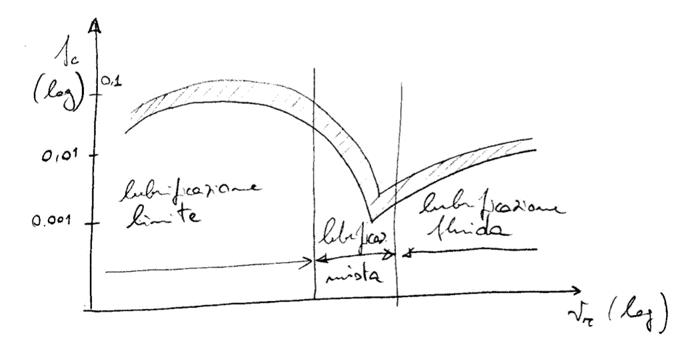
\includegraphics[width= .7\textwidth]{chapter05/Immagine168}
\end{center}

A seconda della velocità relativa tra i due corpi questa interposizione di lubrificante può essere piò o meno efficace: nel grafico proposto viene rappresentato l'andamento del coefficiente di attrito cinetico in funzione della velocità di strisciamento in presenza di lubrificante.

Con valori di velocità di strisciamento basse si parla di \textbf{lubrificazione limite}: basse velocità non permettono la creazione di uno strato di lubrificante che separi completamente i due corpi per cui non si riesce a evitare il contatto tra i due materiale. Questo porta il coefficiente di attrito ad assumere valori relativamente elevati.

Quando la velocità di strisciamento aumenta viene promosso l'aumento di pressione dello strato di lubrificante, il che comporta l'aumento della separazione dei due corpi. Si passa da una lubrificaizone limite ad una \textbf{lubrificazione mista}, in cui si riesce a separare i due corpi in una certa misura e il coefficiente di attrito diminuisce raggiungendo il suo valore minimo.

Aumentando ulteriormente la velocità, la pressione del fluido è sufficiente a mantenere la separazione tra le due superfici, però cominciano a entrare in gioco fenomeni di dissipazione all'interno del fluido: si osserva che il coefficiente di attrito in regime di \textbf{lubrificazione fluida}, tende ad aumentare non più per le caratteristiche di interazione tra i materiali, ma per le caratteristiche di viscosità del fluido lubrificante.

L'andamento decrescente del coefficiente di attrito provoca un comportamento dinamico dello \textbf{stick-slip}: il moto avviene per continuo passaggio dalla situazione di aderenza a quella di strisciamento; questo comportamento è caratteristico delle basse velocità di strisciamento. All'aumentare della velocità si entra in una regione in cui il coefficiente di attrito non è più decrescente, ma è crescente rispetto alla velocità e questo porta alla cancellazione di questo fenomeno tipico delle coppie cinematiche e degli accoppiamenti freno-pastiglia.

\item \textbf{Tempo di contatto (in assenza di movimento)}

Consiste nel tempo di assenza di movimento alla coppia cinematica. Supponiamo di avere un sistema composto da due corpi tra i quali è presente dell'attrito, e che sia mantenuto a velocità costante il movimento di un corpo rispetto all'altro. Sappiamo che in questa condizione la forza necessaria ad applicare è pari al coefficiente di attrito cinetico per la componente di normale (e quindi una forza tangenziale nota e costante).

Supponiamo a questo punto di arrestare il sistema e mantenersi in quiete per un certo intervallo di tempo: la forza tangenziale inizialmente diminuisce, si porta a zero quando il sistema raggiunge la quiete, per far ripartire il sistema (se l'intervallo di tempo/d'arresto è piuttosto basso) è sufficiente far risalire il valore di forza tangenziale al valore che manteneva il sistema in movimento in condizioni cinetiche.

Non è necessario quindi raggiungere il valore del coefficiente di aderenza per la componente normale di forza, ma è sufficente raggiungere il valore del coefficiente di attrito cinetico per la componente normale di forza.

Supponiamo di ripetere l'esprienza fermandoci per valori dell'intervallo di tempo maggiori: per far ripartire il sistema, sarà necessario far aumentare la forza T tangenziale, fino ad un valore che non sarà più $T = f_c\,N$, ma superiore. Sarà, di conseguenza, necessario che il rapporto T/N raggiunga un valore $f_{\overset{\_}{a}}$ leggermete superiore a $f_c$ che caratterizzava il moto del sistema in condizioni stazionarie.

Maggiore è il tempo di arresto più il valore di soglia da varcare per riportae il sistema in movimento aumenta.

Il coefficiente di aderenza può essere interpretato come il limite di $f_{\overset{\_}{a}}$ per un tempo di arresto infinitamente lungo: in un diagramma di $f_{\overset{\_}{a}}$ con il tempo osserviamo che tale coefficiente ha un valore crescente che tende asintoticamente al valore del coefficiente di aderenza.

\begin{center}
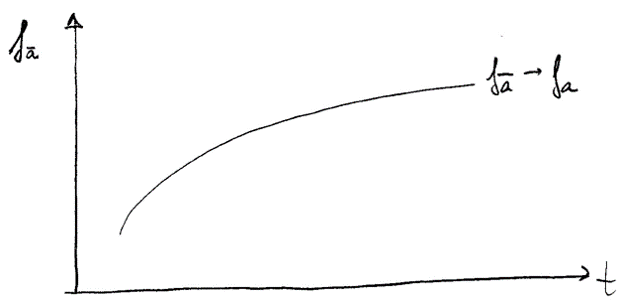
\includegraphics[width= .7\textwidth]{chapter05/Immagine169}
\end{center}

Si ritiene che questo sia causato dal fatto che una volta che il sistema si arresta le microgiunzioni non si creano immediatamente, ma è un processo che richiede del tempo; quando il tempo di arresto è inferiore al tempo caratteristico che governa la formazione di queste giunzioni la fermata non ha avuto nessuna influenza sulla situazione di contatto a livello microscopico e il sistema può ripartire senza l'esigenza di rompere microgiunzioni aggiuntive che si sono formate in più rispetto alla normale condizione cinetica. 

Se invece il tempo di permanenza in quiete è sufficientemente più grande del tempo caratteristico di formazione delle microgiunzioni il sistema ha cambiato stato e ha raggiunto le condizioni di aderenza. Tra questi due casi limite sono presenti tempi di arresto intermedi che portano la condizione di funzionamento in regime intermedio.

\item \textbf{Pressione di contatto e area apparente di contatto}:

Sappiamo che l'area apparente di contatto è poco significativa e ciò che effettivamente conta per il meccanismo di creazione e rottura delle microgiunzioni è l'area reale. Il modello che avevamo trovato ci suggeriva che l'area reale fosse proporzionale alla forza normale alla superficie di contatto (dove il fattore di proporzionalità era l'inverso della durezza Brinell) e questo rapporto moltiplicato per la $\tau$ di rottura delle micro-giunzioni descriveva bene la proporzionalità della forza d'attrito nei confronti della forza normale.

Questo modello, tuttavia, ha dei limiti e si riscontra che quando le superfici sono particolarmente liscie il coefficiente di attrito sembra dipendere dall'area apparente e quindi anche la forza d'attrito dipenderà da essa secondo una relazione crescente dell'area apparente di contatto.

Una questione analoga si rileva anche per la pressione: si osserva che nelle operazioni di laminazione il coefficiente di attrito risulta sensibile alla pressione di contatto nonostante il modello di Coulomb non prevede dipendenza da area e pressione, ma solo dalla forza normale di contatto.

\item \textbf{Temperatura}

Si osserva che la temperatura ambientale ha una certa influenza sul coefficiente di attrito: da un lato questo avviene perché la temperatura influenza le prorpietà meccaniche dei materiali ed è quindi normale che l'attrito ne venga influenzato di conseguenza (cfr. localmente la temperatura può arrivare a valori elevati portando alla riduzione della $\tau_s$ più di quanto aumenta l'area reale di contatto, con conseguente riduzione del coefficiente di attrito).

Diverse categorie di materiali si comportano in maniera diversa: nel grafico riportato (T, $f_c$) i materiali sintetici, in generale, hanno un andamento non univoco (ci possono essere dei regimi di temperatura in cui il coefficiente di attrito cinetico è pressoché costante ad altri intervalli di temperatura in cui tale coefficiente è decrescente).

\begin{center}
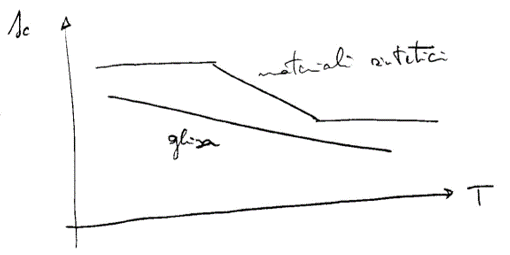
\includegraphics[width= .7\textwidth]{chapter05/Immagine170}
\end{center}

Un caso particolare è quello della ghisa (materiale spesso utilizzato per fare i dischi freno): il comportamento della ghisa è caratterizzato da un calo del coefficiente di attrito cinetico rispetto alla temperatura; tanto più il materiale è caldo tanto più è basso l'attrito che riesce a provocare.

Se si pensa alla sua applicazione nei freni a disco, questa caratteristica risulta essere un limite tecnologico del sistema perché il surriscaldamento dei freni comporta una perdita di efficienza direttamente legata al calo del coefficiente di attrito cinetico.
\end{enumerate}

\subsection{Usura}

L'\textbf{usura} è un fenomeno di perdita di materiale da parte delle superfici che si trovano in moto relativo uno con l'altro e che è necessario tenere conto per	eseguire la manutenzione della coppia cinematica e prevederne la durata o anche per poterla progettare in maniera corretta.

Ci sono diversi meccanismi che promuovono l'usura al contatto tra superfici striscianti:
\begin{itemize}
\item \textbf{Usura adesiva}: al contatto tra due superfici si creano delle microgiunzioni e quindi delle microsaldature che tendono a ricreare la continuità del materiale tra i due corpi. Mantenendo in movimento con una certa forza T le due superfici si crea una continua rottura e riformazione di queste microgiunzione, in particolare alla rottura di esse si possono creare delle \textbf{particelle di usura}, ovvero dei corpi microscopici si staccano dalle superfici che possono essere reintegrati in una delle due superfici oppure eliminati dal lubrificante.

È tuttavia importante tenere a mente che le dimensioni caratteristiche delle particelle di usura dipendono dalle proprietà del materiale; tendenzialmente quando il materiale è molto duro (come un ossido) le dimensioni possono essere dell'ordine del micron, quando invece il materiale delle superfici è un metallo tenero (come il piombo) le dimensioni di queste particelle possono raggiungere anche il centinaio di micron.

Quando si progetta la coppia cinematica è fondamentale tenerne conto in quanto è opportuno dimensionare in maniera opportuna la lubrificazione di queste superfici, ma anche dimensionare l'accoppiamento / gioco che si lascia tra le superfici. Lasciare giochi troppo ristretti quando le particelle di usura sono troppo grandi può addirittura essere controproducente.
\item \textbf{Usura abrasiva}: usura causata dalla presenza di particelle di caratterisiche diverse da quelle dei substrati in particolare si tratta di particelle più dure che possono essere sia endogene (ovvero intrinseche ai due corpi in moto relativo) o esogene (ovvero particelle terze rispetto alle due superfici a contatto).

Particelle dure possono essere ad esempio inclusioni di ossidi oppure anche materiale del substrato con caratteristiche meccaniche alterate dall'incrudimento oppure differenze sostanziose tra la durezza dei due materiali.

Questi due processi di usura a 2 o 3 corpi comunque si basano sulla presenza di caratteristiche del materiale coinvolto nel meccanismo particolarmente alterate e efficaci nel promuovere l'esportazione di materiale.

\item \textbf{Usura erosiva o erosione}: legato al fatto che particelle estranee alle due superfici possono provocare l'esportazione di materiale in virtù della loro stessa velocità di impatto e quindi di erodere le due superfici per impatto con le superfici stesse
\item \textbf{Usura corrosiva}: legata alla degradazione delle superfici per azione meccanica e chimica combinate. Il tipico esempio è quello che l'azione meccanica tende a rimuovere gli ossidi che normalmente tenderebbero a proteggere le superfici dall'usura (avendo caratteristiche meccaniche particolarmente elevate), l'azione protettiva viene a mancare quando l'ossido è rimosso e il materiale sottostante si ritrova esposto al meccanismo di usura.
\item \textbf{Usura per fatica}: esistono spesso all'interno dei metalli dei danneggiamenti/cricche/cavità che tendono a propagarsi se sottoposti a carichi alterni. La propagazione di queste imperfezioni può arrivare a produrre un distacco di materiale per sfogliatura.

Questi danneggiamenti sono spesso promossi da inclusioni, precipitati e qualunque alterazione della continuità del materiale metallico. Anche questo meccanismo combinato con gli altri può promuovere la perdita del materiale da parte delle superfici.
\end{itemize}

C'è un'ipotesi che permette di fare un calcolo approssimato del volume complessivo delle particelle di usura generate a un certo accoppiamento strisciante: l'\textbf{Ipotesi di Raye}.

Essa consiste in un'ipotesi molto semplificativa che si trova a descrivere in maniera sufficientemente accurata per calcoli preliminari condizioni di usura dominate da fenomeni adesivi e abrasivi.

Se ci interessa avere una descrizione approssimata del volume complessivo delle particelle di usura quando ci siano fenomeni adesivi e abrasivi rilevanti al contatto, si esegue un calcolo del seguente tipo:

Sappaimo che il rapporto tra la forza normale (con cui forziamo il corpo in movimento sul corpo fisso) e la durezza Brinell è l'area reale di contatto. 

Supponiamo che una frazione dell'area reale di contatto sia quella che associamo alla creazione di particelle di usura (ovvero non tutte le microgiunzioni generano particelle di usura, ma è un evento che si verifica con una certa probabilità statistica) e se pensiamo di portare in movimento un corpo rispetto all'altro questo fenomeno andrà a generarsi con una certa frequenza man mano che procede lo strisciamento.

In particolare, al fine di quantificare tale proprietà globalmente tramite un coefficiente K, si può enunciare l'espressione:
\[V = K\,\cfrac{F}{HB}\,l\]
dove:

\begin{minipage}{.55\textwidth}
\begin{itemize}
\item $K\,\cfrac{F}{HB}$ è il volume totale delle particelle di usura generate per unità di lunghezza di strisciamento, sempre se le condizioni di strisciamento rimangono sempre le stesse.
\item V e il volume totale delle particelle di usura
\item l è la distanza percorsa
\end{itemize}
\end{minipage}
\hfill
\begin{minipage}{.4\textwidth}
\centering
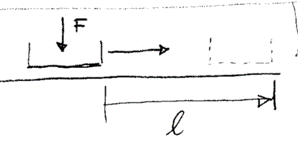
\includegraphics[width=.95\textwidth]{chapter05/Immagine171}
\end{minipage}

Questa relazione semplificata chiama in causa un certo modello probabilistico di formazione di particelle di usura come una frazione dell'area reale di contatto e quindi della forza normale che si esercita.

Osserviamo che di fatto il volume è proporzionale al prodotto $F\cdot l$. Pensando che in condizioni di strisciamento la forza tangenziale è una frazione della forza normale (quindi la forza F è proporzionale a T, che è la forza d'attrito) il prodotto $F\,\cdot \,l$ sarà proporzionale a $T\,\cdot\,l$. 

Questa espressione, in cui al posto di usare F utilizziamo T è utile in quanto evidenzia che il volume complessivo delle particelle d'usura è proporzionale al lavoro di attrito

Possiamo riformulare l'ipotesi di Reye scrivendo che il volume complessivo delle particelle di usura è proporzionale mediante una nuova costante (K') al lavoro di attrito:
\[V = K^{,}\,T\,l\]
Questo punto di vista sull'usura è di tipo energetico in quanto mette in relazione un lavoro fatto dalle forze d'attrito con un volume messo in relazione alla formazione di nuova superficie.

La creazione di nuova superficie infatti richiede energia, che in questo caso è fornita dall'attrito.
	
	\begin{center}
	{\scshape {\bfseries Esempio applicativo:}}
	\end{center}
Una possibile applicazione dell'ipotesi di Reye è quella del calcolo dell'andamento delle pressioni al contatto strisciante tra un albero che ruota e un supporto fisso. 

Supponiamo di avere un albero ad asse verticale che poggia su un supporto a strisciamento: ci può interessare calcolare l'andamento delle pressioni al contatto tra i due corpi.

\begin{minipage}{.65\textwidth}
Possiamo partire dall'ipotesi di Reye per cui il volume complessivo delle particelle di usura è proporzionale al lavoro delle forze d'attrito secondo una costante di proporzionalità (K').

Dall'analisi della figura proposta possiamo immaginare di isolare un volume infinitesimo di materiale sull'albero (che è in rotazione con la velocità angolare $\omega$) pensando che tale volume sia una corona circolare estrusa in direzione assiale.

Tale corona circolare presenta un raggio (r), uno spessore infinitesimo (dr) e un'altezza ($\delta$) che corrisponde all'effetto di usura in un intervallo di tempo $\Delta t$.
\end{minipage}
\hfill
\begin{minipage}{.3\textwidth}
\centering
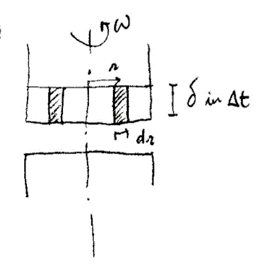
\includegraphics[width=.8\textwidth]{chapter05/Immagine172}
\end{minipage}

Possiamo quindi riscrivere l'equazione dell'ipotesi di Reye in termini differenziali secondo la seguente equazione:
\[dV = K^{`}\,dL\]
dove dL è il lavoro fatto dalle forze di attrito che agiscono sulla superficie dell'anello preso in esame.

Possiamo esprimere questo volume dal punto di vista geometrico come il prodotto della superficie circolare per l'altezza assiale di cui estrudiamo idealmente la corona circolare ($\delta$):
\[dV = \delta \cdot 2\,\pi\,r\,dr\]

\begin{minipage}{.5\textwidth}
Proviamo a calcolare il lavoro delle forze d'attrito.

Calcoliamo innanzitutto il momento esercitato dalle forze di attrito che sono applicate alla corona circolare infinitesima: tale momento può essere calcolato come:
\[dM = r\,\int dT\]
dove dT è la forza d'attrito che agisce sull'elemento infinitesimo della corona circolare, che può essere espresso come il prodotto del coefficiente di attrito cinetico ($f_c$) per la componente normale di forza (dN)
\end{minipage}
\hfill
\begin{minipage}{.5\textwidth}
\centering
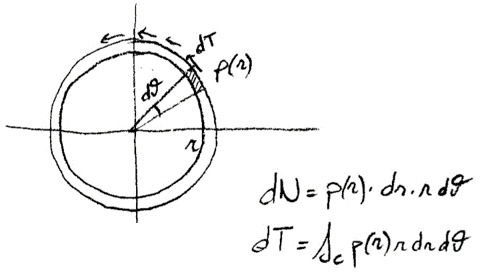
\includegraphics[width=.8\textwidth]{chapter05/Immagine173}
\end{minipage}

\[dN = p(r)\,dr\,r\,d\theta \qquad;\qquad dT = f_c\,dN = f_c\,p(r)\,dr\,r\,d\theta\]
dove p(r) è l'andamento delle pressioni lungo la corona circolare. Sostutuendo all'integrale del momento:
\[dM = r\,\int_{0}^{2\,\pi}\,f_c\,p(r)\,r\,dr\,d\theta\,=\,2\,\pi f_c\,p(r)\,r^2\,dr\]
Il lavoro di questo momento si puo semplicemente calcolare come:
\[dL = dM\,\omega\,\Delta t = \omega\,\Delta t \,2\,\pi\,p(r)\,r^2\,dr\]
dove $\omega\,\Delta t$ è la rotazione relativa dell'albero rispetto al supporto

Eguagliando a questo punto le due espressioni si ottiene:
\begin{align*}
dV &= K'\,dL\\
\delta \cdot \cancel{2\,\pi\,r\,dr} &= K'\, \omega\,\Delta t \,\cancel{2\,\pi}\,p(r)\,r^{\cancel{2}}\,\cancel{dr}\\
p(r) &= \cfrac{\delta/\Delta t}{K'\,f_c\,\omega}\cdot\cfrac{1}{r} = \cfrac{K''}{r}
\end{align*}

dove:
\begin{itemize}
\item $\delta / \Delta t$ è la velocità di usura in quanto è il rapporto tra l'altezza usurata e il tempo in cui tale usura si verifica 
\item $K'\,f_c\,\omega$ è una costante
\end{itemize}

Abbiamo dunque ottenuto che l'andamento della pressione tra le due superfici è inversamente proporzionale al raggio: quando siamo in prossimità dell'asse di rotazione dell'albero le pressioni raggiungono valori teoricamente infiniti e questo ci deve suggerire come progettare correttamente il cuscinetto.

Infatti possiamo progettare il cuscinetto evitando di mettere materiale d'usura in prossimità dell'asse altrimenti lavorerebbe a pressioni sicuramente superiori alla pressione tollerabile dal materiale in quel punto.

Possiamo inoltre trovare la costante K'' eguagliando l'integrale delle pressioni alla forza assiale complessiva che deve essere sostenuta dal cuscinetto:
\begin{align*}
\int_{r1}^{r2}\,p(r)\,2\,\pi\,r\,dr &= F\\
\int_{r1}^{r2}\,\cfrac{K''}{\cancel{r}}\,2\,\pi\,\cancel{r}\,dr &= F\\
2\,\pi\,(r_2 - r_1)\,K'' &=F\\
K'' &= \cfrac{F}{2\,\pi\,(r_2\,-\,r_1)}
\end{align*}

Sostituendo tale costante di proporzionalità nella legge che dettava l'andamento delle pressioni:
\[p(r) = \cfrac{F}{2\,\pi\,r\,(r_2\,-\,r_1)}\]
Secondo tale andamento si può osservare che in realtà sotto un certo valore di $r_1$ al di sotto del quale non è opportuno che ci sia contatto in quanto le pressioni sarebbero superiori alla resistenza del materiale.

\section{Lezione 22-04 -- Daniele Bortoluzzi}

\subsection{Attrito di rotolamento}

Anche al rotolamento di un corpo volvente sulla superficie nascono delle azioni che sostanzialmente si oppongono al rotolamento del corpo sulla superficie. Questo fenomeno è descritto dall'attrito di rotolamento o attrito volvente che è un fenomeno comunque rilevante dal momento che molto spesso si realizza, dal punto di vista tecnologico, il puro rotolamento dei corpi rispetto a superfici.

\begin{minipage}{.65\textwidth}
Prendiamo il caso indicato in figura in cui si ha un corpo volvente (cilindro) posto in puro rotolamento su una superficie. Il corpo volvente rotola con una velocità angolare $\omega$ ed è forzato contro la superficie tramite una componente normale N.
	
Quello che succede è che al contatto, che nominalmente è un punto fermo, si ha una condizione di staticità (non si ha strisciamento) e la reazione vincolare è una forza F, generalmente indeterminata all'interno del cono di attrito statico.

Oltre a questo nascono sulla superficie di contatto delle azioni che risultano in due componenti di momento: 
\end{minipage}
\hfill
\begin{minipage}{.35\textwidth}
\centering
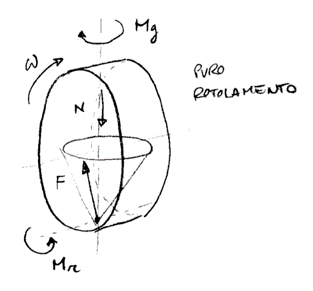
\includegraphics[width=.95\textwidth]{chapter05/Immagine174}
\end{minipage}

\begin{itemize}
\item La coppia di attrito di rotolamento ($\mathbf{M_r}$) che si oppone al rotolamento stesso
\item La coppia di attrito di giro ($\mathbf{M_g}$) che è un momento ad asse verticale
\end{itemize}

Mentre la prima componente si oppone al rotolamento, la seconda è una componente che promuoverebbe, se non bilanciata, un \textbf{moto di prillamento}, ovvero rotazione del corpo volvente attorno ad un asse verticale.

L'azione combinata delle due componenti di momento è detto \textbf{Momento di attrito volvente} (M).

In condizioni statiche, le azioni che nascono al contatto tra i due corpi possono equilibrare dei momenti che applichiamo al corpo per farlo rotolare: applicando una coppia esterna che tenda a far rotolare il corpo sulla superficie, finché tale coppia non varca una certa soglia, il corpo volvente rimane fermo.

Esiste una relazione che esprime tale coppia limite come proporzionale alla forza con cui il corpo volvente è forzato contro la superficie (N): vale dunque la disuguaglianza
\[\norma{M_r} \le u_r\,\norma{N}\]
dove $u_r$ è detto parametro di attrito di rotolamento ed è dimensionalmente una lunghezza

Allo stesso modo possiamo dire che prima che inizi il moto vale anche che la coppia di attrito di giro è inferiore ad una certa soglia, la quale è sempre proporzionale alla forza N con cui forziamo il corpo volvente contro la superficie
\[\norma{M_g} \le\,u_g\,\norma{N}\]
dove $u_g$ è detto parametro di attrito di giro ed è dimensionalmente una lunghezza.

Quando esiste rotolamento tra corpo volvente e superficie sia la coppia di attrito di rotolamento che la coppia di attrito di giro risultano uguali ai valori di soglia. In queste condizioni definiamo i fattori di attrito volvente, riscalando i valori dei parametri di attrito di rotolamento e di giro rispetto alla dimensione caratteristica del corpo volvente (ad esempio il raggio):
\[
\begin{dcases}
f_v = \cfrac{u_r}{R}\\
f_{vp} = \cfrac{u_g}{R}
\end{dcases}
\]

\subsection{Resistenza al rotolamento (attrito volvente)}

\begin{minipage}{.65\textwidth}
Vediamo in questo schema un avista laterale del corpo volvente e della superficie sulla quale questo rotola.\newline

 La coppia di attrito di rotolamento ha una componente ortogonale al foglio e si oppone alla velocità angolare $\omega$.

Le azioni che sono applicate al corpo volvente sono:
\end{minipage}
\hfill
\begin{minipage}{.35\textwidth}
\centering
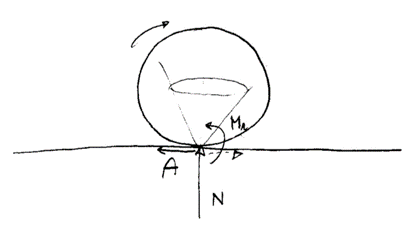
\includegraphics[width=.95\textwidth]{chapter05/Immagine175}
\end{minipage}

\begin{itemize}
\item l'azione normale N che è la componente normale alla reazione vincolare che si oppone alla forza con cui schiacciamo il corpo volvente contro la superficie;
\item la componente di attrito tangenziale A
\end{itemize}

L'insieme delle interazioni che avvengono sulla superficie di contatto causa una coppia $M_r$ che si oppone al rotolamento: in realtà vedremo che tale coppia nasce per una certa disuniformità di distribuzione delle pressioni sulla superficie di contatto (la quale non è puntiforma, ma ha una certa estenzione).

Avendo precedentemente scritto che la coppia di attrito di rotolamento è esprimibile come un parametro $u_r$ che moltiplica la componente normale N, stiamo già esprimendo in maniera implicita il fatto che la forza N nell'essere equilibrata dalle forze di contatto genera anche un certo braccio $u_r$.

Tale parametro è dunque una lunghezza, che difatti è chiamato anche parametro o braccio di attrito ed è espressa come un rapporto
\[u_r = f_v\,R\]
dove: $f_v$ è il fattore di attrito volvente e R è la dimensione caratteristica del corpo volvente.

Questo modello, per quanto semplificato, nasce dalla meccanica del contatto tra i due corpi anche nell'ipotesi che siano corpi a comportamento elastico lineare.

\begin{center}
{\scshape{\bfseries Rotolamento di corpi lisci su superfici lisce}}
\end{center}

Prendiamo il caso in cui ci occupiamo solamente della distribuzione delle pressioni al contatto tra i due corpi. Osserviamo che secondo la teoria di Hertz, se noi forzassimo un cilindro contro una superficie piana nell'ipotesi di elasticità lineare di comportamento del materiale, si ha un andamento delle pressioni parabolico, in cui la risultante, per l'equilibrio del sistema, passa per il centro del corpo.
\begin{center}
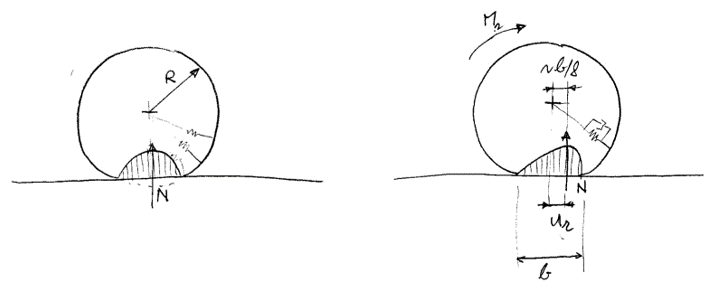
\includegraphics[width = .7\textwidth]{chapter05/Immagine176}
\end{center}

C'è un'impronta macroscopica la cui dimensione dipende dalla forza con cui forziamo il corpo contro la superficie (N).

Se supponiamo di porre in rotolamento il corpo volvente osserviamo che, nell'ipotesi che il materiale non abbia più solamente comportamento elastico, ma ci siano anche fenomeni dissipativi, nasce una certa dissimetria.

Proviamo a dare un'interpretazione di ciò che succede: se pensiamo che radialmente il nostro corpo si comporti come una molla, esse quando entrano nella superficie di contatto vengono compresse dal momento che la sua estremità non si muove più su una circonferenza, ma su un segmento, e essendo compresse acquisiscono energia in forma elastica potenziale.

A partire dal momento in cui l'estremità di queste molle arriva sull'asse di simmetria del corpo, quelle stesse molle tendono a rilassarsi restituendo l'energia elastica che hanno accumulato.

In un caso in cui si hanno solo fenomeni che possono accumulare energia e accumularne nella stessa quantità (fenomeni conservativi), non c'è motivo di avere dissimetria tra il comportamento in fase di compressione e quella di estensione della molla.

Se invece in parallelo a queste molle poniamo anche degli smorzatori (a indicare qualsiasi fenomeno dissipativo all'interno del materiale), ciò che succede è che nella fase di compressione la forza che la superficie piana deve esercitare sulla periferia del corpo volvente per comprimere il gruppo molla-smorzatore dovrà equilibrare sia la forza richiesta dalla molla che quella richiesta dallo smorzatore.

Nel momento in cui l'infinitesimo gruppo molla-smorzatore passa la mezzeria del corpo volvente dovrà estendersi per garantire il contatto della periferia del corpo volvente con la superficie piana. A tal fine la molla dovrà fornire la forza sia per estendere il gruppo, sia per garantire il contatto della periferia del corpo volvente con la superficie piana.

La forza utile che rimane per il contatto gruppo molla-smorzatore e la superficie piana è la forza che la molla esercita sottraendole la forza che richiede il gruppo morzatore per essere esteso: la forza netta che rimane tra la periferia del corpo volvente e la superficie piana sarà minore della quantità richiesta dall'elemento infinitesimo smorzatore (che dovrà essere esteso a spese dell'energia elastica accumulata dal corpo volvente).

Il risultato è che le pressioni al contatto tra corpo volvente e superficie piana non sono simmetriche rispetto all'asse di simmetria del corpo, ma: in fase di compressione saranno pressioni superiori a quelle che rimangono in fase di estensione.

L'andamento delle pressioni non è più simmetrico, ma prevede un andamento distorto in cui le pressioni sono maggiori nella metà dell'impronta che corrisponde alla compressione del corpo volvente, mentre saranno inferiori nella metà dell'impronta che corrisponde all'estensione del corpo volvente.

Il risultato è che l'andamento delle pressioni genera un risultante che deve comunque essere pari alla forza esterna applicata al corpo volvente in direzione verticale, ma non più localizzata nell'asse di simmetria del corpo stesso, ma spostata in avanti (nella direzione di avanzamento del corpo volvente) di una quantità $u_r$.

Osserviamo che per mantenere in movimento il corpo volvente è necessario applicare all'esterno una coppia uguale e contraria a questa $M_r = N\,u_r$.

Il parametro $u_r$ è un parametro che dipende dalle proprietà microscopiche del contatto tra il corpo volvente e la superficie: detta \emph{b} la dimensione dell'impronta, $u_r$ risulta una certa frazione di b. In generale per corpi metallici, l'ordine di grandezza di $u_r = b/8$.

Ricordiamo a questo punto che:
\[M_r = u_r\,N = R\,f_v\,N\]
Se utillizziamo la teoria di Hertz per il contatto elastico tra corpi osserviamo che nel caso di contatto cilindro piano la dimensione caratteristica dell'impronta, può essere calcolata come:
\[b = 1.52\,\sqrt{\cfrac{N}{E\,\rho\,l}}\]
dove:
\begin{itemize}
\item N è la forza normale
\item E è il modulo elastico del materiale
\item $\rho$ è il raggio equivalente al contatto tra i due corpi

In generale tra due corpi con raggio di curvatura $R_1$ (cilindro di raggio R) e $R_2$ (superficie piana di raggio di curvatura teoricamente infinito)
\[\rho = \cfrac{1}{R_1}\,+\,\cfrac{1}{R_2} = \cfrac{1}{R}\,+\,\cancel{\cfrac{1}{\infty}}\]
\item l è la profondità del cilindro
\end{itemize}

possiamo a questo punto calcolare
\[f_v = \cfrac{u_r}{R} \approx \cfrac{b/8}{R} \approx 0.2\,\sqrt{\cfrac{N}{E\,R\,l}}\]
In generale questo coefficiente varia con la velocità di rotolamento del corpo e il suo andamento è, qualitativamente, simile al coefficiente di attrito che passa da statico a cinetico e quindi risente della velocità relativa tra corpo.

In questo caso il rotolamento incipiente richiede un coefficiente $f_v$ leggermente più alto di quello dinamico.

\begin{center}
{\scshape{\bfseries Rotolamento di corpi lisci su superfici rugose}}
\end{center}

Di fatto il rotolamento su una superficie che presenta asperità implica la presenza di urti e quindi interazioni impulsive tra il corpo e le asperità stesse. Il comportamento a questo livello è piuttosto complesso in quanto dipende da come è distribuita l'irregolarità superficiale della pista sul quale rotola il corpo volvente, tuttavia anche in questo caso è possibile utilizzare un modello approssimato:
\begin{center}
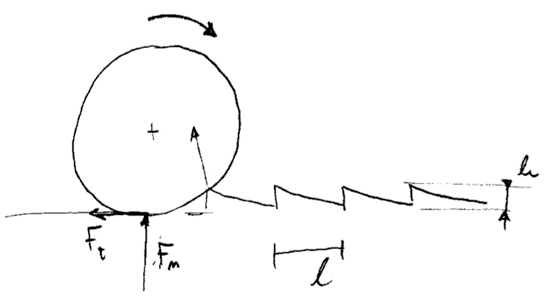
\includegraphics[width = .5\textwidth]{chapter05/Immagine177}
\end{center}

Consideriamo un corpo volvente sottoposto ad un certo carico normale, sappiamo che al contatto nascono due componenti (normale e tangenziale) e in questo modello nasce anche un'interazione al punto di contatto tra il corpo volvente e le asperità.

Consideriamo un'asperità caratterizzata da un'unica spaziatura \emph{l} tra le creste e una certa altezza \emph{h}: è possibile scrivere un modello in cui si arriva a calcolare che il coefficiente di attrito volvente ($f_v$) ha un andamento descritto dalla legge
\[f_v = c_1\,v^2\,+\,c_0\]
dove:
\begin{itemize}
\item La costante $c_1$ risulta proporzionale al rapporto tra l'altezza delle asperità e il prodotto \emph{R l} (R raggio del corpo volvente)
\[c_1 \propto \cfrac{h}{R\,l}\]
Nei casi più comuni di applicazione ingegneristica ha valore compreso tra i $6:8\,\cdot\,10^{-6}$.
\item La costante $c_0$ ha un ordine di grandezza di $1:2\,\cdot\,10^{-2}$
\end{itemize}

\begin{center}
{\scshape{\bfseries Esercizio n.1: aderenza e strisciamento}}
\end{center}

\begin{minipage}{.35\textwidth}
\centering
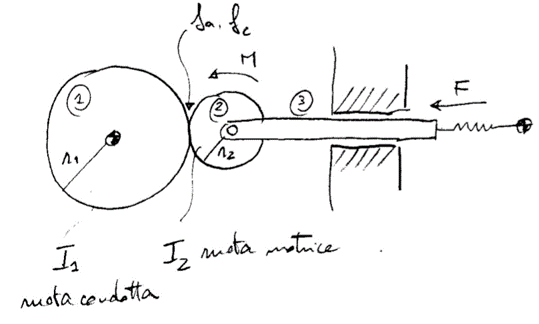
\includegraphics[width=.95\textwidth]{chapter05/Immagine178}
\end{minipage}
\hfill
\begin{minipage}{.65\textwidth}
Proponiamo un sistema che presenta un accoppiamento tra due ruote di frizione sul quale possiamo applicare i concetti che sono stati affrontati precedentemente.

Il sistema è descritto da due ruote di frizione (una ruota motrice e una ruota condotta) che vengono mantenute a contatto da una molla precaricata, mediante un'asta che scorre senza attrito su una guida. Il momento motore applicato alla ruota motrice mantiene in movimento il sistema secondo una legge del moto ignota a priori.
\end{minipage}

Ci viene richiedo di:
\begin{enumerate}
\item Trovare l'accelerazione angolare massima al corpo 1 (ovvero alla ruota condotta) affinché non ci sia strisciamento e il corrispondente momento applicato alla ruota motrice;
\item Illustrare cosa succede se il momento motore è maggiore di quello massimo per evitare lo strisciamento
\end{enumerate}

È necessario scrivere le equazioni del moto del sistema: per fare ciò lo disassembliamo evidenziando i momenti e le forze che agiscono su ciascun corpo rigido. Lo schema è proposto di seguito.
\begin{center}
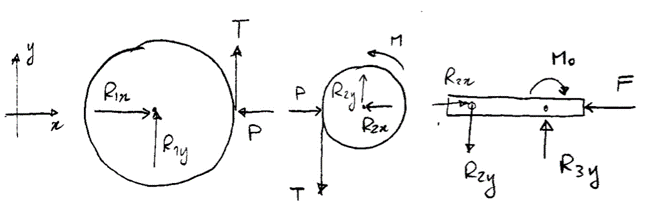
\includegraphics[width=.7\textwidth]{chapter05/Immagine179}
\end{center}

Procediamo alla scrittura delle equazioni del moto del sistema:

Selezioniamo le equazioni che sono realmente di interesse per la soluzione del problema, quindi:
\begin{enumerate}
\item \textbf{Equilibrio alla rotazione delle due ruote}. Ricordiamo che T è la componente tangenziale di reazione vincolare di attrito che ha una certa relazione con la componente normale P sulla base delle condizioni effettive (esse siano di aderenza o strisciamento).
\begin{itemize}
\item Rotazione corpo 1: (il centro di massa del corpo e il punto fisso coincidono)
\[I_1\,\ddot{\theta_1} = r_1\,T\]
\item Rotazione corpo 2: (verranno trascurate le due componenti di reazione vincolare in quanto non hanno braccio rispetto al centro)
\[I_2\,\ddot{\theta_2} = r_2\,T\,+\,M\]
\end{itemize}
\item \textbf{Equilibrio alla traslazione}
\begin{itemize}
\item Traslazione lungo l'asse x del corpo 2:
\[m_2\,\ddot{x_2} = P\,-\,R_{2x}\]
Imponendo che $\ddot{x_2} = 0$ in quanto la ruota motrice non ha movimento orizzontale, possiamo esprimere 
\[P = R_{2x}\]
\item Traslazione lungo l'asse x del corpo 3:
\[m_3\,\ddot{x_3} = R_{2x}\,-\,F\]
Imponendo che $\ddot{x_3} = 0$ in quanto l'asta non ha movimento lungo l'asse x, otteniamo che
\[F = R_{2x}\]
\end{itemize}
Queste due equazioni ci permettono di dire che la componente normale di reazione vincolare tra le due ruote è esattamente uguale alla forza F con cui precarichiamo dall'esterno il sistema
\[P = F\]
\end{enumerate}

Le equazioni di rotazione dei due corpi hanno 3 incognite: $\theta_1, \theta_2$ e la forza d'attrito T; mentre supponiamo di conoscere M.

A questo punto la forza T va messa in relazione con la forza P (ovvero la componente normale della forza di contatto) facendo delle ipotesi sulle condizioni che si hanno sul contatto stesso:
\begin{itemize}
\item \textbf{Nelle condizioni di strisciamento}, ovvero in cui ci sia moto relativo tra le due ruote al punto di contatto, è possibile scrivere immediatamente che:
\[T = f_c\,P\]
Questa è una condizione in cui la forza è determinata perché sappiamo che sta sulla generatrice del cono di attrito cinetico.

Sotto tali conclusioni rimangono due equazioni differenziali in due equazioni che possono essere risolte e da cui è possibile ottenere le leggi del moto del sistema.
\item \textbf{Nelle condizioni di non strisciamento}, ovvero in cui la forza al contatto è indeterminata all'interno del cono di attrito statico; pur essendo T incognita, valgono le condizioni di puto rotolamento.

Quindi in assenza di strisciamento le rotazioni delle due ruote sono legate da un vincolo di tipo cinematico: ciò è vero fintanto che la forza tangenziale risulta all'interno del cono di attrito statico, essendo la condizione limite quella in cui la forza T e P si combinano per generare una risultante che sta sul cono di attrito statico.
\end{itemize}

Possiamo trovare la massima accelerazione angolare che corrisponde alle condizioni di strisciamento incipiente quindi le condizioni limite di aderenza che sono permesse dal contatto tra queste due ruote:
\[T = f_a\,P = f_a\,F \qquad\Longrightarrow\qquad \ddot{\theta_1}_{max} = \cfrac{r_1}{I_1}\,f_a\,F\]
In questa condizione di puro rotolamento è possibile scrivere un legame cinematico tra la rotazione delle due ruote:
\[r_1\,\theta_1 = -\,r_2\,\theta_2\qquad\Longrightarrow\qquad \theta_2 = -\,\cfrac{r_1}{r_2}\,\theta_1\qquad\Longrightarrow\qquad \ddot{\theta_2} = -\,\cfrac{r_1}{r_2}\,\ddot{\theta_2}\]
A questo punto nella equazione di rotazione della ruota motrice possiamo esplicitare il momento che, quando si raggiungerà il valore di massima accelerazione angolare, sarà pari al massimo valore di coppia che può essere applicato alla ruota motrice.
\[M_{max} = I_2\,\ddot{\theta_2}_{max}\,-\,r_2\,T = -\,I_2\,\cfrac{r_1}{r_2}\,\cfrac{r_1}{I_1}\,f_a\,F\,-\,r_2\,f_a\,F \]
La formulazione appena enunciata esprime la massima coppia motrice che può essere applicata senza che si abbia strisciamento.

Varcando questa soglia si ha sicuramente strisciamento: da questo momento in poi si ha che 
\[T=f_c\,P = f_c\,F\]
In sintesi abbiamo che le equazioni del moto risultano essere le seguenti in condizioni di strisciamento:
\[
\begin{dcases}
I_1\,\ddot{\theta_1} = r_1\,T = r_1\,f_c\,F\qquad\text{l'accelerazione angolare è indipendente dal momento applicato alla ruota motrice}\\
I_2\,\ddot{\theta_2} = r_2\,T\,+\,M = r_2\,f_c\,F\,+\,M
\end{dcases}
\]

\begin{center}
{\scshape{\bfseries Esercizio n.2: meccanismo ad impuntamento}}
\end{center}

Un freno a tamburo è un elemento costitutivo delle macchine piuttosto frequente che composto da un tamburo ruotante solidale al corpo che deve essere frenato e un ceppo posto in contatto con il tamburo.

Tra freno a ceppo e tamburo è normalmente frapposto un materiale che si chiama \textbf{ferodo}, materiale d'usura preposto a realizzare l'accoppiamento strisciante e quindi a originare la forza frenante.

Osseviamo che in questo esempio raffigurato, il momento motore applicato al tamburo è azionato in senso antiorario e questo corrisponde a un ben preciso funzionamento della superficie di contatto: se il tamburo ruota nella direzione $\theta_1$ positiva siamo nella cosiddetta configurazione di ceppo teso.

Come al solito procediamo disassemblando il sistema nei due corpi rigidi che lo costituiscono (tamburo e ceppo) e procediamo a scrivere tutte le forze e i momenti che agiscono sui 2 corpi rigidi:
\begin{center}
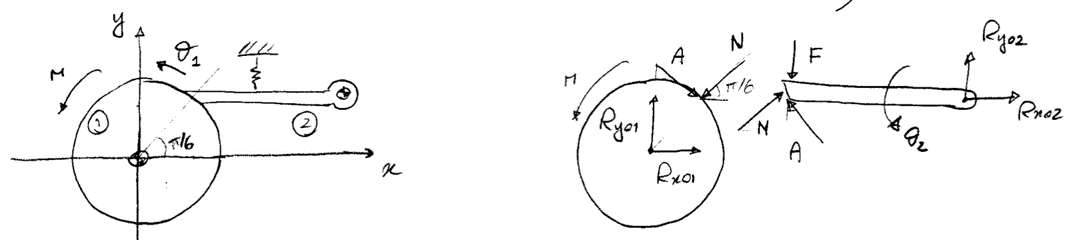
\includegraphics[width=.7\textwidth]{chapter05/Immagine180}
\end{center}

\begin{minipage}{.5\textwidth}
Corpo 1:
\[
\begin{dcases}
m\,\cancel{\ddot{x_1}} = R_{x01}\,-\,N\,\cos{\cfrac{\pi}{6}}\,+\,A\,\sin{\cfrac{\pi}{6}}\\
m\,\cancel{\ddot{y_1}} = R_{y01}\,-\,N\,\sin{\cfrac{\pi}{6}}\,-\,A\,\cos{\cfrac{\pi}{6}}\\
I_1\,\ddot{\theta_1} = M\,-\,A\,r
\end{dcases}
\]
\end{minipage}
\hfill
\begin{minipage}{.5\textwidth}
Corpo 2:
\[
\begin{dcases}
m\,\cancel{\ddot{x_2}} = N\,\cos{\cfrac{\pi}{6}}\,-\,A\,\sin{\cfrac{\pi}{6}}\,+\,R_{x02}\\
m\,\cancel{\ddot{y_2}} = N\,\sin{\cfrac{\pi}{6}}\,+\,A\,\cos{\cfrac{\pi}{6}}\,+\,R_{y02}\,-\,F\\
I_2\,\cancel{\ddot{\theta_2}} = F\,L\,-\,N\,\sin{\cfrac{\pi}{6}}\,L\,-\,A\,\sin{\cfrac{\pi}{6}}\,L
\end{dcases}
\]
\end{minipage}

Ci chiediamo in quali condizioni il freno possa mantenere fermo il tamburo: data la geometria del sistema e la forza F (che preme il ceppo contro il tamburo), ci sarà un momento oltre al quale il ceppo non riesce più a tenere fermo il tamburo e quindi quest'ultimo comincerà a muoversi.

Le condizioni di aderenza sotto le quali il sistema rimane fermo sono $\dot{\theta_1} = \dot{\theta_2} = 0$ e queste condizioni se sostituite nel sistema di equazioni di Newton-Eulero corrispondono alla soluzione statica, in cui tutto il sistema rimane fermo.

Per studiare questa condizione riprendiamo le equazioni di equilibrio alla rotazione del primo e del secondo corpo e imponiamo la condizione di staticità:
\[
\begin{dcases}
0 = M\,-\,A\,r\\
0 = F\,\cancel{L}\,-\,N\,\cfrac{1}{2}\,\cancel{L}\,-\,A\,\cfrac{\sqrt{3}}{2}\,\cancel{L}
\end{dcases}
\rightarrow
\begin{dcases}
A=\cfrac{M}{r}\\
N = 2\,F\,-\,\sqrt{3}\,A = 2F\,-\,\sqrt{3}\,\cfrac{M}{r}
\end{dcases}
\]
In condizioni statiche otteniamo queste due componenti A ed N e osserviamo che sono entrambe parametriche nel momento M: in particolare per il momento M=0 ci sarà un certo valore di azione normale N e l'attrito A è nullo; aumentando il momento M la forza d'attrito A tende ad aumentare, mentre la forza normale N tende a diminuire.

Proviamo a diagrammare la forza che il tamburo esercita sul ceppo in maniera parametrica con il momento M:

\begin{minipage}{.35\textwidth}
\centering
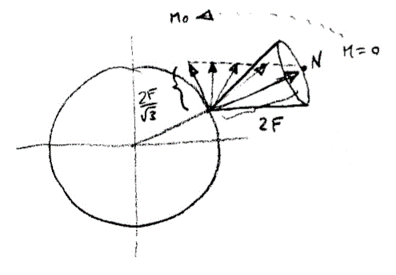
\includegraphics[width=.95\textwidth]{chapter05/Immagine181}
\end{minipage}
\hfill
\begin{minipage}{.65\textwidth}
All'aumentare del momento M si ha un aumento della componente tangenziale d'attrito A e una diminuzione della componente normale N, entrambe con un andamento di tipo lineare. Se diagrammassimo tutti i vettori risultanti dalle componenti N e A osserviamo che parametricamente con M vanno a descrivere un segmento.

Osserviamo anche una condizione in cui la forza normale arriva ad essere nulla e la forza d'attrito avrà un ben preciso valore: al fine di trovare tale condizione basta imporre N = 0.
\end{minipage}

Risolvendo rispetto a M, si ottiene che:
\[M_0 = \cfrac{2\,F\,r}{\sqrt{3}}\]
In queste condizioni il valore dell'attrito
\[A_0 = \cfrac{2\,F}{\sqrt{3}}\]
In questo diagramma abbiamo tutti i casi che matematicamente corrispondono all'equilibrio del sistema quindi all'aderenza delle superfici a contatto e abbiamo la descrizione di come varia la risultante al contatto al variare del momento motore che viene equilibrato.

Sappiamo tuttavia che al contatto tra due superfici non possono essere scambiate tutte le forze possibili, ma solamente quelle che stanno all'interno del cono di attrito statico hanno la possibilità di essere esercitate dal contatto; altrimenti si va a violare l'ipotesi di aderenza e si è in condizioni non più di staticità del sistema.

Sappiamo anche che il cono di attrito statico è descritto dall'equazione
\[\cfrac{A}{N} = f_a\qquad\Longrightarrow\qquad\cfrac{M}{r} = f_a\,(2\,F\,-\,\sqrt{3}\,\cfrac{M}{r})\qquad\Longrightarrow\qquad M = \cfrac{2\,f_a\,F\,r}{1\,+\,f_a\,\sqrt{3}} = M_{max}\]

Ci chiediamo cosa succede in condizioni di strisciamento.

Abbiamo varcato la soglia $M_{max}$ del momento motore e quindi il sistema non è più in condizioni statiche, ma in movimento.

La condizione che possiamo immediatamente scrivere è che il sistema, essendo in condizioni di strisciamento, la reazione vincolare non è più indeterminata all'interno del cono di attrito statico, ma giace sulla generatrice del cono di attrito dinamico. Quindi:
\[A = f_c\,N\]
Riscriviamo le equazioni di equilibrio alla rotazione dei due corpi, dove non possiamo più imporre che $\ddot{\theta_1} = 0$.
\[
\begin{dcases}
I_1\,\ddot{\theta_1} = M\,-\,f_c\,N\,r\\
0 = F\,L\,-\,N\,\cfrac{L}{2}\,-\,f_c\,N\,\cfrac{\sqrt{3}}{2}\,L
\end{dcases}
\]
Ottenendo le componenti di reazione vincolare
\[N = \cfrac{2\,F}{1\,+\,f_c\,\sqrt{3}}\qquad;\qquad A = \cfrac{2\,f_c\,F}{1\,+\,f_c\,\sqrt{3}}\]
A questo punto riprendiamo la prima equazione del moto, che è quella di interesse in quanto ci descrive l'accelerazione angolare del tamburo nelle condizioni in cui ci sia strisciamento:
\[I_1\,\ddot{\theta_1} = M\,-\,\cfrac{2\,f_c\,F\,r}{1\,+\,f_c\,\sqrt{3}}\]
Osserviamo che in generale M può dipendere dalle condizioni che imponiamo esternamente al tamburo e che quindi in generale il moto è un moto uniformemente accelerato.

Inoltre il valore del momento massimo che può essere equilibrato dall'attrito statico:
\[M = \cfrac{2\,f_a\,F\,r}{1\,+\,f_a\,\sqrt{3}}\]
Portando dunque il momento M al valore massimo ($M_{max}$) e lo varchiamo anche di un infinitesimo, il sistema si metterà in movimento. Sarà valida l'equazione del moto in condizioni di strisciamento: se manteniamo ora il momento al valore massimo osserviamo che l'accelerazione è proporzionale alla differenza dei due momenti e questa differenza non è zero perché $f_a > f_c$.

Da questo momento in poi pur mantenendo il momento pari al momento $M_{max}$, che ha permesso di mettere in moto il sistema, il moto risulta uniformemente accelerato.\newline

Ci occupiamo a questo punto di capire come funziona il freno all'inversione del verso del momento applicato al tamburo: ovvero quando esso opera nella configurazione di \textbf{ceppo compresso} e non più ceppo teso.

Riscriviamo le equazioni di equilibrio alla rotazione dei due corpi:
\[
\begin{dcases}
I_1\,\cancel{\ddot{\theta_1}} = -\,M\,+\,A\,r\\
I_2\,\cancel{\ddot{\theta_2}} = F\,\cancel{L}\,-\,N\,\sin{\cfrac{\pi}{6}}\,\cancel{L}\,+\,A\,\cos{\cfrac{\pi}{6}}\,\cancel{L}
\end{dcases}
\qquad
\begin{dcases}
A = \cfrac{M}{r}\\
N = 2\,F\,+\,\sqrt{3}\,\cfrac{M}{r}
\end{dcases}
\]

Osserviamo che le componenti di attrito e la componente normale sono ancora una volta funzioni del momento M, tuttavia A è sempre una funzione crescente del momento esattamente come l'espressione di N.

Al fine di individuare la risultante di queste due forze all'interno del cono di attrito statico, calcoliamo il rapporto tra componente tangenziale e componente normale:
\[\cfrac{A}{N} = \cfrac{\cfrac{M}{r}}{2\,F\,+\,\sqrt{3}\,\cfrac{M}{r}} = \cfrac{1}{\sqrt{3}\,+\,\cfrac{2\,F\,r}{M}} = \tan{\varphi}\]
Proviamo a vedere come al variare di M varia l'inclinazione di questa risultante e confrontiamo la risultante con il cono di attrito statico.

\begin{minipage}{.35\textwidth}
\centering
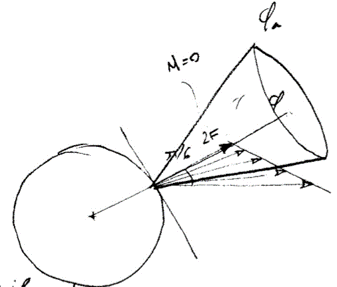
\includegraphics[width=.85\textwidth]{chapter05/Immagine182}
\end{minipage}
\hfill
\begin{minipage}{.65\textwidth}
In questo grafico, similmente a quanto realizzato per la condizione di ceppo teso riportiamo l'andamento della reazione vincolare al contatto con i due corpi, in particolare la forza che il tamburo esercita sul ceppo, in maniera parametrica rispetto al momento M che deve essere equilibrato dal contatto.

Quando il momento è nullo (M = 0), la componente di attrito A = 0  e si ha solo la componente normale N = 2 F.

Man mano che aumentiamo M, osserviamo che aumentano sia la componente normale che quella tangenziale in maniera lineare. La forza risultante quindi ha un andamento lineare.
\end{minipage}
\vspace{1mm}

Ci chiediamo cosa possa succedere a tale generica risultante della forza di contatto al variare del momento rispetto al cono di attrito statico diagrammato, che ha una semi-ampiezza pari all'angolo $\varphi_a$ (angolo di attrito statico).

Osserviamo che all'aumentare del momento l'inclinazione della risultante al contatto tende ad un valore asintotico:
\[\lim_{M \to \infty}\cfrac{\norma{A}}{\norma{N}} = \cfrac{1}{\sqrt{3}} = \tan{\varphi_{max}}\]
Da cui è possibile ricavare l'angolo di massima inclinazione della risultante rispetto alla normale
\[\varphi_{max} = \arctan{\cfrac{1}{\sqrt{3}}} = \cfrac{\pi}{6}\]
Sappiamo che l'ipotesi di aderenza vale fintanto che la reazione vincolare è interna al cono di attrito: a questo punto sapendo che l'inclinazione della risultante è un valore che passa da $\varphi = 0$ quando M = 0 e arriva a un valore $\varphi = \varphi_{max} = \cfrac{\pi}{6}$ la condizione di aderenza dipende da come si pone l'angolo $\varphi_a$ rispetto al valore $\varphi_{max}$.

Se la semiapertura del cono di attrito statico è maggiore o uguale a $\pi/6$ abbiamo che il cono di attrito conterrà sempre la risultante delle forze al contatto: il cono è più aperto di quanto possa essere inclinata la risultante al contatto rispetto alla normale e quindi per qualunque valore di momento si troverà in una situazione di equilibrio alle forze di contatto. Tale situazione è detta di \textbf{impuntamento}.

In questo caso il ceppo compresso non permette la rotazione del tamburo per quanto grande sia il momento applicato al tamburo stesso.

Se invece la semiapertura del cono di attrito è inferiore a $\pi/6$ ci sarà un valore di momento che porta l'inclinazione della risultante a stare sul cono di attrito statico e quindi aumentando ulteriormente il momento applicato al tamburo si passerà dalla condizione di aderenza alla condizione di strisciamento.

Per trovare tale condizione limite possiamo imporre che $\tan{\varphi_a} = \tan{\varphi}$ e di conseguenza:
\[\cfrac{1}{\sqrt{3}}{\cfrac{2\,F\,r}{M_max}} = \tan{\varphi_a}\]

\section{Lezione 29	-04 -- Daniele Bortoluzzi}

In questa lezione proseguiamo con lo studio dei componenti meccanici e in particolare continuiamo l'approfondimento di questi sistemi meccanici soprattutto per quel che riguarda i fenomeni che avvengono all'interfaccia tra i due corpi.

\begin{center}
{\scshape{\bfseries Esempio su aderenza e strisciamento}}
\end{center}

\begin{minipage}{.35\textwidth}
\centering
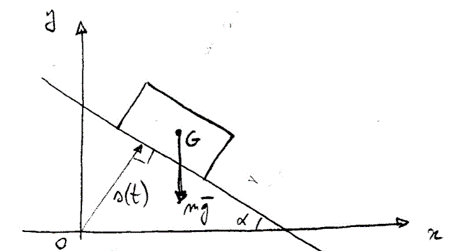
\includegraphics[width=.95\textwidth]{chapter05/Immagine183}
\end{minipage}
\hfill
\begin{minipage}{.65\textwidth}
Tale esercizio si avvale dell'attrito e in particolare del fatto che l'attrito, nella gran parte dei casi, è una funzione decrescente con la velocità di strisciamento per realizzare una sorta di sistema di movimentazione.

Immaginiamo di avere un piano inclinato sul quale appoggia un corpo soto l'effetto della gravità e delle forze di contatto tra corpo e piano inclinato di un angolo $\alpha$.
\end{minipage}
\vspace{1mm}

Il piano inclinato è azionato lungo la direzione ad esso ortogonale: quindi osserviamo una coordinata $s(t)$ tempo variante che viene comandata dall'esterno e osserviamo che c'è la possibilità di realizzare un sistema di trasporto e di movimentazione di questa massa regolando opportunamente questa legge del moto $s(t)$ e approfittando del fatto che al contatto tra corpo e piano inclinato si sviluppa un attrito di tipo Coulombiano (quindi ideale), che presenta un coefficiente di attrito statico superiore a quello di attrito cinetico.

Questo aspetto può permettere in modo molto semplice la movimentazione di questo corpo grazie all'effetto della gravità.

Prendiamo come legge del moto $s(t)$ di riferimento una legge armonica: $s(t) = a\,\sin{(\omega\,t)}$.

Cerchiamo il valore dell'ampiezza (a) oltre al quale il sistema non è più in condizione di aderenza e quindi inizia lo strisciamento relativo tra il corpo e il piano inclinato.

Per risolvere questo problema prendiamo un S.d.R. ruotato in cui l'asse delle ascisse è parallelo al piano inclinato e l'asse delle ordinate è ortogonale al piano inclinato, sempre centrato nell'origine del S.d.R. fisso.

In questo S.d.R. è particolarmente agevole scrivere le equazioni del moto perché siamo paralleli/perpendicolari alle componenti normali e di attrito che si sviluppano all'interfaccia tra i due corpi: il S.d.R. in questione $(x_r, y_r)$ è un sistema inerziale in quanto non è solidale al piano inclinato, ma è semplicemente orientato come il piano inclinato.

\begin{minipage}{.35\textwidth}
\centering
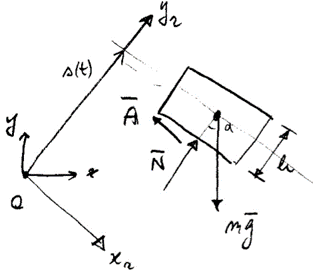
\includegraphics[width = .75\textwidth]{chapter05/Immagine184}
\end{minipage}
\hfill
\begin{minipage}{.65\textwidth}
Il piano inclinato, a sua volta, ha un movimento sinusoidale lungo la direzione $s(t)$ ortogonale al piano, però il S.d.R. $(x_r, y_r)$ rimane fisso.

In tale S.d.R. è possibile scrivere le equazioni del moto di un corpo assunto come punto materiale:
\[
\begin{dcases}
m\,\ddot{x_r} = m\,g\,\sin{(\alpha)}\,-\,A\\
m\,\ddot{y_r} = m\,g\,\cos{(\alpha)}\,+\,N
\end{dcases}
\]
\end{minipage}

Imponiamo l'ipotesi di  aderenza: ovvero che il sistema sia fermo rispetto al piano inclinato
\[\begin{dcases}
\dot{x_r} = 0\\
y_r = s(t)\,+\,\cfrac{h}{2}
\end{dcases}
\quad
\Longrightarrow
\quad
\begin{dcases}
\ddot{x_r} = 0\\
\ddot{y_r} = \ddot{s}(t) = -\,\omega^2\,a\,\sin{(\omega\,t)}
\end{dcases}\]

In questo caso stiamo risolvendo un problema di dinamica inversa: sappiamo qual è il moto del sistema nell'ipotesi di aderenza e dobbiamo trovare le forze che agiscono sul corpo stesso
\[\begin{dcases}
0 = m\,g\,\sin{(\alpha)}\,-\,A\\
-\,a\,\omega^2\,m\,\sin{(\omega\,t)} = -\,m\,g\,\cos{(\alpha)}\,+\,N 
\end{dcases}
\quad
\Longrightarrow
\quad
\begin{dcases}
A = m\,g\,\sin{(\alpha)}\\
N = m\,(g\,\cos{(\alpha)}\,-\,a\,\omega^2\,\sin{(\omega\,t)})
\end{dcases}
\]
A questo punto è necessario verificare che siano corrette tali soluzioni: bisogna trovare una relazione tra le grandezze in gioco che garantisca la validità dell'ipotesi di aderenza.

Sappiamo che il cono di attrito statico è definito dal coefficiente di aderenza $f_a$ e sappiamo che qualsiasi reazione vincolare all'interno del cono di attrito statico è possibile. In termini quantitativi possiamo scrivere la compatibiità di queste componenti tangenziale e normale con il cono di aderenza sulla base del loro rapporto:
\[\cfrac{\norma{A}}{\norma{N}}\,\le\,f_a\quad\Longrightarrow\quad\cfrac{\cancel{m}\,g\,\sin{(\alpha)}}{\cancel{m}\,(g\,\cos{(\alpha)}\,-\,a\,\omega^2\,\sin{(\omega\,t)})}\,\le\,f_a\]
Si noti che al fine di prendere la norma delle due componenti sappiamo che: nel caso della componente di attrito A sappiamo che possiamo prendere direttamente la sua espressione in quanto è sempre positiva, per quanto riguarda N lo riportiamo con l'espressione trovata, ma sarà necessario discutere l'espressione che ne risulta per comprenderne il campo di validità.

Per quanto riguarda il denominatore sappiamo che il vincolo che si realizza al contatto tra i due corpi è unilaterale e quindi ha senso tale rapporto solo quando il denominatore è positivo.

Se infatti sviluppiamo la disuguaglianza nell'ipotesi che il denominatore sia positivo otteniamo
\[g\,\cos{(\alpha)}\,-\,a\,\omega^2\,\sin{(\omega\,t)} \ge\,\cfrac{g}{f_a}\,\sin{(\alpha)}\]
Tale disequazione corrisponde alla validità dell'ipotesi di aderenza che abbiamo introdotto.
\[N(t) = m\,(g\,\cos{(\alpha)}\,-\,a\,\omega^2\,\sin{(\omega\,t)})\ge\,m\,\cfrac{g}{f_a}\,sin{(\alpha)}\]
Proviamo a interpretare la condizione di aderenza tramite un grafico:
\begin{center}
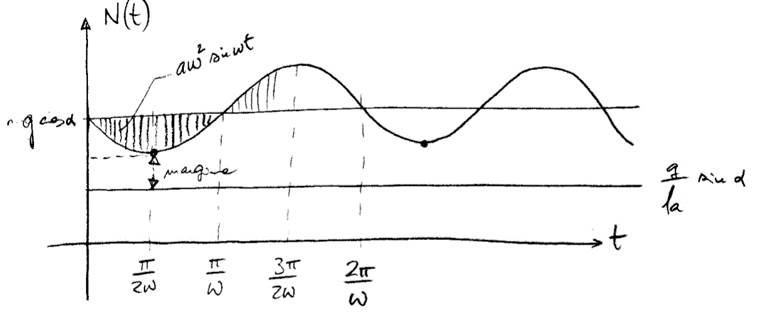
\includegraphics[width=.7\textwidth]{chapter05/Immagine185}
\end{center}
Osserviamo che è presente un termine costante ($m\,g\,\cos{\alpha}$) al quale sottraiamo il valore $(m\,a\,\omega^2\,\sin{(\omega\,t)})$, che ha un andamento sinusoidale.

Il risultato è ancora una funzione armonica con valore medio non nullo che dipende direttamente dalla massa, la costante di gravità e l'inclinazione del piano inclinato.

Tanto maggiore è l'inclinazione tanto più piccolo è questo valore medio e di conseguenza tanto più si abbassa il valore medio attorno al quale oscilla la funzione.

D'altra parte il valore sinusoidale ha un'ampiezza che dipende proporzionalmente da \emph{a} (moto imposto al piano inclinato) e quadraticamente dalla frequenza che imponiamo a movimento.

A questo punto confrontiamo l'andamento tempo variante con il valore soglia $(m\,\cfrac{g}{f_a}\,\sin{(\alpha)})$ che è tracciato come una retta orizzontale alla quota che gli compete: osserviamo che le condizioni di aderenza rimangono valide fintanto che l'andamento armonico diagrammato non interseca il valore di soglia.

Osserviamo anche che all'aumentare dell'angolo $\alpha$ diminuisce il valore medio e aumenta il valore di soglia: da un lato si alza il valore di soglia, dall'altro lato si abbassa il valore medio dell'oscillazione. In altri termini aumentando $\alpha$ ci si avvicina sempre più alle condizioni in cui si ha strisciamento incipiente, essendo il margine la distanza tra il minimo della funzione armonica e la soglia che abbiamo tracciato.

Pensando invece di aver fissato l'angolo di inclinazione del piano inclinato, possiamo avvicinarci o allontanarci dalle condizioni di strisciamento incipiente regolando l'ampiezza del moto imposto al piano inclinato oppure la frequenza; avendo però la frequenza un effetto molto più marcato (quadratico) sulla possibilità di far avvicinare la curva armonica al valore di soglia.

La condizione limite in cui rimane valida la condizone di aderenza si verifica quando la funzione armonica assume nel suo punto di minimo esattamente il valore di soglia.
\begin{align*}
N(t) &= m\,\cfrac{g}{f_a}\,\sin{\alpha}\\
 m\,(g\,\cos{(\alpha)}\,-\,a_{max}\,\omega^2\,\sin{(\omega\,t)})&=\,m\,\cfrac{g}{f_a}\,sin{(\alpha)}\\
 a_{max} &= \cfrac{1}{\omega^2}\,(g\,\cos{(\alpha)}\,-\,\cfrac{g}{f_a}\,\sin{(\alpha)})
\end{align*}
Questa applicazione ha senso quando si va a violare le condizioni di aderenza e quindi quando il sistema comincia a muoversi: pensando di aver fissato la frequeza da questa relazione si può trovare l'ampiezza oltre alla quale è opportuno far funzionere l'oscillatore affinché il movimento si abbia.

Lavorare sulla frequenza, tuttavia, è addirittura più efficace pensando che ha un effetto quadratico, ma aumentare in maniera indefinita la frequenza può non essere del tutto efficace perché benché l'attuatore possa essere in grado di produrre un moto alla frequenza desiderata, l'intero piano inclinato dovrebbe muoversi come un unico corpo rigido.

Questo non è detto che avvenga se si ha ripiani eccessivamente lunghe per cui la frequenza che andiamo a comandare può avvicinarsi ad una delle sue frequenze di risonanza: a quel punto la tavola vibrante non è più un corpo rigido e quindi tutta la trattazione fatta non è più valida.

\subsection{Meccanismi con elementi dotati di puro rotolamento}

Il problema di descrivere cosa succede tra corpi in movimento relativo si può porre anche all'interno di meccanismi e non solamente in corpi isolati come quello appena visto: non è infrequente il caso in cui anche all'interno di meccanismi (insieme di più corpi rigidi vincolati reciprocamente) si ponga il problema di descrivere il moto di rotolamento o strisciamento tra corpi.

Prendiamo il caso di puro rotolamento, che è un caso di riferimento spesso molto utile per capire il funzionamento di un meccanismo in condizioni nominali.

Consideriamo un corpo piano che rotola e ci poniamo il problema di descriverne il moto rispetto ad un S.d.R. Abbiamo di fatto un corpo a contatto con strisciamento, di conseguenza, un sistema a camma.

Dal calcolo dei G.d.L. di tale sistema composto da una ruota che si muove mantenendosi in contatto con un piano di riferimento possiamo applicare l'equazione di Grubler secondo la quale:
\[n = 3\,(2\,-\,1)\,-\,1\,1 = 2\,\text{G.d.L.}\]
Che corrispondono alla traslazione orizzontale e alla rotazione.

Posto che il moto della ruota è completamente descitto dal vettore $\und{\omega}$ e dalla velocità $\dot{x_c}$, andiamo a descivere la distribuzione delle velocità sulla ruota stessa.
\vspace{1mm}

\begin{minipage}{.25\textwidth}
\centering
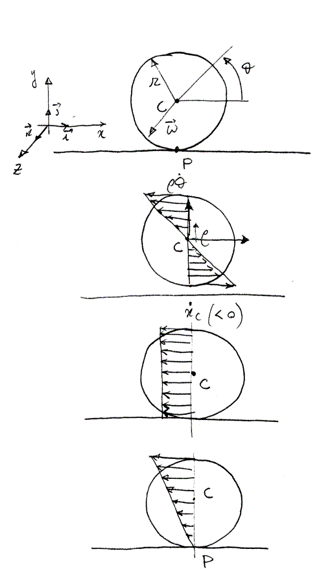
\includegraphics[width=.95\textwidth]{chapter05/Immagine186}
\end{minipage}
\hfill
\begin{minipage}{.75\textwidth}
Mettiamoci innanzitutto in un S.d.R. centrato in C e che quindi si muove con la ruota, ma non ruota: possiamo quindi la formula della velocità di un punto che appartiene ad un corpo rigido:
\[\und{\omega} = \dot{\theta}\,\cdot\,\mathbf{k}\qquad\mathbf{v} = \und{\omega}\wedge\und{\rho}\]
dove $\und{\rho}$ è il raggio vettore tra il centro e il punto generico.

Ci interessiamo per semplicità della distribuzione delle velocità dei punti lungo un diamentro della ruota orientato lungo l'asse y: il vettore $\und{\rho} = \rho\cdot\mathbf{j}$
\[\mathbf{v} = \dot{\theta}\cdot{k}\wedge\rho\,\mathbf{j} = -\,\rho\,\dot{\theta}\,\mathbf{i}\]
Abbiamo descritto la velocità di un punto generico di un corpo rigido (ruota) rispetto al S.d.R. centrato in C con assi paralleli a quelli fissi: la velocità in questione di conseguenza è una velocità relativa.

Possiamo sommare a questa velocità la velocità di trascinamento che per definizione è la velocità del punto generico del S.d.R. mobile che si sovrappone al punto di interesse, pensato invece solidale alla ruota.
\end{minipage}
\vspace{1mm}

Il moto di trascinamento è un moto di pura traslazione lungo l'asse x e quindi la velocità di trascinamento per tutti i punti della ruota è pari a
\[\mathbf{v} = (-\,\rho\,\dot{\theta}\,+\,\dot{x_C})\,\mathbf{i}\]
A questo punto osserviamo che sommando i due profili di velocità diagrammato in figura (uno con andamento a farfalla, l'altro invece costante) otteniamo un andamento, in generale, a farfalla traslato a seconda di come sono le velocità angolari e la velocità di trascinamento.

La condizione di puro rotolamento si ha quando il punto di contatto tra la ruota e il terreno ha velocità nulla: imponendo che la velocità del punto di contatto P sia pari a zero, si ottiene una relazione che esprime il fatto di avere un moto di puro rotolamento del nostro corpo.

Per ottenere la velocità $v_P$ del punto della ruota a contatto con il suolo, sostituiamo a $\rho$ il valore $\rho_P = -\,r$ (ricordiamo che $\rho$ è positivo verso la direzione positiva di y, mentre il punto P è identificato da una coordinata $\rho$ negativa).
\[v_P = r\,\dot{\theta}\,+\,\dot{x_C} = 0\]
Da cui possiamo ricavare una relazione tra le grandezze $\dot{\theta}$ e $\dot{x_C}$.
\begin{gather*}
\int \dot{x_C} = \int -\,r\,\dot{\theta}\\
x_C = -\,r\,\theta\,+\,cost.
\end{gather*} 
Questa relazione cinematica che esprime la condizione di puro rotolamento della ruota in un piano è rappresentata da una relazione di vinolo sulle velocità: ciò implica che il vincolo di puro rotolamento è un vincolo \textbf{non olonomo} o \textbf{anolonomo}, in quanto è espresso come una funzione delle derivate delle coordinate generalizzate e non delle coordinate generalizzate stesse.

Tuttavia in questo caso il vincolo matematico è facilemente integrabile: pur essendo espresso nelle velocità questo vincolo, per le condizioni di puro rotolamento nel piano, può essere integrato ed espresso sulle coordinate generalizzate.

\subsection{Rotolamento puro oppure con strisciamento}

Si ricorda che il fatto che si realizzi rotolamento puro oppure a strisciamento tra i corpi è un problema dinamico: è quindi necessario scrivere le equazioni del moto per capire se al contatto tra due corpi si realizza una condizione oppure l'altra.
\begin{center}
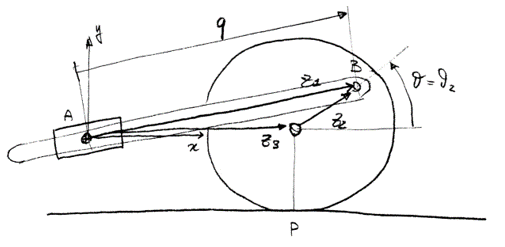
\includegraphics[width=.7\textwidth]{chapter05/Immagine187}
\end{center}

Come cinematica possiamo solo scrivere condizioni per le quali esiste una relazione tra le velocità dei corpi quando ci sia il moto di puro rotolamento, ma per verificare se ci sia o meno la condizione di puro rotolamento bisogna coinvolgere la dinamica dei corpi a contatto.

Prendiamo come esempio un meccanismo che preveda la presenza di una ruota posta a contatto con un piano: scriviamo semplicemente la cinematica di questo sistema che prevede un corpo in rotolamento.

Partiamo dall'ipotesi che non sappiamo a priori se ci sia o meno strisciamento fra le superfici e scriviamo le equazioni della cinematica per questo sistema.

Il sistema presenta una ruota a cui è collegata una biella e questa scorre su un pattino che ha il centro vincolato da una coppia rotoidale a telaio.

Scriviamo l'equazione cinematica mediante il poligono di chiusura:

\begin{gather*}
q\,\B{\cos{\theta_1}\\\sin{\theta_1}}\,-\,a_2\,\B{\cos{\theta_2}\\\sin{\theta_2}}\,-\,a_3\,\B{\cos{\theta_3}\\\sin{\theta_3}} = \B{0\\0}\\
q\,\B{\cos{\theta_1}\\\sin{\theta_1}}\,-\,a_2\,\B{\cos{\theta_2}\\\sin{\theta_2}}\,-\,\B{x_C\\y_C} = \B{0\\0}
\end{gather*}

In cui le incognite sono $\theta_1, \theta_2$ e $x_C$, una voltascelta come coordinata generalizzata \emph{q}.

Possiamo osservare che questo sistema di 2 equazioni in 3 incognite non ammette soluzione in quanto si ha sovrabbondanza di incognite rispetto alle equazioni del sistema.

L'indeterminatezza del sistema di equazioni sta proprio nel fatto che non abbiamo fatto alcuna considerazione sulla natura del contatto tra ruota e terreno, in quanto non abbiamo ipotizzato le condizioni di puro rotolamento.

Sappiamo quindi che quando un vincolo può essere espresso in termini delle coordinate generalizzate e non delle sue derivate si dice \textbf{vincolo olonomo} ($f(x_C,\theta)$), mentre quando ciò non è possibile si dice \textbf{vincolo non olonomo o anolonomo} ($f(\dot{x_c},\dot{\theta})$).

Nel nostro caso pur avendo un'espressione del tipo $f(\dot{x_C},\dot{\theta}) = 0$, mediante semplice integrazione è possibile ricondurre il vincolo non olonomo ad un'espressione di vincolo olonomo.

La costante di integrazione dell'espressione equivalente olonoma si trova note le condizioni iniziali del meccanismo, che possono essere ad esempio: la coordinata $x_C = x_{C0}$ quando $\theta = 0$.

Introduciamo ora l'ipotesi di puro rotolamento al meccanismo: che tale ipotesi sia o meno vera rimane una questione da verificare in base alla dinamica una volta trovata la soluzione trovata dal puro rotolamento. Sulla base di forze e momenti che agiscono sul sistema si trovano le reazioni vincolari (componente normale e tangenziale) e si verifica che nelle condizioni di moto si mantiene vera l'ipotesi che la reazione vincolare rimane all'interno del cono di attrito statico.

Qualora ciò non valga più anche la cinematica del sistema viene a cambiare in quanto non vale più la relazione tra $x_C$ e $\theta$ derivante dal moto di puro rotolamento.

Di conseguenza, limitandoci esclusivamente al calcolo cinematico di questo sistema e introducendo l'ipotesi di puro rotolamento, per il quale:
\[x_C = -\,r\,\theta\,+\,x_{C0}\]
riscriviamo le equazioni della cinematica:
\[q\,\B{\cos{\theta_1}\\\sin{\theta_1}}\,-\,a_2\,\B{\cos{\theta_2}\\\sin{\theta_2}}\,-\,\B{x_C\\y_C} = \B{0\\0}\]
A questo punto le incognite che rimangono sono $\theta_1$ e $\theta_2$ dal momento che fissato q come coordinata generalizzata è possibile risolvere il sistema perché l'incognita $x_C$ è espressa in funzione di $\theta_2$.

\subsection{Componenti meccanici: ruote di frizione}

Passiamo ora a vedere alcune componenti meccanici, in particolare \textbf{le ruote di frizione}. In questa trattazione cercheremo di essere più generali e trovare una relazione che ci esprima la massima coppia che può essere espressa dalla ruota motrice alla ruota condotta.
\begin{center}
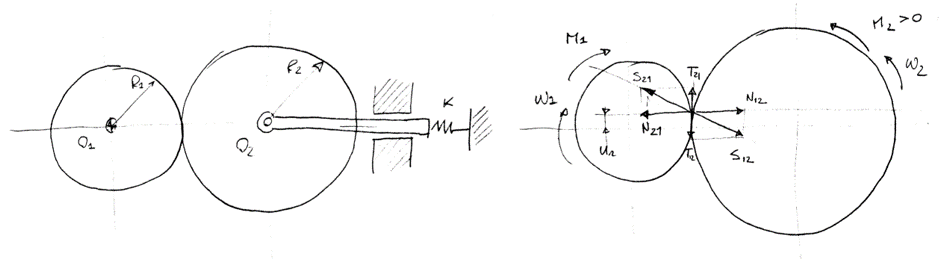
\includegraphics[width=.7\textwidth]{chapter05/Immagine188}
\end{center}

Consideriamo un sistema in cui è presente:
\begin{itemize}
\item una \textbf{ruota motrice} vincolata al telaio tramite una coppia rotoidale e di raggio $R_1$
\item una \textbf{ruota condotta} di raggio $R_2$ e origine $O_2$, posta a contatto con la ruota motrice e mantenuta a contatto da una forza che è prodotta esternamente al sistema mediante una molla
\item una \textbf{molla precaricata} che mantiene la ruota condotta a contatto con la ruota motrice.
\end{itemize}
Inoltre sono presenti un momento motore $M_1$ applicato alla ruota motrice e un momento resistente $M_2$ alla ruota condotta.

Ci interessa trovare l'espressione del massimo momento che può essere trasmesso dalla ruota motrice alla ruota condotta in assenza di strisciamento.

Lo schema proposto presenta componenti normali che non sono più localizzate al punto di intersezione del segmento che unisce i due centri, ma è spostato: questo perché ci aspettiamo che ci sia un certo attrito di rotolamento (che sarà espresso da un certo parametro di attrito che descriverà di quanto si sposta in avanti la reazione normale e quindi decrive in maniera implicita il momento di rotolamento che si oppone al moto di rotazione).

\begin{minipage}{.29\textwidth}
\centering
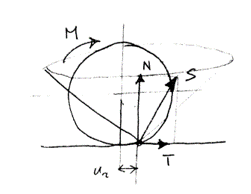
\includegraphics[width=.85\textwidth]{chapter05/Immagine189}
\end{minipage}
\hfill
\begin{minipage}{.71\textwidth}
Ridisegnando una ruota che ha moto di rotolamento su una superficie andiamo a disegnare la componente tangenziale di attrito T, la componente normale di reazione vincolare N (la quale come abbiamo anticipato non è localizzato nel piano di simmetria della ruota, ma anticipa il movimento della ruota stessa), la reazione vincolare S (composizione delle due precedenti azioni) e il cono di attrito localizzato nel punto dove si ha la risultante delle pressioni.
\end{minipage}

L'assenza di strisciamento si imporrà come l'appartenenza della reazione vincolare S al più al cono o al suo interno. Sotto tali ipotesi vale la relazione cinematica di uguale velocità dei punti a contatto reciproco tra le due ruote, ovvero il rapporto di trasmissione:
\[\tau = \cfrac{\omega_2}{\omega_1} = -\,\cfrac{R_1}{R_2}\]
Dove il segno negativo sta a indicare che rispetto alle convenzioni le ruote hanno velocità angolari opposte.

Ci occupiamo ora di trovare la massima coppia trasmissibile: essendo la coppia legata alla componente tangenziale, cioè alla componente d'attrito, è intuitivo che la massima coppia si avrà quando la reazione vincolare S si trova sulla generatrice del cono. In altri termini quando:
\[T = f\,N\]

Studiamo il funzionamento delle due ruote di frizione nelle condizioni limite, ovvero quando la reazione vincolare giace sul cono di attrito statico e ci riferiamo alle condizioni in cui le due ruote hanno velocità angolari costanti (accelerazioni angolari nulle).

Ipotizziamo che non siano presenti strisciamenti anche a livello microscopico, cioè anche l'impronta nel contatto tra le due ruote non ha nessun fenomeno dissipativo rilevante: in queste condizioni possiamo scrivere un modello molto semplice, ma utile a capire l'efficacia di questo tipo di trasmissione.

Scriviamo quindi per la ruota motrice l'equazione di Eulero, per cui essendo l'accelerazione angolare nulla, tutti i momenti si compensano:
\[
\begin{dcases}
M_ = N_{21}\,u_r\,+\,f\,N_{21}\,R_1 = N_{21}\,(u_r\,+\,f\,R_1)\\
M_2=N_{12}\,(u_r\,-\,f\,R_2)
\end{dcases}
\]
Abbiamo ottenuto due espressioni per i due momenti; possiamo imporre che $N_{12} = N_{21} = N$ in quanto sono semplici reazioni l'una rispetto all'altra e le due equazioni che ritornano $M_1$ e $M_2$ mettono in relazione i momenti motore e frenante al coefficiente di attrito, il parametro di attrito di rotolamento e la forza N (carico con cui noi forziamo le due ruote l'una contro l'altra).

Si possono utilizzare queste due equazioni per trovare la forza N, nota $M_2$:
\[N = \cfrac{M_2}{u_r\,-\,f\,R_2}\] 
Oppure è possibile trovare la $M_2$ massima trasmissibile avendo fissato un certo precarico N tra le due ruote.

Troviamo, in questo modo, anche la reazione S completa:
\[\norma{S} = \sqrt{(f\,N)^2\,+\,N^2} = N\,\sqrt{f^2\,+\,1}=M_2\,\cfrac{\sqrt{f^2\,+\,1}}{u_r\,-\,f\,R_2}\]
Può essere utile calcolare il rendimento di questo sistema. Tale sistema è finalizzato a traferire una certa coppia $M_1$ dal motore alla ruota condotta secondo una certa relazione, che idealmente è legata solo ai raggi delle due ruote.
\[M_2 = N\,(u_r\,-\,f\,R_2) = M_1\,\cdot\,\cfrac{u_r\,-\,f\,R_2}{u_r\,+\,f\,R_1}\]
E questo è il momento che troviamo alla ruota condotta in condizioni reale.

In condizioni ideali
\[M^*_2 = -\,M_1\,\cfrac{R_2}{R_1}\]
In assenza di qualsiasi altro fenomeno dissipativo il rendimento può essere calcolato come:
\[\eta = \cfrac{M_2}{M_2^*}=\cfrac{ \cancel{M_1}\,\cdot\,\cfrac{u_r\,-\,f\,R_2}{u_r\,+\,f\,R_1}}{ -\,\cancel{M_1}\,\cfrac{R_2}{R_1}} = \cfrac{-\,\cfrac{u_r}{R_2}\,+\,f}{\cfrac{u_r}{R_1}\,+\,f}\]

Fino ad ora abbiamo considerato condizioni di funzionamento al limite dell'aderenza in cui la forza che si scambiano le due ruote sta sul cono di attrito statico.

Adesso proviamo a considerare le condizioni in cui il momento che trasmettiamo viene ridotto rispetto alle condizioni limite di aderenza: la riduzione di momento sia a $M_1$ che a $M_2$ porta la reazione vincolare ad essere interna al cono di attrito statico in una condizione che dipende dai momenti motore e frenante applicati al sistema.

Consideriamo il sistema in funzionamento con stesso precarico N e riscriviamo le equazioni di equilibrio delle due ruote, avendo sempre condizioni di funzionamento di regime (accelerazioni angolari nulle):
\[
\begin{dcases}
M_1 = N_{21}\,(u_r\,+\,f\,R_1)\\
M_2 = N_{12}\,(u_r\,-\,f\,R_2)
\end{dcases}
\]
Qualora \emph{f} corrisponda al coefficiente di aderenza o attrito statico, siamo nelle condizioni limite nelle quali $T = f\,N$.

Pensiamo invece a condizioni di funzionamento generiche di aderenza, ma non al limite: la componente tangenziale di forza T al contatto tra le due superfici è minore ($T < f\,N$). Posto che possiamo sempre riferirci al rapporto tra T e N con un coefficiente, che appunto è legato all'angolo di cui la risultante si allontana dalla normale, possiamo scrivere che in generale:
\[T = f^*\,N\]
dove $f^*$ è una generica condizione di attrito statico all'interno del relativo cono di attrito, tale che ($f^* < f$), e dipenderà dai momenti $M_1$ e $M_2$ che stiamo applicando al sistema compatibilmente con il fatto che l'accelerazione angolare delle ruote sia pari a zero.

Detto questo possiamo ripercorrere lo stesso calcolo che abbiamo fatto precedentemente, riferito alle condizioni di aderenza, e arrivare ad un'espressione del rendimento (formalmente identica a quella di prima) in cui il coefficiente \emph{f} non è più il coefficiente di aderenza, ma è il coefficiente generico $f^*$ che si riferisce alle condizioni di funzionamento interne al cono di aderenza.
\[\eta^* = \cfrac{-\,\cfrac{u_r}{R_2}\,+\,f^*}{\cfrac{u_r}{R_1}\,+\,f^*}\]
Si osservi che $u_r$ è rimasta invariata in quanto il parametro di attrito di rotolamento è sostanzialmente funzione del precarico N, avendo le stesse ruote con stesse caratteristiche di elasticità e di proprietà del materiale al contatto rispetto a quelle del caso precedente e avendo ottenuto l'espressione di N uguale al caso precedente.

Dallo studio delle espressione dei due rendimenti concludiamo che $\eta^* < \eta$. Pertanto il rendimento di una coppia di ruote di frizione diminuisce quando si lavora in condizioni diverse da quella di aderenza limite: l'utilità/efficacia di questo tipo di trasmissione si ha quando le coppie sono sufficientemente alte da far funzionare il sistema in condizione di aderenza limite.

Osseviamo inoltre che se trasmettiamo un coppia molto bassa, si può arrivare ad ottenere un rendimento $\eta^* = 0$.

Mentre quando $f^* < \cfrac{u_r}{R_2}$ il rendimento diventa negativo: il significato di questa condizione è che se applichiamo una coppia troppo piccola il sistema non riesce a muoversi.
L'effetto della componente normale N combinato con il braccio (parametro di attrito di rotolamento) $u_r$ è sufficiente ad equilibrare l'effetto della coppia che applichiamo.

La soluzione a questo problema è quella di adeguare il precarico N alla coppia da trasmettere, in particolare: se ci troviamo a trasmettere una coppia che va diminuendo è opportuno diminuire in maniera concorde anche il precarico N. La riduzione del precarico N porta ad una riduzione del parametro di attrito di rotolamento $u_r$ e, di conseguenza, il fattore detrimentale che abbiamo al numeratore e al denominatore.

In questo modo il rendimento non risente più di tanto della riduzione del momento in quanto si trova a lavorare sempre in prossimità della condizione di aderenza.

\section{Lezione 06-05 -- Daniele Bortoluzzi}

\subsection{Esercizio: sospensione McPherson}

\begin{minipage}{.5\textwidth}
\centering
\includegraphics[width=.9\textwidth]{chapter05/Immagine191}
\end{minipage}
\hfill
\begin{minipage}{.5\textwidth}

In questa lezione trattiamo un esercizio che è un meccanismo piano che costituisce il meccanismo alla base della sospensione McPherson, la quale è una delle più diffuse in campo automobilistico.

È un esercizio che si pone l'obiettivo di trattare la cinematica e la dinamica di un meccanismo e costituisce un utile momento di ripasso dei metodi già visti a lezione per risolvere meccanismi a catena chiusa.

Il meccanismo è costituito da tre corpi:
\begin{itemize}
\item il membro \textbf{AC} vincolato a telaio dalla cerniera A
\item il membro \textbf{CD} collegato con una coppia prismatica al corpo rigido vincolato a telaio nella coppia B e con una coppia rotoidale al corpo AC.
\item il telaio
\end{itemize}
\end{minipage}

Ci sono  dunque tre coppie rotoidali (A, B, C) e una coppia prismatica che collega il corpo rigido \textbf{CD} al corpo vincolato a telaio in B. 

In questa configurazione il meccanismo costituisce un meccanismo di sospensione di un autoveicolo in cui si pensa che la ruota sia vincolata in D e ruoti attorno ad un asse complanare al meccanismo e orintato secondo l'asse x: durante il movimento del veicolo, nel S.d.R. solidale al telaio del veicolo stesso, la ruota a causa dell'irregolarità del terreno si dovrà spostare lungo l'asse y e lo faccia secondo la risposta di questo meccanismo, pensato per questo scopo.

Si richiede di:
\begin{enumerate}
\item Trovare il rapporto di trasmissione tra lo spostamento verticale del punto D ($y_D$) e la rotazione del mozzo (CD). Tale rapporto di trasmissione indica quanto il movimento verticale della sospensione provochi anche una rotazione dell'asse attorno al quale ruota lo pneumatico. 

La direzione CD, che nello schema è parallela all'asse x, opportuno che lo rimanga il più possibile durante il funzionamento della sospensione.
\item Trovare l'accelerazione del braccetto (CD) quando sul pneumatico agisce una forza verticale \textbf{F} in condizione di velocità nulla, nell'ipotesi che sia una massa concentrata nel centro di massa D.

L'ipotesi dunque è che la ruota rappresenti una massa concentrata nel punto D, che il meccanismo sia inizialmente fermo e che ad un certo putno riceva una forza verticale (a rappresentare l'interazione del pneumatico con l'asfalto).
\end{enumerate}

Cominciamo con la prima delle due domande:

Prendiamo come coordinate generalizzate la rotazione $\theta_1$ del braccio AC e la rotazione $\theta_2$ del braccio CB. Considereremo poi la rotazione $\theta_1$ come movente del meccanismo e tutte le altre grandezze come cedenti.

Essendo un meccanismo piano a catena chiusa risolviamo questo problema mediante il poligono di chiusura:
\begin{gather*}
\mathbf{AC} + \mathbf{CB} + \mathbf{BA} = 0\\
r\,\B{\cos{\theta_1}\\\sin{\theta_1}}\,+\,(L\,+\,s)\,\B{\cos{\theta_2}\\\sin{\theta_2}}\,+\,h\,\B{0\\-1} = 0
\end{gather*}

dove \emph{s} è una grandezza che varia a seconda della configurazione del meccanismo e costituisce anch'essa un'incognita della cinematica.

Riscrivendo le due equazioni in forma scalare:
\[
\begin{dcases}
r\,\cos{\theta_1}\,+\,(L+s)\,\cos{\theta_2} = 0\\
r\,\sin{\theta_1}\,+\,(L+s)\,\sin{\theta_2}\,-\,h=0
\end{dcases}
\]
Procediamo ora al calcolo dei rapporti di velcoità. Per far questo derivamo le due equazioni rispetto al tempo e raccogliamo nella matrice Jacobiana i coefficienti delle derivate delle incognite $\dot{\theta_2}, \dot{s}$ avendo portato a secondo membro i termini che contengono la coordinata movente $\dot{\theta_1}$.
\[
\M{\cos{\theta_2}&-\,(L\,+\,s)\,\sin{\theta_2}\\\sin{\theta_2}&(L\,+\,s)\,\cos{\theta_2}}\,\B{\dot{s}\\\dot{\theta_2}} = r\,\B{\sin{\theta_1}\\-\,\cos{\theta_1}}\,\dot{\theta_1}
\]
D'ora in poi consideriamo $q = \theta_1$.

Calcoliamo il determinante della matrice jacobiana:
\[Det[J] = (L\,+\,s)\,\cos^2{\theta_2}\,+\,(L\,+\,s)\,\sin^2{\theta_2} = L\,+\,s\]
Quindi il vettore $\tau$ contenente i due rapporti di velocità:
\[\B{\tau} = \M{\cos{\theta_2}&\sin{\theta_2}\\-\,\cfrac{\sin{\theta_2}}{L+s}&\cfrac{\cos{\theta_2}}{L+s}}\,r\,\B{\sin{q}\\\cos{q}}=\B{r\,\sin{(q-\theta_2)}\\-\,\cfrac{r}{L+s}\,\cos{(q-\theta_2)}}\]
Per cui i rapporti di velocità risulteranno essere:
\begin{gather*}
\tau_{q\,\theta_2} = -\,\cfrac{r}{L+s}\,\cos{(q-\theta_2)}\\
\tau_{y_C\,\theta_2} = \cfrac{\dot{\theta_2}/\dot{q}}{\dot{y_C}/\dot{q}} = \cfrac{\tau_{q\,\theta_2}}{\tau_{q\,y_C}}
\end{gather*}

Ricordo che il risultato del vettore dei rapporti di velocità dipende direttamente da come abbiamo definito il vettore delle velocità incognite quando abbiamo scritto le equazioni della cinematica. $\B{\dot{s}\\\dot{\theta_2}}$.

Dal rapporto di velocità sopra riportato, dunque, conosciamo solo il termine al numeratore. Possiamo tuttavia trovare il termine al denominatore dal momento che la coordinata q muove l'intero meccanismo:
\[\mathbf{AC} = r\,\B{\cos{q}\\\sin{q}}\qquad;\qquad \mathbf{v_C}=\td{\mathbf{AC}}{t} = r\,\B{-\,\sin{q}\\\cos{q}}\,\dot{q}\]
Da cui
\[\dot{y_C} = r\,\cos{q}\,\dot{q} = \tau_{q\,y_C}\,\dot{q}\]
A questo punto sostituendo tale rapporto di velocità nell'espressione che abbiamo travato:
\[\tau_{y_C\,\theta_2} = -\,\cfrac{\cancel{r}}{L+s}\,\cos{(q-\theta_2)}\,\cfrac{1}{\cancel{r}\,\cos{q}}\]
che rappresenta il rapporto tra la rotazione del mozzo e la velocità di spostamento verticale della ruota.

Possiamo osservare che le potenziali configurazioni singolari di questo meccanismo si ottengono per $s = - L$, ma affinché ciò avvenga il punto C dovrà arrivare a coincidere con il punto B. In questa realizzazione pratica la cosa è impossibile pertanto possiamo dire che nelle condizioni di funzionamento previste per questo cinematismo questo non raggiunge mai la configurazione singolare.

È opportuno tuttavia che il rapporto di velocità calcolato sia minimizzato in quanto solo in questo modo garantiamo che durante il funzionamento della sospensione, l'asse di rotazione della ruota non venga modificato in direzione, ma che trasli mantenendosi parallelo alla configurazione iniziale.

Una volta ottenuto il rapporto di velocità tra spostamento verticale del punto C e rotazione del mozzo è possibile chiedersi se esistono delle condizioni ideali di funzionamento di questo meccanismo.

Dal momento che sappiamo che la rotazione rispetto allo spostamento verticale sia nulla in un caso ideale:
\[\tau_{y_C\,\theta_2} = 0 \quad\Longrightarrow\quad \cos{(q-\theta_2)} = 0 \quad\Longrightarrow\quad q-\theta_2 = \cfrac{\pi}{2}\,+\,k\,\pi\] 

\begin{center}
\includegraphics[width=.7\textwidth]{chapter05/Immagine192}
\end{center}

Se osserviamo il significato geometrico di questa condizione si ottiene che tale condizione è verificata quando l'asta AC è ortogonale all'asta BC; tra le configurazioni matematicamente compatibili con l'annullamento del rapporto di velocità esiste quella in cui $\theta_2\,-\,q = \cfrac{\pi}{2}$ (k = -1).

A cavallo di questa condizione un piccolo spostamento verticale della ruota non comporta alcuna rotazione essendo il rapporto di velocità nulla. Se impostiamo l'angolo tra l'asta CD e l'asta CB pari all'angolo $\theta_2$ in questa configurazione, il braccetto CD si trova orizzontale e rimarrà tale anche per piccoli spostamenti verticali del punto D.

In questa cofigurazione abbiamo dunque un'idealità di funzionamento lungo l'asse verticale (y), ciò non toglie che pur ruotando la ruota possa muoversi lungo una traiettoria che preveda anche componenti orizzontali di spostamento; abbiamo sì annullato la rotazione dell'asta CD (asse di rotazione della ruota), però il punto D può combinare una componente verticale di spostamento con una componente orizzontale (che costituirà un funzionamento non ideale in quanto origina strisciamento dello pneumetico nella direzione dell'asse).

Il secondo punto a cui rispondere è di trovare l'accelerazione del braccetto supponendo che sullo pneumatico agisca una forza verticale \textbf{F} con meccanismo inizialmente fermo e nell'ipotesi che l'unica inerzia agente sul sistema sia una massa agente sull centro della ruota D.

In questo senso il meccanismo è particolarmente semplice in quanto è possibile trovarne l'accelerazione utilizzando il PLV:

Scriviamo il vettore AD come somma di vettori AC e CD di cui quest'ultimo visto come somma di un angolo fisso e di un angolo variabile nel suo intorno.
\[\mathbf{AD} = r\,\B{\cos{q}\\\sin{q}}\,+\,l\,\B{\cos{(\theta_2-\und{\theta_2})}\\\sin{(\theta_2-\und{\theta_2})}}\]
Differenziamo l'espressione trovata per trovare lo spostamento virtuale del punto D, noto che in questa configurazione il meccanismo non ha rotazioni dei corpi ($\delta \theta_2 = 0$):
\[\delta\mathbf{D} = r\,\B{-\,\sin{q}\\\cos{q}}\,\delta q\,+\,l\,\B{-\,\sin{(\theta_2\,-\,\und{\theta_2})}\\\cos{(\theta_2\,-\,\und{\theta_2})}}\cancelto{0}{\delta \theta_2} = r\,\B{-\,\sin{q}\\\cos{q}}\,\delta q\]

Come accennato in precedenza è necessario calcolare l'accelerazione del punto D dove è localizzata l'unica massa del sistema in modo da poter calcolare la forza d'inerzia e con questa bilanciare la forza esterna agente sullo pneumatico.

La forza d'inerzia risulterà proporzionale all'accelerazione del punto D, pertanto riprendiamo il calcolo dello spostamento virtuale del punto D dove abbiamo sviluppato il differenziale del vettore AD e aggiungiamo la derivata temporale:
\[\mathbf{a_D} = r\,\B{-\,cos{q}\\-\,\sin{q}}\,\dot{q}^2\,+\,r\,\B{-\,\sin{q}\\\cos{q}}\,\ddot{q}\,+\,l\,\cancelto{0}{\B{-\,\cos{(\theta_2-\und{\theta_2})}\\-\,\sin{(\theta_2-\und{\theta_2})}}\,\dot{\theta_2}}\,+\,l\,\B{\cancelto{0}{-\,\sin{(\theta_2-\und{\theta_2})}}\\\cancelto{1}{\cos{(\theta_2-\und{\theta_2})}}}\,\ddot{\theta_2}\]
In questa formulazione generale dobbiamo inserire le ipotesi del calcolo che si riferiscono alla condizioni in cui consideriamo il meccanismo ovvero la condizione in cui la rotazione $\theta_2$ è stazionaria e di conseguenza lo spostamento virtuale del meccanismo a cavallo di questa configurazionenon provoca rotazione.

Possiamo ipotizzare dunque che $\dot{\theta_2} = \dot{q} = 0$.

Alla luce delle ipotesi appena enunciate possiamo calcolare il vettore tra \textbf{AP}, dove P è il putno di contatto tra pneumatico e asfalto, trattandolo come somma vettoriale:
\[\mathbf{AP} = \mathbf{AD}\,+\,\mathbf{DP} = \mathbf{AD}\,+\,R\,\B{\sin{(\theta_2+\und{\theta_1})}\\-\cos{(\theta_2-\und{\theta_2})}}\]
Noto il vettore \textbf{AP} possiamo calcolare il suo spostamento virtuale al fine di calcolare il lavoro virtuale della forza di contatto:
\[\delta \mathbf{P} = \delta \mathbf{D}\,+\,R\,\B{\cos{(\theta_2-\und{\theta_2})}\\\sin{(\theta_2-\und{\theta_2})}}\cancelto{0}{\delta \theta_2} = \delta \mathbf{D}\]
Calcoliamo ora il lavoro virtuale delle forze agenti sul sistema: il lavoro virtuale nel caso in esame risulta essere:
\[\delta L_{virt} = \mathbf{F}\cdot\delta\mathbf{P} \,+\,\mathbf{F}_{inerzia}\,\cdot\delta\mathbf{D} = 0\]
dove:
\begin{itemize}
\item \[\mathbf{F}\cdot\delta \mathbf{P} = \B{0\\F}\cdot r\,\B{-\,\sin{q}\\\cos{q}}\delta q = F\,r\,\cos{q}\,\delta q\]
\item \begin{align*}
\mathbf{F}_{inerzia}\cdot\delta \mathbf{D} &= -\,m\,\mathbf{a_D}\,\delta \mathbf{D} = (-\,m\,r\,\B{-\,\sin{q}\\\cos{q}}\ddot{q}\,+\,l\,\B{0\\1}\,\ddot{\theta_2})\cdot r\,\B{-\,\sin{q}\\\cos{q}}\,\delta q\\
&= -\,m\,r^2\,\sin{q}\,\ddot{q}\,\sin{q}\,\delta q\,+\,(-\,m\,r\,\cos{q}\,\ddot{q}\,+\,l\,\ddot{\theta_2})\,r\,\cos{q}\,\delta q
\end{align*}
\end{itemize}
Ci interessa a questo punto mettere in relazione l'accelerazione $\ddot{\theta_2}$ con la configurazione del meccanismo e le caratteristiche di velocità. Quindi riportare alla coordinata libera e alla configurazione del meccanismo tutte le variabili che compaiono nell'espressione.

Partendo dalla definizione di rapporto di velocità:
\[\dot{\theta_2} = \tau_{q\,\theta_2}\,\dot{q} = -\,\cfrac{r}{L+s}\,\cos{(q-\theta_2)}\,\dot{q}\]
Derivando ulteriormente nel tempo:
\[\ddot{\theta_2} = -\,r\,\cfrac{(-\,\sin{(q-\theta_2)}(\dot{q}-\dot{\theta_2})\,\cancel{\dot{q}}\,+\,\cos{(q-\theta_2)}\ddot{q})\,(L+s)\,+\,\cos{(q-\theta_2)}\,\dot{q}\cancel{\dot{s}}}{(L+s)^2}\] 
Applicando le condizioni di riferimento: $\dot{q} = 0$, $\dot{\theta_2} = 0$, $\dot{s} = 0$, si ottiene l'espressione dell'accelerazione:
\[\ddot{\theta_2} = -\,\cfrac{r}{(L+s)^{\cancel{2}}}\,\cos{(q-\theta_2)}\,\ddot{q}\,\cancel{(L+s)} = -\,\cfrac{r}{L+s}\,\cancelto{0}{\cos{(q-\theta_2)}}\,\ddot{q} = 0\]
Sostituendo tutte le espressioni ottenute nell'espressione del lavoro virtuale:
\begin{align*}
\delta L_{virt} &= F\,r\,\cos{q} \delta q\,-\,m\,r^2\,\sin^2{q}\,\ddot{q}\,\delta q\,-\,m\,r^2\,\cos^2{q}\,\ddot{q}\,\delta q\\
&= F\,\cancel{r}\,\cos{q}\,\delta q \,-\,m\,r^{\cancel{2}}\,\ddot{q}\,\delta q = 0
\end{align*}
Da questo bilancio di lavori virtuali possiamo esplicitare l'accelerazione della coordinata libera:
\[\ddot{q} = \cfrac{F}{m\,r}\,\cos{q}\]

Al di là  del risultato matematico si può cercare di dare un'interpretazione fisica a questo risultato:

\begin{minipage}{.5\textwidth}
Vediamo che nella configurazione di riferimento la forza applicata al punto D può essere scomposta in due componenti (ortogonale e parallela alla direzione del braccio BC, lungo la quale il braccio CD si sta muovendo). Pertanto l'accelerazione del sistema può essere trovata come rapporto tra la forza e la massa:
\[a = \cfrac{F\,\cos{q}}{m} = \ddot{q}\,r\]
Ottenendo esattamente l'accelerazione del putno materiale D per effetto dell'accelerazione della coordinata libera q.
\end{minipage}
\hfill
\begin{minipage}{.5\textwidth}
\centering
\includegraphics[width=.95\textwidth]{chapter05/Immagine193}
\end{minipage}

\subsection{Componenti meccanici: Trasmissioni a cinghia}

Le trasmissioni a cinghia sono molto frequenti nell'ambito dell'ingegneria meccanica per cui è utile trovare delle relazioni che descrivino il loro funzionamento, in particolare la coppia che possiamo trasmettere con una trasmissione a cinghia in funzione delle caratteristiche principali (coefficiente di attrito, elasticità della cinghia, velocità angolare della puleggia...).

Prendiamo un modello ideale di cinghia in cui quest'ultima si avvolge per un certo angolo sulla puleggia come indicato in figura e partiamo da un'analisi infinitesima dinamica della cinghia per arrivare poi ad un'espressione più generale che coinvolge l'intera cinghia nella sua interazione con la puleggia (ci permetterà di trovare il momento trasmesso da questo tipo di trasmissione).

\begin{center}
\includegraphics[width=.65\textwidth]{chapter05/Immagine194}
\end{center}

Estraiamo un elemento infinitesimo di cinghia a cui è associato un certo angolo di curvatura (che è lo stesso della puleggia) e su questo elemento infinitesimo definiamo una coordinata curvilinea \emph{s} lungo la circonferenza media nello spessore della cinghia, definiamo anche un S.d.R. centrato nell'elemento infinitesimo di cinghia composto da un asse normale che punta verso il centro della puleggia e un asse tangenziale che punta verso sinistra.

Vengono riportate anche le forze che agiscono su questo elemento infinitesimo di cinghia in modo da evidenziarne la loro differente natura:
\begin{itemize}
\item Forze normali $\mathbf{F_n}$ che sono forze per unità di lunghezza della cinghia e sono le pressioni che si sviluppano al contatto tra cinghia e puleggia e che quindi tendono a spingere l'elemento infinitesimo di cinghia verso l'esterno.
\item Azioni tangenziali al contatto tra puleggia e cinghia legate all'attrito $\mathbf{F_t}$, e sono sostanzialmente delle pressioni (forze per unità di lunghezza) anche se si riferiscono a componenti di forza che stanno sulla superficie di contatto invece che perpendicolari. Sono orientate nello stesso verso dell'asse t.
\item Forze che l'elemento infinitesimo di cinghia riceve lungo le superfici che lo collegano alla parte restante di cinghia $\mathbf{R}$. Esse sono funzioni della posizione della coordinata \emph{s} e sono in generale diverse tra una superficie e l'altra dell'elemento infinitesimo di cinghia di lunghezza \emph{ds}.
\end{itemize}

Scriviamo le equazioni del moto di questo elemento infinitesimo di cinghia in modo vettoriale, ovvero scriviamo che la somma di tutte le forze che agiscono su questo elemento infinitesimo di cinghia sono uguali alla massa (sia $\mu$ la densità lineare di massa [Kg/m]) per la sua accelerazione:
\[
\mu\,ds\,\mathbf{a} = \mathbf{F}\,ds\,+\,(\cancel{\mathbf{R}} + d\mathbf{R}) - \cancel{\mathbf{R}}
\]
Sviluppando la funzione R(s) e esprimendone il differenziale 
\[d\mathbf{R} = \pd{\mathbf{R}}{s}\,ds\]
e sostituendo tale espressione al bilancio di forze:
\begin{align*}
\mu\,\cancel{ds}\,\mathbf{a} &= \mathbf{F}\,\cancel{ds}\,+\,\pd{\mathbf{R}}{s}\,\cancel{ds}\\
\mu\,\mathbf{a} = \mathbf{F}\,+\,\pd{\mathbf{R}}{s}
\end{align*}

L'equazione così ottenuta è indefinita in quanto non si riferisce ad un ben definito elemento di cinghia, ma è generica dell'elemento inifinitesimo che può essere posizionato ovunque lungo l'arco di contatto tra cinghia e puleggia.

Scriviamo ora le componenti \textbf{R} e \textbf{F}:
\[\mathbf{R}(s) = T\,\mathbf{t}\qquad;\qquad \mathbf{F}(s) = -\,F_n\,\mathbf{n}\,+\,F_t\,\mathbf{t}\]
Scriviamo ora la velocità della cinghia $\mathbf{v} = v\,\mathbf{t}$, e al fine di calcolare l'accelerazione che è presente nell'equazioni indefinita dell'equilibrio calcoliamo la derivata di questo vettore velocità:
\begin{align*}
\mathbf{a} &= \td{v}{t}\,\mathbf{t}\,+\,v\,\td{\mathbf{t}}{t} = \td{v}{t}\,\mathbf{t} \,+\,v\,(\und{\omega_C}\wedge\mathbf{t})\qquad (\text{il prodotto esterno è }\parallel \mathbf{n})\\
&= \td{v}{t}\,\mathbf{t}\,+\,v\,\omega_C\,\mathbf{n} = \td{v}{t}\,\mathbf{t}\,+\,\cfrac{v^2}{r}\,\mathbf{n}\qquad\qquad(\omega = \cfrac{v}{r})
\end{align*}
Introdurremmo in seguito l'ipotesi che la cinghia in moto stazionario è inestensibile pertanto la derivata della velocità nel tempo sarà pari a zero.

Torniamo ora all'equazione indefinita di equilibrio dell'elemento infinitesimo di cinghia e osserviamo che oltre all'accelerazione compare un termine legato alla derivata della tensione rispetto a \emph{s}.
\[\pd{\mathbf{R}}{s} = \pd{}{s}(T\,\mathbf{t}) = \pd{T}{s}\,\mathbf{t}\,+\,T\,\pd{\mathbf{t}}{s}\]

\begin{minipage}{.5\textwidth}
dove:
\[\mathbf{t} = \cos{\theta}\,\mathbf{i}\,-\,\sin{\theta}\,\mathbf{j}\]
noto dalla figura a finaco che $\theta = s/r$
\[\mathbf{t} = \cos{\cfrac{s}{r}}\,\mathbf{i}\,-\,\sin{\cfrac{s}{r}}\,\mathbf{j}\]
In questo modo sarà possibile eseguire la derivata rispetto alla coordinata curvilinea del vettore tangente
\[\pd{\mathbf{t}}{s} = -\,\sin{\cfrac{s}{r}}\,\cfrac{1}{r}\,\mathbf{i}\,-\,\cos{\cfrac{s}{r}}\,\cfrac{1}{r}\,\mathbf{j} = -\,\cfrac{1}{r}\,(\sin{\theta}\,\mathbf{i}\,+\,\cos{\theta}\,\mathbf{j})\]
Dove l'argomento tra parantesi non è altro che il versore - \textbf{n}.
\end{minipage}
\hfill
\begin{minipage}{.5\textwidth}
\centering
\includegraphics[width=.95\textwidth]{chapter05/Immagine195}
\end{minipage}

Così facendo è finalmente possibile esprimere la derivata parziale di \textbf{R} rispetto alla coordinata curvilinea \emph{s}.
\[\pd{\mathbf{R}}{s}=\pd{T}{s}\,\mathbf{t}\,+\,\cfrac{T}{R}\,\mathbf{n}\]
Così facendo, sostituiamo i termini calcolati precedentemente nell'equazioni indefinita di equilibrio:
\[\mu\,\cancel{\td{v}{t}}\,\mathbf{t}\,+\,\mu\,\cfrac{v^2}{r}\,\mathbf{n}=-\,F_n\,\mathbf{n}\,+\,F_t\,\mathbf{t}\,+\, \pd{T}{s}\,\mathbf{t}\,+\,\cfrac{T}{r}\,\mathbf{n}\]
Per ogni versore della terna fissata possiamo scrivere un'equazione di equilibrio:
\[\mu\,\cfrac{v^2}{r} = -\,F_n\,+\,\cfrac{T}{r}\qquad;\qquad F_t\,+\,\pd{T}{s}=0\]
dove le incognite risultano essere $T, F_n, F_t$ (3 incognite in 2 equazioni).

Non è ancora possibile trovare una soluzione in forma chiusa in quanto mancano informazioni: non abbiamo la possilbità di risolvere il sistema.

L'informazione che manca è la presenza di un legame tra le forze tangenziali e le forze normali, ovvero la presenza di una legge di attrito tra la componente tangenziale di forza e quella normale.

Introduciamo questo legame sapendo che esistono due possibilità: 
\begin{enumerate}
\item L'elemento infinitesimo di cinghia non stia scorrendo sulla puleggia e che quindi sia in condizioni di aderenza/attrito statico, nel qual caso vale una relazione di disuguaglianza del tipo:
\[\norma{F_t}\le f_s\,F_n\]
con $f_s$ attrito statico

L'uguaglianza è valida solo in condizioni di moto incipiente.
\item L'elemento infinitesimo di cinghia è soggetto a scivolamento:
\[\norma{F_t} = f\,F_n\]
Il sistema è quindi definito.
\end{enumerate}

Quale di queste due condizioni si verifichi al momento non è ancora definito: ci accorgeremo tuttavia che a causa della deformabilità della cinghia sarà inevitabile concludere che l'elemento infinitesimo di cinghia scivoli rispetto alla puleggia e, di conseguenza, sarà opportuno introdurre la seconda equazione:
\[F_t = \pm f\,F_m\]
La distinzione di segno risiede nei casi in cui la puleggia sia motrice (+) o condotta (-).

\section{Lezione 13-05 -- Daniele Bortoluzzi}

Proseguiamo alla trattazione delle cinghie di trasmissione e all'espressione della massima coppia trasmissibile, quindi la coppia che porta la cinghia a lavorare alle condizioni limite dell'aderenza.

Ci focalizziamo dunque sulle condizioni di massima coppia trasmessa: all'interno del cono di attrito statico sappiamo di essere localizzati sulla generatrice del cono, per cui vale l'uguaglianza stretta
\[F_t = \pm f_s\,F_n\]
Il fatto che ci sia la dualità di segno dipende da come si proietta la risultante $F_t$ rispetto al S.d.R. preso ($\mathbf{t}, \mathbf{n}$): in particolare se la $F_t$ è equiversa a $\mathbf{t}$ le forze di attrito  tra la puleggia e la cinghia stanno promuovendo il moto della cinghia nella direzione positiva (antioraria) e quindi la ruota che abbiamo in esame è una ruota motrice.

Se invece la forza tangenziale che la puleggia sta esercitando sulla cinghia è opposta a $\mathbf{t}$, e quindi si oppone al senso antiorario preso come positivo per la rotazione e il momento, implica che la ruota è una ruota condotta.

Portiamo di conseguenza avanti il calcolo con entrambi i segni ricordando tale differenza.

Riportiamo le due equazioni di interesse (normale e tangenziale):
\[\mu\,\cfrac{v^2}{r} = -\,F_n\,+\,\cfrac{T}{r}\qquad;\qquad F_t\,+\,\pd{T}{s} = 0\]
Facciamo l'ipotesi semplificativa che la forza centrifuga $\mu\,\cfrac{v^2}{r}$ sia trascurabile. Questo permette di scrivere il sistema di equazioni:
\[
\begin{dcases}
F_n = \cfrac{T}{r}\\
F_t\,+\,\pd{T}{s} = 0
\end{dcases}
\]
Dalla seconda equazione possiamo esplicitare la derivata della tensione rispetto a \emph{s} e introduciamo la condizione di massima coppia trasmissibile (interazione puleggia-cinghia al limite dell'aderenza):
\[\pd{T}{s} = -\,F_t = \mp\,f_s\,F_n=\mp\,f_s\,\cfrac{T}{r}\]
Riorganizzando gli estremi dell'equazione differenziale:
\[\pd{T}{s}\,\pm\,f_s\,\cfrac{T}{r}=0\qquad\Longrightarrow\qquad T = c\,e^{\mp\,\cfrac{f_s}{t}\,s}\]

\begin{minipage}{.5\textwidth}
Per ottenere il valore di \emph{c} è necessario imporre le condizioni al contorno di questo problema differenziale:
\[s= 0\qquad\quad T = T_1\]

\begin{itemize}
\item Motrice:
\[T_2 = T_1\,e^{-\,f_s\,\cfrac{s_2}{r}} = T_1\,e^{-\,f_s\,\alpha}\]
\item Condotta:
\[T_2 = T_1\,e^{f_s\,\cfrac{s_2}{r}} = T_1\,e^{f_s\,\alpha}\]
\end{itemize}
\end{minipage}
\hfill
\begin{minipage}{.5\textwidth}
\centering
\includegraphics[width=.7\textwidth]{chapter05/Immagine196}
\end{minipage}
\vspace{1mm}

Dal punto di vista applicativo è utile arrivare ad un'espressione della coppia trasmissibile nelle condizioni che abbiamo identificato (ovvero di strisciamento incipiente): sappiamo infatti che in condizioni in cui avvenisse lo scivolamento la forza tangenziale è ottenibile mediante il coefficiente di attrito cinetico, che tuttavia è inferiore a quello di aderenza e quindi possiamo aspettarci che la coppia trasmessa sia inferiore.

Per trovare la coppia integriamo lungo l'angolo $\alpha$, lungo il quale si ha il contatto tra puleggia e cinghia, i contributi infinitesimi di momento che sono $F_t\,ds\,r$:
\begin{align*}
M &= \int_{\alpha}\,F_t\,r\,ds\qquad\text{ma } F_t = -\,\pd{T}{s}\\
&= \int_{\alpha}-\,\pd{T}{s}\,r\,ds = r\,(T_1\,-\,T_2)
\end{align*}
In questa espressione si osservano due elementi di tensione simbolici che in realtà sono legati dalla legge esponenziale ricavata in precedenza:
\[M = r\,(T_1\,-\,T_2) = r\,(T_2\,e^{f\,\alpha}\,-\,T_2) = r\,T_2\,(e^{f\,\alpha}\,-\,1)\]
In questo caso stiamo considerando la condizione di puleggia motrice.

Si possono fare alcune considerazioni molto utili mediante la formulazione appena trovata:
\begin{enumerate}
\item Per aumentare la coppia trasmessa da puleggia motrice a cinghia è necessario avere elevati di \emph{f} e $\alpha$
\item Per aumentare il momento trasmesso si può aumentare l'angolo di avvolgimento $\alpha$ che ovviamente è legato ai raggi delle due pulegge e all'eventuale presenza di dispositivi che permettano di aumentarlo: un galoppino, ovvero una puleggia folle che è utilizzato per aumentare l'angolo tra cinghia e puleggia, forzando il ramo lento/meno teso ad avvolgersi di più lungo la puleggia stessa.
\item Il momento è proporzionale alla tensione $T_2$ sul ramo lento/meno teso: questo ci dice che non possiamo mai avere una trasmissione in cui la tensione sul ramo lento è nulla perché questo porterebbe immancabilmente ad avere nullo anche la coppia trasmissibile.
\end{enumerate}

\subsection{Esercizio}

Vediamo ora un esercizio su un meccanismo piano a più catene cinematiche che ci permette di ripassare la cinematica e la dinamica dei meccanismi piani.

Il meccanismo mostrato in figura è composto da:

\begin{minipage}{.5\textwidth}
\centering
\includegraphics[width=.95\textwidth]{chapter05/Immagine197}
\end{minipage}
\hfill
\begin{minipage}{.5\textwidth}
\begin{itemize}
\item un primo corpo rigido (guida prismatica) vincolata a telaio nell'origine del S.d.R. \textbf{OD}, e ruota attorno alla coppia rotoidale O di un angolo pari a \emph{q}.

È presente anche un corsoio/pattino localizzato nel punto D.
\item una seconda guida prismatica vincolata a telaio da una cerniera in C, \textbf{CF}.

È presente un corsoio che si muove localizzato nel punto E.
\item un terzo corpo rigido vincolato a telaio nel punto B sul quale sono presenti due coppie cinematiche rotoidali nei punti D e E che sono connesse ai pattini che scorrono nelle due guide prismatiche
\end{itemize}
\end{minipage}
\vspace{2mm}

Il sistema è costituito da più catene cinematiche e quindi richiede di essere studiato con i metodi già visti in precedenza.

Partiamo dall'analisi del numero di G.d.L. del sistema: la formula di Grubler ci dice che 
\[n = 3\,(m\,-\,1)\,-\,2\,c_1\,-\,c_2\]
Abbiamo due modi per calcolare il numero di G.d.L. di questo meccanismo:
\begin{enumerate}
\item Un primo approccio prevede di trattare le coppie cinematiche in D e in E, dove coincidono coppie prismatiche e rotoidali, come una coppia a camma.

Prendiamo ad esempio il corsoio in E: osserviamo che il pattino si muove lungo la guida CF, sul quale è localizzata una coppia rotoidale.

Allo stesso modo nel punto D coincidono la guida prismatica e la coppia rotoidale.

Seguendo questo approccio:
\[n = 3\,(4\,-\,1)\,-\,2\cdot3\,-\,2 = 1\,\text{G.d.L.}\]
\item Possiamo risolvere questo calcolo utilizzando un altro approccio in cui separiamo le coppie cinematiche che geometricamente coincidono.

In D e in E coincidono due coppie (un pattino e una cerniera); idealmente separando tutte le coppie cinematiche in questione permette di osservare che tra le coppie separate persiste un corpo di dimensione (teoricamente) nulla.
\[n = 3\,(6\,-\,1)\,-\,2\cdot7 = 1\,\text{G.d.L.}\]
\end{enumerate}

Procediamo al calcolo cinematico del meccanismo: essendo un meccanismo piano a più catene chiuse ci orientiamo verso la scrittura dei poligoni di chiusura delle varie catene cinematiche che possiamo identificare.

È utile per scrivere tali equazioni individuare i percorsi più semplici che descrivono il legame cinematico (quindi geometrico) tra i vari membri del meccanismo; ad esempio osserviamo che sono presenti le catene cinematiche:
\[\mathbf{OB} + \mathbf{BD}  - \mathbf{OD} = 0\qquad;\qquad \mathbf{BC}  + \mathbf{CE} -\mathbf{BE} = 0\]
A questo punto scriviamo in maniera simbolica le due equazioni vettoriali di chiusura delle due catene cinematiche, osservando che tutte le lunghezze fisse sono tra le coppie rotoidali a telaio è pari a \textbf{L}:

\begin{minipage}{.65\textwidth}
\[L\,\B{0\\1}\,+\,L\,\B{\cos{\theta}\\\sin{\theta}}\,-\,s\,\B{\cos{q}\\\sin{q}}=0\]
\[L\,\B{0\\1}\,+\,s_2\,\B{\cos{\theta_2}\\\sin{\theta_2}}\,-\,2\,L\,\B{\cos{\theta}\\\sin{\theta}} = 0\]
\end{minipage}
\hfill
\begin{minipage}{.3\textwidth}
\centering
\includegraphics[width=.95\textwidth]{chapter05/Immagine198}
\end{minipage}

Osserviamo a questo punto che le due catene cinematiche sono \textbf{debolmente accoppiate}, cioè possiamo risolvere la prima catena cinematica senza coinvolgere la seconda nel calcolo perché se osserviamo la prima equazione vettoriale, data la coordinata generalizzata \emph{q} è possibile calcolare immediatamente le due grandezze cinematiche incognite della prima catena cinematica (\emph{s} e $\theta$).

In particolare la coordinata $\theta$ sarà quella da sostituire alla seconda catena cinematica per risolvere rispetto alle ultime due incognite cinematiche ($s_2$ e $\theta_2$).

Come seconda richiesta è stato imposto di trovare le velocità del meccanismo in funzione della velocità di \emph{q} in una configurazione assegnata ($q = \pi / 4$).

In questo caso dobbiamo procedere derivando le equazioni di chiusura a cascata:
\begin{enumerate}
\item Prima catena cinematica
\[
\begin{dcases}
-\,L\,\sin{\theta}\,\dot{\theta}\,+\,s\,\sin{q}\,\dot{q}\,-\,\cos{q}\,\dot{s} = 0\\
L\,\cos{\theta}\,\dot{\theta}\,-\,s\,\cos{q}\,\dot{q}\,-\,\sin{q}\,\dot{s} = 0
\end{dcases}
\]
L'espressione è lineare nelle derivate delle coordinate ed è quindi possibile scriverla sotto forma di prodotto tra matrici:
\[\M{-\,L\,\sin{\theta}&-\,\cos{\theta}\\L\,\cos{\theta}&\,\sin{q}}\,\B{\dot{\theta}\\\dot{s}} = \,\B{-\,s\,\sin{q}\\s\,\cos{q}}\,\dot{q}\] 
\item Seconda catena cinematica
\[
\begin{dcases}
-\,s_2\,\sin{\theta_2}\,\dot{\theta_2}\,+\,\cos{\theta_2}\,\dot{s_2}\,+\,2\,L\,\sin{\theta}\,\dot{\theta} = 0\\
s_2\,\cos{\theta_2}\,\dot{\theta_2}\,+\,\sin{\theta_2}\,\dot{s_2}\,-\,2\,L\,\cos{\theta}\,\dot{\theta} = 0
\end{dcases}
\]
In questo secondo sistema di equazioni procediamo in maniera analoga a prima, individuiamo la coordinata libera e la portiamo a secondo membro: in questo caso abbiamo visto che, grazie al fatto che il meccanismo è debolmente accoppiato, possiamo risolvere la prima catena cinematica rispetto a $\theta$ e quindi, in questo secondo meccanismo i termini in $\theta$ e $\dot{\theta}$ possono essere portati a secondo membro e considerati moventi della seconda catena cinematica.
\[\M{-\,s_2\,\sin{\theta_2}&\cos{\theta_2}\\s_2\,\cos{\theta_2}&\sin{\theta_2}}\,\B{\dot{\theta_2}\\\dot{s_2}} = \B{-\,2\,L\,\sin{\theta}\\2\,L\,\cos{\theta}}\,\dot{\theta}\]
\end{enumerate}

\begin{minipage}{.5\textwidth}
A questo punto abbiamo espresso il problema cinematico in due problemi risolvibili a cascata in cui: la velocità della coordinata libera \emph{q} produce le velocità $\dot{s}$ e $\dot{\theta}$,  tra le quali quest'ultima può essere sostituita nella seconda catena cinematica per trovarne le rispettive velocità.

Per risolvere il problema si possono invertire le due matrici Jacobiane oppure sostituire la configurazione assegnata, sostituirli negli Jacobiani e invertire gli Jacobiani una volta fatta la sostituzione.
\end{minipage}
\hfill
\begin{minipage}{.5\textwidth}
\centering
\includegraphics[width=.95\textwidth]{chapter05/Immagine199}
\end{minipage}

In questo caso la configurazione assegnata ($q = \pi/4$) ha una cinematica particolarmente semplice da risolvere: si può risolvere infatti mediante semplici considerazioni geometriche sullo schema del meccanismo: osserviamo che in corrispondenza di questa coordinata del movente, grazie la fatto che \textbf{OB} e \textbf{BD} sono uguali, il triangolo è un triangolo rettangolo e isoscele per cui la lunghezza \textbf{OD} (che è la coordinata \emph{s}) si calcola facilmente come  $L\,\sqrt{2}$.

La prima catena cinematica è dunque risolta osservando la configurazione assegnata. Per quanto riguarda la seconda catena cinematica osserviamo che, essendo l'angolo $\measuredangle OBD$ pari a $\pi / 2$ il membro \textbf{BE}, quindi si è ottenuto il triangolo BCE rettangolo per cui il calcolo dell'ipotenusa ($L\,\sqrt{5}$) che l'angolo $\measuredangle BCE$ ($\arctan{2}$) è immediato.

Sostituiamo dunque nei due sistemi di equazioni la configurazione che abbiamo trovato per risolverli rispetto alle velocità del meccanismo:
\begin{align*}
\M{-\,L\,\sin{\theta}&-\,\cos{\theta}\\L\,\cos{\theta}&\,\sin{q}}\,\B{\dot{\theta}\\\dot{s}} = \,\B{-\,s\,\sin{q}\\s\,\cos{q}}\,\dot{q}\qquad&;\qquad\M{-\,s_2\,\sin{\theta_2}&\cos{\theta_2}\\s_2\,\cos{\theta_2}&\sin{\theta_2}}\,\B{\dot{\theta_2}\\\dot{s_2}} = \B{-\,2\,L\,\sin{\theta}\\2\,L\,\cos{\theta}}\,\dot{\theta}\\
\M{-\,L &-\,\cfrac{1}{\sqrt{2}}\\0&-\,\cfrac{1}{\sqrt{2}}}\,\B{\dot{\theta}\\\dot{s}} = \B{-\,L\\L}\,\dot{q}\qquad&;\qquad\M{-\,2\,L&-\,\cfrac{1}{\sqrt{5}}\\-\,L&\cfrac{2}{\sqrt{5}}}\,\B{\dot{\theta_2}\\\dot{s_2}} = \B{-\,2\,L\,\dot{\theta}\\0}\\
\B{\dot{\theta}\\\dot{s}} = \B{2\,\dot{q}\\-\,\sqrt{2}\,L\,\dot{q}}\qquad&;\qquad\B{\dot{\theta_2}\\\dot{s_2}} = \B{\cfrac{4}{5}\,\dot{\theta}\\\cfrac{2\,L}{\sqrt{5}}\,\dot{\theta}} = \B{\cfrac{8}{5}\,\dot{q}\\\cfrac{4\,L}{\sqrt{5}}\,\dot{q}}
\end{align*}

La terza richiesta coinvolge le azioni agenti sul meccanismo, in particolare viene richiesto di  trovare, nella configurazione assegnata, il momento $M_0$ per equilibrare un momento $M_B$.

\begin{minipage}{.7\textwidth}
L'ipotesi che vengono date è di meccanismo in presenza di vincoli lisci e meccanismo fermo che significa velocità e accelerazioni nulle.

Possiamo risolvere molto facilmente il problema applicando il principio dei lavori virtuali per il quale i lavori virtuali di tutte le azioni presenti sul sistema è pari a 0.
\end{minipage}
\hfill
\begin{minipage}{.25\textwidth}
\centering
\includegraphics[width=.95\textwidth]{chapter05/Immagine200}
\end{minipage}

A cavallo della configurazione assegnata gli spostamenti virtuali del sistema portano tutte le azioni a svolgere un lavoro complessivamente nulo:
\[\delta L = M_0 \,\delta q\,+\,M_B\,\delta \theta = 0\]
In questa espressione troviamo l'incognita $M_0$ che è pari a:
\[M_0 = -\,M_B\cfrac{\delta \theta}{\delta q} = -\,M_B\,\tau_{q\,\theta}\]
Il rapporto di velocità è stato ricavato nell'analisi cinematica tramite poligono di chiusura nel punto precedente:
\[\tau_{q\,\theta} = \cfrac{\dot{\theta}}{\dot{q}} = \cfrac{2\,\dot{q}}{\dot{q}} = 2\]
Di conseguenza:
\[M_0 = -\,2\,M_B\]

Il punto seguente richiede di trovare la reazione vincolare esericitata in E in condizione di equilibrio quando una forza \textbf{P} è esercitata in direzione orizzontale al punto F nella configurazione assegnata.

Per trovare la risposta a questa domanda osseviamo che per trovare l'equilibrio di questo sistema complessivo garantendo l'equilibrio dell'asta \textbf{CF} sulla quale sono applicate le forze in oggetto quindi: prendendo la forza \textbf{P} e osserviamo che viene equilibrata dalla sola reazione presente nella coppia prismatica in E e C, disassemblando il meccanismo, otteniamo la possibilità di mettere in equilibrio un sottosistema del meccanismo che ci permette di trovare le incognite in forma chiusa.

\begin{minipage}{.7\textwidth}
Sull'asta \textbf{CF}, disassemblata dal meccanismo, sono applicate:
\begin{itemize}
\item la forza \textbf{P} applicata al punto F;
\item la reazione vincolare $\mathbf{R_E}$ applicata al punto E 
\item le reazioni vincolari $\mathbf{R_{Cx}}$ e $\mathbf{R_{Cy}}$ applicata alla coppia rotoidale a telaio in C
\end{itemize}
\end{minipage}
\hfill
\begin{minipage}{.25\textwidth}
\centering
\includegraphics[width=.95\textwidth]{chapter05/Immagine201}
\end{minipage}

Osserviamo che la direzione della reazione interna, essendo il vincolo ideale (la coppia prismatica è priva di attrito), è possibile assumerla ortogonale all'asta \textbf{CF}.

Per mettere in equilibrio l'asta in esame possiamo scrivere 3 equazioni (equilibrio alla traslazione orizzontale, verticale e alla rotazione), inoltre possiamo osservare che può essere particolarmente agevole scrivere le equazioni di equilibrio alla rotazione scegliendo opportunamente il polo in maniera tale da minimizzare le incognite che abbiamo nel calcolo.

Se infatti scriviamo tale equilibrio rispetto al polo C, otteniamo che le incognite di forza ($\mathbf{R_{Cx}},\mathbf{R_{Cy}}$) hanno braccio nullo per cui il loro effetto non compare nell'equazione; rimane tuttavia l'effetto della forza \textbf{P} (nota) e l'effetto della reazione incognite $\mathbf{R_E}$.

Essendo che la configurazione del meccanismo è nota, sappiamo anche come sono orientate tutte le forze ed è possibile scrivere l'equazione di equilibrio alla rotazione:
\begin{align*}
P\,3\,\cancel{L} \,\sin{(\arctan{2})} &= R_E\,\cancel{L}\,\sqrt{5}\\
\sin{(\arctan{2})} = \cfrac{2\,L}{L\,\sqrt{5}} &= \cfrac{2}{\sqrt{5}}\\
R_E &= \cfrac{3\,P}{\sqrt{5}}\cdot\cfrac{2}{\sqrt{5}} = \cfrac{6}{5}\,P
\end{align*}

Possiamo trovare anche le rimanenti due componenti di reazione vincolare incognite ($\mathbf{R_{Cx}} , \mathbf{R_{Cy}}$): infatti prendendo l'asta \textbf{CF} osseviamo che abbiamo già garantito l'equilibrio dell'asta rispetto alla rotazione attorno a C, possiamo dunque imporre l'equilibrio alla traslazione lungo gli assi x e y:
\[
\begin{dcases}
R_{Cx}\,+\,P\,-\,R_E\,\sin{(\arctan{2})} = 0 \\
R_{Cy}\,-\,R_E\,\cos{(\arctan{2})} = 0
\end{dcases}
\]
Noto ora che 
\[R_E = \cfrac{6}{5}\,P\qquad;\qquad \sin{(\arctan{2})} = \cfrac{2}{\sqrt{5}}\qquad;\qquad\cos{(\arctan{2})} = \cfrac{1}{\sqrt{5}}\]
Sostituendo le grandezze sopra riportate all'equazione dell'equilibrio alla traslazione:
\[
\begin{dcases}
R_{Cx}\,+\,P\,-\,\cfrac{6}{5}\,P\, \cfrac{2}{\sqrt{5}} = 0 \\
R_{Cy}\,-\, \cfrac{6}{5}\,P\, \cfrac{1}{\sqrt{5}} = 0
\end{dcases}
\qquad;\qquad
\begin{dcases}
R_{Cx}=P\,(\cfrac{12}{5\,\sqrt{5}}\,-\,1)\\
R_{Cy}=\cfrac{6}{5}\,P\,\cfrac{1}{\sqrt{5}}
\end{dcases}
\]
Al punto 5 si richiede che nel meccanismo vi sia una sola massa concentrata nel punto D e, data questa informazione si richiede di trovare l'energia cinetica in funzione di $\dot{q}$ nella configurazione di riferimento.

In questa domanda il punto D può essere pensato sia come il pattino che si muove nella guida prismatica \textbf{OD} sia come un punto che invece appartiene all'asta \textbf{BDE}.

Considerando il punto materiale come pattino il problema sembra particolarmente complesso in quanto il pattino ha sia un movimento lungo la guida prismatica (quindi una componente $\dot{s}$) che una componente angolare ortogonale al pattino (dettata da $\dot{q}$).

Se però consideriamo lo stesso punto come vincolato ad appartenere all'asta \textbf{BDE} il problema diventa molto più semplice in quanto si tratta di un punto materiale localizzato su un corpo rigido che per sua natura, essendo vincolato a telaio da una coppia rotoidale, può avere un moto circolare: cioé il putno D se pensato appartenente all'asta \textbf{BDE} è caratterizzato da una velocità $\mathbf{v_D}$ che è semplicemente calcolabile come la velocità di un putno materiale in moto circolare attorno al punto B.
\[\mathbf{v_D} = \dot{\theta}\,L = 2\,L\,\dot{q}\]
Così facendo il calcolo dell'energia cinetica è estremamente semplice in quanto possiamo applicare la formula del punto materiale:
\[E_K = \cfrac{1}{2}\,m\,v_D^2 = \cfrac{1}{2}\,m\,(2\,L\,\dot{q})^2 = 2\,m\,L^2\,\dot{q}^2\]
